%%%%%%%% ICML 2023 EXAMPLE LATEX SUBMISSION FILE %%%%%%%%%%%%%%%%%

\documentclass{article}

% \PassOptionsToPackage[most]{tcolorbox}
\usepackage[table]{xcolor} % for row coloring


% Recommended, but optional, packages for figures and better typesetting:
\usepackage{microtype}
\usepackage{graphicx}
\usepackage{subfigure}
\usepackage{booktabs} % for professional tables
\usepackage{amsmath}
\usepackage{ifthen}
\usepackage{amsfonts}
\usepackage{lipsum}
\usepackage{makecell}
\usepackage[most]{tcolorbox}
\usepackage{dsfont}
\usepackage{bbold}
\usepackage[export]{adjustbox}
% \usepackage{stix}
% \usepackage{fdsymbol}
\usepackage{multirow}



\makeatletter
\DeclareFontEncoding{LS2}{}{\@noaccents}
\DeclareFontSubstitution{LS2}{stix}{m}{n}
\DeclareSymbolFont{arrows3stix}{LS2}{stixtt}{m}{n}
\DeclareMathSymbol{\bigwhitestar}{\mathord}{arrows3stix}{"A0}
\makeatother

\usepackage{pifont}% http://ctan.org/pkg/pifont
\newcommand{\cmark}{\ding{51}}%
\newcommand{\xmark}{\ding{55}}%

\newcommand{\tz}[1]{{\color{magenta}TZ: #1}}
\newcommand{\fixme}[1]{{\bf\color{red}FIXME: #1}}
\newcommand{\jh}[1]{{\;\color{red}JH: #1}}
\newcommand{\bc}[1]{{\color{olive}BC: #1}}
\newcommand{\phil}[1]{{\color{orange}PI: #1}}

% \definecolor{brandblue}{rgb}{0.54, 0.7, 1}
% \tcbset {
%   base/.style={
%     arc=0mm, 
%     bottomtitle=0.5mm,
%     boxrule=0mm,
%     colbacktitle=black!8!white, 
%     coltitle=black, 
%     fonttitle=\bfseries, 
%     left=2.5mm,
%     leftrule=1mm,
%     right=3.5mm,
%     title={#1},
%     toptitle=0.75mm, 
%   }
% }

% \newtcolorbox{mainbox}[1]{
%   colframe=brandblue, 
%   base={#1}
% }

% \newcommand{\hypbox}[2]{%
% \begin{mainbox}{#1}
%     #2
% \end{mainbox}
% }

\newcommand{\hypbox}[2]{%
\begin{tcolorbox}[colback=white!98!black,colframe=white!30!black,boxsep=1.1pt,top=6.75pt]%
\vspace{1.75pt}%
\textbf{#1}\\[-0.575em]
\noindent\makebox[\textwidth]{\rule{\textwidth}{0.4pt}}
\\[0.25em]
#2
\end{tcolorbox}
}

% hyperref makes hyperlinks in the resulting PDF.
% If your build breaks (sometimes temporarily if a hyperlink spans a page)
% please comment out the following usepackage line and replace
% \usepackage{icml2024} with \usepackage[nohyperref]{icml2024} above.
\usepackage{hyperref}


% Attempt to make hyperref and algorithmic work together better:
\newcommand{\theHalgorithm}{\arabic{algorithm}}

% Use the following line for the initial blind version submitted for review:
% \usepackage{icml2024}

% If accepted, instead use the following line for the camera-ready submission:
\usepackage[accepted]{icml2024}

% For theorems and such
\usepackage{amsmath}
\usepackage{amssymb}
\usepackage{mathtools}
\usepackage{amsthm}
\usepackage{xspace}
\usepackage{enumitem}
\usepackage[most]{tcolorbox}
\tcbuselibrary{skins}

% if you use cleveref..
\usepackage[capitalize,noabbrev]{cleveref}
\usepackage{macros}

%%%%%%%%%%%%%%%%%%%%%%%%%%%%%%%%
% THEOREMS
%%%%%%%%%%%%%%%%%%%%%%%%%%%%%%%%
\theoremstyle{plain}
\newtheorem{theorem}{Theorem}[section]
\newtheorem{proposition}[theorem]{Proposition}
\newtheorem{lemma}[theorem]{Lemma}
\newtheorem{corollary}[theorem]{Corollary}
\theoremstyle{definition}
\newtheorem{definition}[theorem]{Definition}
\newtheorem{assumption}[theorem]{Assumption}
\theoremstyle{remark}
\newtheorem{remark}[theorem]{Remark}

% Todonotes is useful during development; simply uncomment the next line
%    and comment out the line below the next line to turn off comments
%\usepackage[disable,textsize=tiny]{todonotes}
\usepackage[textsize=tiny]{todonotes}


% The \icmltitle you define below is probably too long as a header.
% Therefore, a short form for the running title is supplied here:
% \icmltitlerunning{Submission and Formatting Instructions for ICML 2024}
\icmltitlerunning{The Platonic Representation Hypothesis}

\usepackage{inconsolata}


% \newcommand{\optimality}{{\mathcal O}}
\newcommand{\voptimality}{{\mathcal O}}
\newcommand{\penv}{p_{\text{env}}}
\newcommand{\done}{\text{done}}
\newcommand{\stopgrad}{\text{sg}}
%\newcommand{\snr}{\text{SNR}_{\infparams}}
\newcommand{\snr}{R}
\newcommand{\Jac}{\text{Jac}}
\newcommand{\icdf}{\text{icdf}}

\newcommand{\missing}{\text{mis}}
\newcommand{\observed}{\text{obs}}

\newcommand{\hmu}{\vh_{\vmu}}
\newcommand{\hsigma}{\vh_{\vSigma}}

\newcommand{\low}{\text{low}}
\newcommand{\high}{\text{high}}

\def\ceil#1{\lceil #1 \rceil}
\def\floor#1{\lfloor #1 \rfloor}
\def\1{\bm{1}}

\def\eps{{\epsilon}}

\newcommand{\Lsimple}{L_{\text{simple}}}
\newcommand{\oalpha}{\overline{\alpha}}

\newcommand{\env}{\calE}

\newcommand{\flowvx}{\vx}
\newcommand{\flowx}{x}
\newcommand{\flowvu}{\vu}
\newcommand{\flowu}{u}

\newcommand{\todokevin}[1]{{\color{green}{TODO(kevin):#1}}}
\newcommand{\balaji}[1]{{\color{red}{TODO(balaji):#1}}}
\newcommand{\notes}[1]{{\color{red}{#1}}}
\newcommand{\vcoupling}{\hat{\mathbf{f}}}
\newcommand{\coupling}{\hat{f}}
\newcommand{\scalarbijection}{h}
% KL divergence
\newcommand{\kl}[2]{D_{\mathrm{KL}}\left[\,#1\,\|\,#2\,\right]}
% Densities
\newcommand{\createDensityWithSub}[2]{{#1}_{\mathrm{#2}}}
\newcommand{\pz}{\createDensityWithSub{p}{z}}
\newcommand{\pzprime}{\createDensityWithSub{p}{z'}}
\newcommand{\px}{\createDensityWithSub{p}{x}}


\newcommand{\fdyn}{f^{\text{dyn}}}
\newcommand{\fobs}{f^{\text{obs}}}
\newcommand{\freward}{f^{\text{R}}}

\newcommand{\ESS}{\text{ESS}}

% LDA
\newcommand{\Ntopics}{{N_z}}
\newcommand{\Nwords}{{N_w}}


%https://www.overleaf.com/learn/latex/Mathematical_fonts
%\prescript{\mathrm t}{}{A},

%https://tex.stackexchange.com/questions/121865/nameref-how-to-display-section-name-and-its-number
\newcommand*{\fullref}[1]{\hyperref[{#1}]{\cref{#1} (\nameref*{#1})}}
%\newcommand*{\fullref}[1]{\hyperref[{#1}]{\autoref*{#1} (\nameref*{#1})}}

\newcommand{\eat}[1]{}
\newcommand{\new}{\text{new}}

%https://tex.stackexchange.com/questions/246/when-should-i-use-input-vs-include
\newcommand{\myinclude}[1]{\include{#1}}
%\newcommand{\myinclude}[1]{\input{#1}} 

\mathchardef\mhyphen="2D % Define a "math hyphen"
\mathchardef\mdash="2D % Define a "math hyphen"

\newcommand{\ie}{\emph{i.e.}}
\newcommand{\condition}{\,|\,}
\newcommand{\eg}{\emph{e.g.}}
\newcommand{\bo}{\mathbf{o}}
\newcommand{\bx}{\mathbf{x}}
\newcommand{\by}{\mathbf{y}}
\newcommand{\bc}{\mathbf{c}}

\newcommand{\colvec}[1]{\ensuremath{\begin{pmatrix} #1 \end{pmatrix}}}
\newcommand{\myvec}[1]{\mathbf{#1}}
\newcommand{\myvecsym}[1]{\boldsymbol{#1}}
%\newcommand{\myvecsym}[1]{\bm{#1}}
\newcommand{\mytensor}[1]{\mathbf{\tilde{#1}}}

%\newcommand{\prior}[1]{\underline{#1}}
%\newcommand{\post}[1]{\overline{#1}}

%\newcommand\smileacc[1]{\overset{\adjustedaccent{\smallsmile}}{#1}}
%\newcommand\frownacc[1]{\overset{\adjustedaccent{\smallfrown}}{#1}}
%\newcommand\smileacc[1]{\overset{\smallsmile}{#1}}
%\newcommand\frownacc[1]{\overset{\smallfrown}{#1}}

%https://tex.stackexchange.com/questions/194798/change-vertical-space-in-overset


\makeatletter
\newcommand{\oset}[3][-0.3ex]{%
  \mathrel{\mathop{#3}\limits^{
    \vbox to#1{\kern-4\ex@
    \hbox{$\scriptstyle#2$}\vss}}}}
\makeatother
\newcommand\smileacc[1]{\oset{\smallsmile}{#1}}
\newcommand\frownacc[1]{\oset{\smallfrown}{#1}}

\newcommand{\priorDist}{\pi_0}
\newcommand{\prior}[1]{\smileacc{#1}}
\newcommand{\post}[1]{\frownacc{#1}}

\newcommand{\pseudox}{\tilde{\vx}}
\newcommand{\acqfn}{\alpha}
\newcommand{\mynew}{\mathrm{new}}
\newcommand{\myold}{\mathrm{old}}
\newcommand{\mymin}{\mathrm{min}}
\newcommand{\mymax}{\mathrm{max}}
\newcommand{\rnn}{\mathrm{rnn}}

\newcommand{\acceptance}{A}
\newcommand{\centered}[1]{{#1}_c}

\newcommand{\vmask}{\vs}
\newcommand{\mask}{s}

\newcommand{\vauxvar}{\vv}
\newcommand{\auxvar}{v}

\newcommand{\SSeff}{S_{\text{eff}}}
\newcommand{\SSmin}{S_{\text{min}}}

% Numbers
\newcommand{\vzero}{\myvecsym{0}}
\newcommand{\vone}{\myvecsym{1}}


% Greek https://www.latex-tutorial.com/symbols/greek-alphabet/
\newcommand{\valpha}{\myvecsym{\alpha}}
\newcommand{\vbeta}{\myvecsym{\beta}}
\newcommand{\vchi}{\myvecsym{\chi}}
\newcommand{\vdelta}{\myvecsym{\delta}}
\newcommand{\vDelta}{\myvecsym{\Delta}}
\newcommand{\vepsilon}{\myvecsym{\epsilon}}
\newcommand{\vzeta}{\myvecsym{\zeta}}
\newcommand{\vXi}{\myvecsym{\Xi}}
\newcommand{\vell}{\myvecsym{\ell}}
\newcommand{\veta}{\myvecsym{\eta}}
%\newcommand{\vEta}{\myvecsym{\Eta}}
\newcommand{\vgamma}{\myvecsym{\gamma}}
\newcommand{\vGamma}{\myvecsym{\Gamma}}
\newcommand{\vmu}{\myvecsym{\mu}}
\newcommand{\vmut}{\myvecsym{\tilde{\mu}}}
\newcommand{\vnu}{\myvecsym{\nu}}
\newcommand{\vkappa}{\myvecsym{\kappa}}
\newcommand{\vlambda}{\myvecsym{\lambda}}
\newcommand{\vLambda}{\myvecsym{\Lambda}}
\newcommand{\vLambdaBar}{\overline{\vLambda}}
%\newcommand{\vnu}{\myvecsym{\nu}}
\newcommand{\vomega}{\myvecsym{\omega}}
\newcommand{\vOmega}{\myvecsym{\Omega}}
\newcommand{\vphi}{\myvecsym{\phi}}
\newcommand{\vvarphi}{\myvecsym{\varphi}}
\newcommand{\vPhi}{\myvecsym{\Phi}}
\newcommand{\vpi}{\myvecsym{\pi}}
\newcommand{\vPi}{\myvecsym{\Pi}}
\newcommand{\vpsi}{\myvecsym{\psi}}
\newcommand{\vPsi}{\myvecsym{\Psi}}
\newcommand{\vrho}{\myvecsym{\rho}}
\newcommand{\vtheta}{\myvecsym{\theta}}
\newcommand{\vthetat}{\myvecsym{\tilde{\theta}}}
\newcommand{\vTheta}{\myvecsym{\Theta}}
\newcommand{\vsigma}{\myvecsym{\sigma}}
\newcommand{\vSigma}{\myvecsym{\Sigma}}
\newcommand{\vSigmat}{\myvecsym{\tilde{\Sigma}}}
\newcommand{\vsigmoid}{\vsigma}
\newcommand{\vtau}{\myvecsym{\tau}}
\newcommand{\vxi}{\myvecsym{\xi}}


% Lower Roman (Vectors)
\newcommand{\va}{\myvec{a}}
\newcommand{\vb}{\myvec{b}}
\newcommand{\vBt}{\myvec{\tilde{B}}}
\newcommand{\vc}{\myvec{c}}
\newcommand{\vct}{\myvec{\tilde{c}}}
\newcommand{\vd}{\myvec{d}}
\newcommand{\ve}{\myvec{e}}
\newcommand{\vf}{\myvec{f}}
\newcommand{\vg}{\myvec{g}}
\newcommand{\vh}{\myvec{h}}
%\newcommand{\myvh}{\myvec{h}}
\newcommand{\vi}{\myvec{i}}
\newcommand{\vj}{\myvec{j}}
\newcommand{\vk}{\myvec{k}}
\newcommand{\vl}{\myvec{l}}
\newcommand{\vm}{\myvec{m}}
\newcommand{\vn}{\myvec{n}}
\newcommand{\vo}{\myvec{o}}
\newcommand{\vp}{\myvec{p}}
\newcommand{\vq}{\myvec{q}}
\newcommand{\vr}{\myvec{r}}
\newcommand{\vs}{\myvec{s}}
\newcommand{\vt}{\myvec{t}}
\newcommand{\vu}{\myvec{u}}
\newcommand{\vv}{\myvec{v}}
\newcommand{\vw}{\myvec{w}}
\newcommand{\vws}{\vw_s}
\newcommand{\vwt}{\myvec{\tilde{w}}}
\newcommand{\vWt}{\myvec{\tilde{W}}}
\newcommand{\vwh}{\hat{\vw}}
\newcommand{\vx}{\myvec{x}}
%\newcommand{\vx}{\myvec{x}}
\newcommand{\vxt}{\myvec{\tilde{x}}}
\newcommand{\vy}{\myvec{y}}
\newcommand{\vyt}{\myvec{\tilde{y}}}
\newcommand{\vz}{\myvec{z}}
%\newcommand{\vzt}{\myvec{\tilde{z}}}


% Elements of vectors
\def\evalpha{{\alpha}}
\def\evbeta{{\beta}}
\def\evepsilon{{\epsilon}}
\def\evlambda{{\lambda}}
\def\evomega{{\omega}}
\def\evmu{{\mu}}
\def\evpsi{{\psi}}
\def\evsigma{{\sigma}}
\def\evtheta{{\theta}}
\def\eva{{a}}
\def\evb{{b}}
\def\evc{{c}}
\def\evd{{d}}
\def\eve{{e}}
\def\evf{{f}}
\def\evg{{g}}
\def\evh{{h}}
\def\evi{{i}}
\def\evj{{j}}
\def\evk{{k}}
\def\evl{{l}}
\def\evm{{m}}
\def\evn{{n}}
\def\evo{{o}}
\def\evp{{p}}
\def\evq{{q}}
\def\evr{{r}}
\def\evs{{s}}
\def\evt{{t}}
\def\evu{{u}}
\def\evv{{v}}
\def\evw{{w}}
\def\evx{{x}}
\def\evy{{y}}
\def\evz{{z}}

% Upper Roman (Matrices)
\newcommand{\vA}{\myvec{A}}
\newcommand{\vB}{\myvec{B}}
\newcommand{\vC}{\myvec{C}}
\newcommand{\vD}{\myvec{D}}
\newcommand{\vE}{\myvec{E}}
\newcommand{\vF}{\myvec{F}}
\newcommand{\vG}{\myvec{G}}
\newcommand{\vH}{\myvec{H}}
\newcommand{\vI}{\myvec{I}}
\newcommand{\vJ}{\myvec{J}}
\newcommand{\vK}{\myvec{K}}
\newcommand{\vL}{\myvec{L}}
\newcommand{\vM}{\myvec{M}}
\newcommand{\vMt}{\myvec{\tilde{M}}}
\newcommand{\vN}{\myvec{N}}
\newcommand{\vO}{\myvec{O}}
\newcommand{\vP}{\myvec{P}}
\newcommand{\vQ}{\myvec{Q}}
\newcommand{\vR}{\myvec{R}}
\newcommand{\vS}{\myvec{S}}
\newcommand{\vT}{\myvec{T}}
\newcommand{\vU}{\myvec{U}}
\newcommand{\vV}{\myvec{V}}
\newcommand{\vW}{\myvec{W}}
\newcommand{\vX}{\myvec{X}}
%\newcommand{\vXs}{\vX_{\vs}}
\newcommand{\vXs}{\vX_{s}}
\newcommand{\vXt}{\myvec{\tilde{X}}}
\newcommand{\vY}{\myvec{Y}}
\newcommand{\vZ}{\myvec{Z}}
\newcommand{\vZt}{\myvec{\tilde{Z}}}
\newcommand{\vzt}{\myvec{\tilde{z}}}


% Matrix
\def\mA{{\bm{A}}}
\def\mB{{\bm{B}}}
\def\mC{{\bm{C}}}
\def\mD{{\bm{D}}}
\def\mE{{\bm{E}}}
\def\mF{{\bm{F}}}
\def\mG{{\bm{G}}}
\def\mH{{\bm{H}}}
\def\mI{{\bm{I}}}
\def\mJ{{\bm{J}}}
\def\mK{{\bm{K}}}
\def\mL{{\bm{L}}}
\def\mM{{\bm{M}}}
\def\mN{{\bm{N}}}
\def\mO{{\bm{O}}}
\def\mP{{\bm{P}}}
\def\mQ{{\bm{Q}}}
\def\mR{{\bm{R}}}
\def\mS{{\bm{S}}}
\def\mT{{\bm{T}}}
\def\mU{{\bm{U}}}
\def\mV{{\bm{V}}}
\def\mW{{\bm{W}}}
\def\mX{{\bm{X}}}
\def\mY{{\bm{Y}}}
\def\mZ{{\bm{Z}}}
\def\mBeta{{\bm{\beta}}}
\def\mPhi{{\bm{\Phi}}}
\def\mLambda{{\bm{\Lambda}}}
\def\mSigma{{\bm{\Sigma}}}


% tensors
%\newcommand{\tX}{\mytensor{X}}
%\newcommand{\tY}{\mytensor{Y}}
%\newcommand{\tZ}{\mytensor{Z}}
%\newcommand{\tW}{\mytensor{W}}


% Tensor
\DeclareMathAlphabet{\mathsfit}{\encodingdefault}{\sfdefault}{m}{sl}
\SetMathAlphabet{\mathsfit}{bold}{\encodingdefault}{\sfdefault}{bx}{n}
\newcommand{\tens}[1]{\bm{\mathsfit{#1}}}
\def\tA{{\tens{A}}}
\def\tB{{\tens{B}}}
\def\tC{{\tens{C}}}
\def\tD{{\tens{D}}}
\def\tE{{\tens{E}}}
\def\tF{{\tens{F}}}
\def\tG{{\tens{G}}}
\def\tH{{\tens{H}}}
\def\tI{{\tens{I}}}
\def\tJ{{\tens{J}}}
\def\tK{{\tens{K}}}
\def\tL{{\tens{L}}}
\def\tM{{\tens{M}}}
\def\tN{{\tens{N}}}
\def\tO{{\tens{O}}}
\def\tP{{\tens{P}}}
\def\tQ{{\tens{Q}}}
\def\tR{{\tens{R}}}
\def\tS{{\tens{S}}}
\def\tT{{\tens{T}}}
\def\tU{{\tens{U}}}
\def\tV{{\tens{V}}}
\def\tW{{\tens{W}}}
\def\tX{{\tens{X}}}
\def\tY{{\tens{Y}}}
\def\tZ{{\tens{Z}}}


% Graph
\def\gA{{\mathcal{A}}}
\def\gB{{\mathcal{B}}}
\def\gC{{\mathcal{C}}}
\def\gD{{\mathcal{D}}}
\def\gE{{\mathcal{E}}}
\def\gF{{\mathcal{F}}}
\def\gG{{\mathcal{G}}}
\def\gH{{\mathcal{H}}}
\def\gI{{\mathcal{I}}}
\def\gJ{{\mathcal{J}}}
\def\gK{{\mathcal{K}}}
\def\gL{{\mathcal{L}}}
\def\gM{{\mathcal{M}}}
\def\gN{{\mathcal{N}}}
\def\gO{{\mathcal{O}}}
\def\gP{{\mathcal{P}}}
\def\gQ{{\mathcal{Q}}}
\def\gR{{\mathcal{R}}}
\def\gS{{\mathcal{S}}}
\def\gT{{\mathcal{T}}}
\def\gU{{\mathcal{U}}}
\def\gV{{\mathcal{V}}}
\def\gW{{\mathcal{W}}}
\def\gX{{\mathcal{X}}}
\def\gY{{\mathcal{Y}}}
\def\gZ{{\mathcal{Z}}}

% Sets
\def\sA{{\mathbb{A}}}
\def\sB{{\mathbb{B}}}
\def\sC{{\mathbb{C}}}
\def\sD{{\mathbb{D}}}
% Don't use a set called E, because this would be the same as our symbol
% for expectation.
\def\sF{{\mathbb{F}}}
\def\sG{{\mathbb{G}}}
\def\sH{{\mathbb{H}}}
\def\sI{{\mathbb{I}}}
\def\sJ{{\mathbb{J}}}
\def\sK{{\mathbb{K}}}
\def\sL{{\mathbb{L}}}
\def\sM{{\mathbb{M}}}
\def\sN{{\mathbb{N}}}
\def\sO{{\mathbb{O}}}
\def\sP{{\mathbb{P}}}
\def\sQ{{\mathbb{Q}}}
\def\sR{{\mathbb{R}}}
\def\sS{{\mathbb{S}}}
\def\sT{{\mathbb{T}}}
\def\sU{{\mathbb{U}}}
\def\sV{{\mathbb{V}}}
\def\sW{{\mathbb{W}}}
\def\sX{{\mathbb{X}}}
\def\sY{{\mathbb{Y}}}
\def\sZ{{\mathbb{Z}}}

% Entries of a matrix
\def\emLambda{{\Lambda}}
\def\emA{{A}}
\def\emB{{B}}
\def\emC{{C}}
\def\emD{{D}}
\def\emE{{E}}
\def\emF{{F}}
\def\emG{{G}}
\def\emH{{H}}
\def\emI{{I}}
\def\emJ{{J}}
\def\emK{{K}}
\def\emL{{L}}
\def\emM{{M}}
\def\emN{{N}}
\def\emO{{O}}
\def\emP{{P}}
\def\emQ{{Q}}
\def\emR{{R}}
\def\emS{{S}}
\def\emT{{T}}
\def\emU{{U}}
\def\emV{{V}}
\def\emW{{W}}
\def\emX{{X}}
\def\emY{{Y}}
\def\emZ{{Z}}
\def\emSigma{{\Sigma}}

% entries of a tensor
% Same font as tensor, without \bm wrapper
\newcommand{\etens}[1]{\mathsfit{#1}}
\def\etLambda{{\etens{\Lambda}}}
\def\etA{{\etens{A}}}
\def\etB{{\etens{B}}}
\def\etC{{\etens{C}}}
\def\etD{{\etens{D}}}
\def\etE{{\etens{E}}}
\def\etF{{\etens{F}}}
\def\etG{{\etens{G}}}
\def\etH{{\etens{H}}}
\def\etI{{\etens{I}}}
\def\etJ{{\etens{J}}}
\def\etK{{\etens{K}}}
\def\etL{{\etens{L}}}
\def\etM{{\etens{M}}}
\def\etN{{\etens{N}}}
\def\etO{{\etens{O}}}
\def\etP{{\etens{P}}}
\def\etQ{{\etens{Q}}}
\def\etR{{\etens{R}}}
\def\etS{{\etens{S}}}
\def\etT{{\etens{T}}}
\def\etU{{\etens{U}}}
\def\etV{{\etens{V}}}
\def\etW{{\etens{W}}}
\def\etX{{\etens{X}}}
\def\etY{{\etens{Y}}}
\def\etZ{{\etens{Z}}}


\newcommand{\bbI}{\mathbb{I}}
\newcommand{\bbL}{\mathbb{L}}
\newcommand{\bbM}{\mathbb{M}}
\newcommand{\bbP}{\mathbb{P}}
\newcommand{\bbQ}{\mathbb{Q}}
\newcommand{\bbS}{\mathbb{S}}



%\newcommand{\mymathcal}[1]{\pazocal{#1}}
\newcommand{\mymathcal}[1]{\mathcal{#1}}

\newcommand{\calA}{\mymathcal{A}}
\newcommand{\calB}{\mymathcal{B}}
\newcommand{\calC}{\mymathcal{C}}
\newcommand{\calD}{{\mymathcal{D}}}
\newcommand{\calDx}{\calD_x}
\newcommand{\calE}{\mymathcal{E}}
\newcommand{\cale}{{\cal e}}
\newcommand{\calF}{\mymathcal{F}}
\newcommand{\calG}{\mymathcal{G}}
\newcommand{\calH}{\mymathcal{H}}
\newcommand{\calHX}{{\calH}_X}
\newcommand{\calHy}{{\calH}_y}
\newcommand{\calI}{\mymathcal{I}}
\newcommand{\calJ}{\mymathcal{J}}
\newcommand{\calK}{\mymathcal{K}}
\newcommand{\calL}{\mymathcal{L}}
\newcommand{\calM}{\mymathcal{M}}
\newcommand{\calN}{\mymathcal{N}}
\newcommand{\caln}{{\cal n}}
\newcommand{\calNP}{\mymathcal{NP}}
\newcommand{\calO}{\mymathcal{O}}
\newcommand{\calMp}{\calM^+}
\newcommand{\calMm}{\calM^-}
\newcommand{\calMo}{\calM^o}
\newcommand{\Ctest}{C_*}
\newcommand{\calP}{\mymathcal{P}}
\newcommand{\calq}{{\cal q}}
\newcommand{\calQ}{\mymathcal{Q}}
\newcommand{\calR}{\mymathcal{R}}
\newcommand{\calS}{\mymathcal{S}}
\newcommand{\calSstar}{\calS_*}
\newcommand{\calT}{\mymathcal{T}}
\newcommand{\calU}{\mymathcal{U}}
\newcommand{\calV}{\mymathcal{V}}
\newcommand{\calW}{\mymathcal{W}}
\newcommand{\calv}{{\cal v}}
\newcommand{\calX}{\mymathcal{X}}
\newcommand{\calY}{\mymathcal{Y}}
\newcommand{\calZ}{\mymathcal{Z}}


%%%%%%%

\newcommand{\betadist}{\mathrm{Beta}}
\newcommand{\Betadist}{\mathrm{Beta}}
\newcommand{\bernoulli}{\mathrm{Ber}}
\newcommand{\Ber}{\mathrm{Ber}}
\newcommand{\BB}{\mathrm{BetaBinom}}
\newcommand{\Binom}{\mathrm{Bin}}
\newcommand{\BinoDist}{\mathrm{Bin}}
\newcommand{\NegBinom}{\mathrm{NegBinom}}
\newcommand{\binomdist}{\mathrm{Bin}}
%\newcommand{\cauchy}{\mathrm{Cauchy}}
\newcommand{\cauchy}{\mathcal{C}}
\newcommand{\Cauchy}{\cauchy}
\newcommand{\DE}{\mathrm{DE}}
\newcommand{\DP}{\mathrm{DP}}
\newcommand{\PYP}{\mathrm{PYP}}
\newcommand{\Dir}{\mathrm{Dir}}
%\newcommand{\discrete}{\mathrm{Discrete}}
\newcommand{\erlang}{\mathrm{Erlang}}
\newcommand{\expdist}{\mathrm{Expon}}
\newcommand{\expon}{\mathrm{Expon}}
\newcommand{\expfam}{\mathrm{Expfam}}
\newcommand{\Expfam}{\mathrm{Expfam}}
\newcommand{\gammadist}{\mathrm{Ga}}
\newcommand{\Ga}{\mathrm{Ga}}
\newcommand{\GDP}{\mathrm{GDP}}
\newcommand{\GP}{\mathrm{GP}}
\newcommand{\GEM}{\mathrm{GEM}}
\newcommand{\gauss}{\mathcal{N}}
\newcommand{\loggauss}{\mathcal{LN}}
\newcommand{\matrixgauss}{\mathcal{MN}}
\newcommand{\MNIW}{\mathrm{MNIW}}
\newcommand{\circulargauss}{\mathrm{vMF}}
\newcommand{\gausscan}{\mathcal{N}_c}
\newcommand{\geom}{\mathrm{Geom}}
%\newcommand{\halfCauchy}{\mathrm{HalfCauchy}}
\newcommand{\halfCauchy}{\mathcal{C}_+}
\newcommand{\HalfCauchy}{\halfCauchy}
\newcommand{\halfcauchy}{\halfCauchy}
\newcommand{\halfNormal}{\mathcal{N}_+}
%\newcommand{\halfNormal}{\mathrm{HalfNormal}}
\newcommand{\horseshoe}{\mathrm{HS}}
%\newcommand{\IG}{\mathrm{InvGam}}
\newcommand{\IG}{\mathrm{IG}}
\newcommand{\IGauss}{\mathrm{InvGauss}}
%\newcommand{\invchi}{\chi^{-2}}
\newcommand{\invchisq}{\chi^{-2}}
\newcommand{\IW}{\mathrm{IW}}
\newcommand{\Laplace}{\mathrm{Laplace}}
\newcommand{\laplace}{\mathrm{Laplace}} % Laplace distribution
\newcommand{\LKJ}{\mathrm{LKJ}}
\newcommand{\LKJchol}{\mathrm{LKJchol}}
\newcommand{\logisticdist}{\mathrm{Logistic}}
%\newcommand{\Mu}{\mathrm{Mu}}
\newcommand{\Mu}{\mathcal{M}}
\newcommand{\Multi}{\Mu}
\newcommand{\NIX}{NI\chi^2}
\newcommand{\NJ}{\mathrm{NJ}}
\newcommand{\GIX}{NI\chi^2}
\newcommand{\NIG}{\mathrm{NIG}}
\newcommand{\GIG}{\mathrm{NIG}}
\newcommand{\NIW}{\mathrm{NIW}}
\newcommand{\GIW}{\mathrm{NIW}}
\newcommand{\GT}{{\mathrm{GT}}}
%\newcommand{\MVNIW}{\mathrm{MVNIW}}
\newcommand{\MVNIW}{\mathrm{NIW}}
\newcommand{\NW}{\mathrm{NWI}}
\newcommand{\NWI}{\mathrm{NWI}}
%\newcommand{\MVNIG}{\mathrm{MVNIG}}
\newcommand{\MVNIG}{\mathrm{NIG}}
\newcommand{\NGdist}{\mathrm{NG}}
\newcommand{\prob}{p}
\newcommand{\Plaw}{\mathbb{P}}
\newcommand{\Poi}{\mathrm{Poi}}
%\newcommand{\softmax}{\calS}
\newcommand{\softmax}{\mathrm{softmax}}
%\newcommand{\softmax}{\vsigma}
\newcommand{\Student}{\mathcal{T}}
\newcommand{\student}{\mathcal{T}}
\newcommand{\unif}{\mathrm{Unif}}
\newcommand{\Unif}{\unif}
\newcommand{\uniform}{\unif}
\newcommand{\Wishart}{\mathrm{Wi}}
\newcommand{\Wi}{\mathrm{Wi}}
\newcommand{\poissondist}{\mathrm{Poisson}}
\newcommand{\dirichletdist}{\mathrm{Dir}}

\newcommand{\cat}{\mathrm{Cat}}
%\newcommand{\cat}{\Mu}
\newcommand{\Cat}{\cat}
\newcommand{\discrete}{\cat}
\newcommand{\Discrete}{\cat}

\newcommand{\attn}{\mathrm{Attn}}
\newcommand{\atten}{\attn}
\newcommand{\attnWeights}{\alpha}
\newcommand{\attenWeights}{\attnWeights}
\newcommand{\attnScore}{a}
\newcommand{\attenScore}{\attnScore}

\newcommand{\LOO}{\mathrm{LOO}}
%%%%%%%%%%%%%%%%%%%%%%%%%%%%%%%%%%%%%%%%%%%%%%%%


\newcommand{\cbar}{\overline{c}}
\newcommand{\vcbar}{\overline{\vc}}
\newcommand{\fbar}{\overline{f}}
\newcommand{\myhbar}{\overline{h}}
\newcommand{\xmybar}{\overline{x}}
\newcommand{\ybar}{\overline{y}}
\newcommand{\zbar}{\overline{z}}
\newcommand{\vAbar}{\overline{\vA}}
\newcommand{\vBbar}{\overline{\vB}}
\newcommand{\vCbar}{\overline{\vC}}
\newcommand{\vxbar}{\overline{\vx}}
\newcommand{\vXbar}{\overline{\vX}}
\newcommand{\vybar}{\overline{\vy}}
\newcommand{\vYbar}{\overline{\vY}}
\newcommand{\vzbar}{\overline{\vz}}
\newcommand{\vZbar}{\overline{\vZ}}
\newcommand{\xbar}{\overline{x}}
\newcommand{\wbar}{\overline{w}}
\newcommand{\Xbar}{\overline{X}}
\newcommand{\Ybar}{\overline{Y}}
\newcommand{\Gbar}{\overline{G}}
\newcommand{\Jbar}{\overline{J}}
\newcommand{\Lbar}{\overline{\ell}}
\newcommand{\Nbar}{\overline{N}}
%\newcommand{\Qbar}{\overline{Q}}
\newcommand{\Qbar}{\overline{Q}}
\newcommand{\Abar}{\overline{A}}
\newcommand{\Tbar}{\overline{T}}
\newcommand{\Sbar}{\overline{S}}
\newcommand{\vSbar}{\overline{\vS}}
\newcommand{\Rbar}{\overline{R}}

\newcommand{\vtaubar}{\overline{\vtau}}
\newcommand{\vtbar}{\overline{\vt}}
\newcommand{\vsbar}{\overline{\vs}}
\newcommand{\mubar}{\overline{\mu}}
\newcommand{\phibar}{\overline{\phi}}



\newcommand{\lr}{\eta}
\newcommand{\stepsize}{\lr}
\newcommand{\momentum}{\gamma}
\newcommand{\dummy}{\mathrm{dummy}}
\newcommand{\onehot}{\mathrm{one}\mhyphen\mathrm{hot}}
%\newcommand{\onehot}{\mathrm{one-hot}}
\newcommand{\encode}{\mathrm{enc}}
\newcommand{\decode}{\mathrm{dec}}
\newcommand{\mydigamma}{\psi}

\newcommand{\AEencoder}{f_e}
\newcommand{\AEdecoder}{f_d}
\newcommand{\encoder}{e}
\newcommand{\backcoder}{b}
\newcommand{\decoder}{d}
\newcommand{\marginal}{m}


%\newcommand{\Wgen}{\vW_{\mathrm{gen}}}
%\newcommand{\Wrec}{\vW_{\mathrm{rec}}}

%https://www.overleaf.com/learn/latex/Theorems_and_proofs

%https://tex.stackexchange.com/questions/45355/theorem-numbering-as-chapter-section-subsection-theorem-number
\newtheorem{thm}{Theorem}[section]
\newtheorem{lem}{Lemma}[section]
\newtheorem{cor}{Corollary}[section]
\newtheorem{defn}{Definition}[section]

%\newenvironment{mythm}{{\bf Theorem}}{}
%\newenvironment{myproof}{{\bf Proof}}{}


\newcommand{\eos}{\text{\em{eos}}\xspace}
%\newcommand{\eos}{\langle /s \rangle}
\newcommand{\bos}{\text{\em{bos}}\xspace}
%\newcommand{\bos}{\langle s \rangle}
\newcommand{\pad}{\mathrm{<pad>}}
\newcommand{\unk}{\mathrm{<unk>}}

\newcommand{\unknown}{\vz} % state of nature

% make qed symbol a solid square
%\renewcommand{\qed}{\mbox{$\hrulefill \blacksquare $}}

%http://jblevins.org/notes/latex#independence
\newcommand\independent{\protect\mathpalette{\protect\independenT}{\perp}} 
\def\independenT#1#2{\mathrel{\rlap{$#1#2$}\mkern2mu{#1#2}}}


%http://imaging.mrc-cbu.cam.ac.uk/statswiki/TexTips
\newcommand{\argmax}{\operatornamewithlimits{argmax}}
\newcommand{\argmin}{\operatornamewithlimits{argmin}}

%\DeclareMathOperator*{\argmax}{arg\,max}
%\DeclareMathOperator*{\argmin}{arg\,min}

%\DeclareMathOperator{\sign}{sign}
%\DeclareMathOperator{\Tr}{Tr}
\let\ab\allowbreak

\newcommand{\todo}[1]{\textbf{TODO: #1}}
\newcommand{\todol}[1]{\textcolor{blue}{\textbf{LL: #1}}}

\newcommand{\reconstruct}[1]{r({#1})}
\newcommand{\recon}{r}
\newcommand{\act}{\vz}
\newcommand{\actScalar}{z}
\newcommand{\actMat}{\vZ}
\newcommand{\preact}{\va}
\newcommand{\preactScalar}{a}
\newcommand{\preactMat}{\vA}
\newcommand{\erf}{\text{erf}}
\newcommand{\activation}{\varphi}
\newcommand{\vactivation}{\varphi}
%\newcommand{\activation}{\phi}
%\newcommand{\vactivation}{\vphi}
\newcommand{\choice}[2]{\left(\!\!\! \begin{array}{c} #1 \\ #2\end{array} \!\!\!\right)}
\newcommand{\half}{\frac{1}{2}}
\newcommand{\nicehalf}{\nicefrac{1}{2}}

\newcommand{\addeq}{\stackrel{c}{=}}
\newcommand{\pluseq}{\mathrel{+}=}
%\newcommand{\defeq}{\stackrel{\rm def}{=}}
\newcommand{\defeq}{\triangleq}
%http://tex.stackexchange.com/questions/163829/delta-equal-to-symbol
%\def\defeq{\mathrel{\ensurestackMath{\stackon[2pt]{=}{\scriptstyle\Delta}}}}

%\newcommand{\defeq}{:=}
%\newcommand{\consteq}{\stackrel{+}{=}}
\newcommand{\consteq}{\bumpeq}
%\newcommand{\real}{{\rm I\hspace{-0.2em}R}}
%\newcommand{\real}{\mathbb{R}}
\newcommand{\real}{\sR}
\newcommand{\simplex}{\mathbb{S}}
%\newcommand{\posreal}{\mathbb{R}_{>0}}
\newcommand{\posreal}{\mathbb{R}_{+}}
\newcommand{\realpos}{\posreal}
\newcommand{\nonnegreal}{\mathbb{R}_{\geq 0}}
\newcommand{\ints}{\mathbb{Z}}
%\newcommand{\natural}{\mathbb{N}}
\newcommand{\posint}{\ints_{+}} % https://proofwiki.org/wiki/Symbols:Z
\newcommand{\intpos}{\posint}
\newcommand{\posints}{\posint}
%\newcommand{\posint}{\ints_{>0}} % https://proofwiki.org/wiki/Symbols:Z
\newcommand{\nonnegint}{\ints_{\geq 0}}


\newcommand{\train}{\text{train}}
\newcommand{\test}{\text{test}}
\newcommand{\valid}{\text{valid}}
\newcommand{\meta}{\text{meta}}

\newcommand{\testNull}{\test_{\text{null}}}
\newcommand{\testObs}{\test_{\text{obs}}}
\newcommand{\testStat}{t}

%\newcommand{\indep}{\perp}
%\newcommand{\given}{\|}
\newcommand{\given}{|}
\newcommand{\indep}[2]{{#1} \perp {#2}}
\newcommand{\condindep}[3]{{#1} \perp {#2} \; | \; {#3}}
\newcommand{\condindepG}[3]{{#1} \perp_G {#2} | {#3}}
\newcommand{\condindepP}[3]{{#1} \perp_p {#2} | {#3}}
\newcommand{\depend}[2]{{#1} \not \perp {#2}}
\newcommand{\conddepend}[3]{{#1} \not \perp {#2} | {#3}}

%\newcommand{\trans}{\top}
%\newcommand{\trans}{\intercal}
\newcommand{\trans}{{\mkern-1.5mu\mathsf{T}}}
\newcommand{\transpose}[1]{{#1}^{\trans}}

\newcommand{\inv}[1]{{#1}^{-1}}

\newcommand{\ra}{\rightarrow}
\newcommand{\lra}{\leftrightarrow}
\newcommand{\Ra}{\Rightarrow}
%\newcommand{\rv}{r.v.}
\newcommand{\la}{\leftarrow}
\newcommand{\tr}{\mathrm{tr}}
\newcommand{\st}{\ \ \ \ \mathrm{s.t.} \ \ \ }
\newcommand{\myst}{\ \  \mathrm{s.t.} \ \ }
%\newcommand{\det}{\mathrm{det}}
\newcommand{\size}{\mathrm{size}}
\newcommand{\trace}{\mathrm{tr}}
\newcommand{\mle}{\mathrm{mle}}
\newcommand{\pooled}{\mathrm{pooled}}
\newcommand{\bayes}{\mathrm{bayes}}
\newcommand{\ols}{\mathrm{ols}}
\newcommand{\old}{\mathrm{old}}
\newcommand{\unb}{\mathrm{unb}}
\newcommand{\map}{\mathrm{map}}
\newcommand{\mml}{\mathrm{mml}}


\newcommand{\hparams}{\vxi}
\newcommand{\hparam}{\xi}
\newcommand{\varparams}{\vpsi}
%\newcommand{\varparams}{\vlambda}
\newcommand{\vparams}{\varparams}
\newcommand{\vparamsScalar}{\psi}
\newcommand{\vparamstheta}{\vparams_{\vtheta}}
\newcommand{\infparams}{\vphi}
\newcommand{\params}{\vtheta}
\newcommand{\param}{\theta}
\newcommand{\genparams}{\vtheta}
%\newcommand{\nparams}{{\ensuremath{N_{\theta}}\xspace}}
\newcommand{\nparams}{D}
\newcommand{\Nparams}{\nparams}
\newcommand{\nopt}{n}
\newcommand{\infnet}{f^\text{inf}_{\infparams}}
\newcommand{\gennet}{f^\text{gen}_{\genparams}}
\newcommand{\qinf}{q_{\infparams}}
\newcommand{\qinfgen}{q_{\infparams,\genparams}}
\newcommand{\qvar}{q_{\varparams}}
\newcommand{\qvarn}{q_{\varparams_n}}
\newcommand{\pgen}{p_{\params}}
\newcommand{\reparam}{g}
%\newcommand{\reparam}{\text{REPARAM}}

%\newcommand{\hvar}{\ell_{\vparams}}
%\newcommand{\hvarHat}{\hat{\ell}_{\vparams}}
%\newcommand{\hh}{\ell}
  
%\newcommand{\optvarSpace}{\mathcal{X}}
%\newcommand{\optspace}{\mathcal{X}}
%\newcommand{\optvar}{x}
%\newcommand{\optvars}{\vx}
%\newcommand{\optvarsMatrix}{\vX}
%\newcommand{\xdata}{\va}


\newcommand{\optvarSpace}{\Theta}
\newcommand{\optspace}{\Theta}
\newcommand{\optvar}{\theta}
\newcommand{\optvars}{\vtheta}
\newcommand{\optvarsScalar}{\theta}
\newcommand{\optvarsMatrix}{\vTheta}
\newcommand{\xdata}{\vx}

\newcommand{\doptvarSpace}{\calX}
\newcommand{\doptspace}{\doptvarSpace}
\newcommand{\doptvar}{x}
\newcommand{\doptvars}{\vx}

% feynman kac
\newcommand{\fkM}{M}
\newcommand{\fkMM}{\bbM}
\newcommand{\fkQQ}{\bbQ}
\newcommand{\fkPP}{\bbP}
\newcommand{\fkG}{G}
\newcommand{\fkL}{L}
\newcommand{\fkl}{l}
\newcommand{\fkernel}{\stackrel{\ra}{M}}
\newcommand{\bkernel}{\stackrel{\la}{L}}
\newcommand{\bkernelOpt}{\stackrel{\la}{M}}


% importance sampling
\newcommand{\targetDist}{\pi}
\newcommand{\targetDistSeq}{\overline{\pi}}
\newcommand{\targetUn}{\tilde{\gamma}}
\newcommand{\targetEmp}{\hat{\pi}}
\newcommand{\targetfn}{\varphi}
\newcommand{\targetFn}{\targetfn}
\newcommand{\weightsUn}{\tilde{w}}
\newcommand{\weightsNorm}{W}
\newcommand{\weightsInc}{\alpha}

\newcommand{\ancestors}{a}
\newcommand{\ancestor}{a}

\newcommand{\smcH}{\vz}
\newcommand{\smcV}{\vy}
\newcommand{\backwards}{L}
\newcommand{\forwards}{M}

\newcommand{\proposalDist}{q}
\newcommand{\proposal}{q}
\newcommand{\qproposal}{\proposal}


\newcommand{\pmodel}{p_{\vtheta}}
\newcommand{\ptrue}{p^*}
%\newcommand{\pemp}{p_{\text{data}}}
\newcommand{\pemp}{p_{\data}}
\newcommand{\qemp}{q_{\data}}
\newcommand{\ptrain}{p_{\mathrm{tr}}}
%\newcommand{\ptrain}{p_1}
\newcommand{\ptest}{p_{\mathrm{te}}}
%\newcommand{\ptest}{p_2}
\newcommand{\pdata}{\pemp}

\newcommand{\psource}{p}
\newcommand{\ptarget}{q}

%\newcommand{\priorz}{\pi}
%\newcommand{\pgen}{p_G}
%\newcommand{\pteacher}{p_t}
%\newcommand{\pstudent}{p_s}

\newcommand{\postloss}{\rho}

\newcommand{\IDAG}{IDAG\xspace}
\newcommand{\doPearl}{\mathrm{do}}
\newcommand{\ceffect}{\tau}
\newcommand{\ETT}{\text{ETT}}
\newcommand{\ATE}{\text{ATE}}
\newcommand{\CATE}{\text{CATE}}
\newcommand{\exog}{U}
\newcommand{\exogVal}{u}
\newcommand{\exogSet}{\calU}
\newcommand{\scm}{V}
\newcommand{\scmVal}{v}
\newcommand{\scmSet}{\calV}
\newcommand{\POM}{POM\xspace}


\newcommand{\outcome}{Y}
\newcommand{\outcomeVal}{y}
\newcommand{\joutcome}{\tilde{\vY}}
\newcommand{\poutcome}[1]{\outcome^{#1}} % Y_a potential outcome
\newcommand{\pout}[2]{\outcome^{#1}_{#2}} % Y_{a,i} action a, unit  i
\newcommand{\ptreat}[2]{\treatment^{#1}_{#2}} %X_{a,i} action a, unit  i


\newcommand{\covariate}{C}
\newcommand{\covariateVal}{c}
\newcommand{\forceTreatment}{F_A}
\newcommand{\treatment}{A}
\newcommand{\treatmentVal}{a}
\newcommand{\treatmentValv}{\va}
\newcommand{\observation}{Y}
\newcommand{\lconfounder}{U}
\newcommand{\lconfounderVal}{u}
\newcommand{\confounder}{X}
\newcommand{\confounderVal}{x}
\newcommand{\deconfounder}{S}
\newcommand{\deconfounderVal}{s}
\newcommand{\mediator}{M}
\newcommand{\mediatorVal}{m}
\newcommand{\instrument}{Z}
\newcommand{\instrumentVal}{z}
\newcommand{\instrumentValv}{\vz}

  

\newcommand{\dom}{\mathrm{dom}}
\newcommand{\bel}{\mathrm{bel}}
\newcommand{\dsep}{\mathrm{dsep}}
\newcommand{\sep}{\mathrm{sep}}
\newcommand{\entails}{\models}
\newcommand{\range}{\mathrm{range}}
\newcommand{\myspan}{\mathrm{span}}
\newcommand{\nullspace}{\mathrm{nullspace}}
\newcommand{\adj}{\mathrm{adj}}
%\newcommand{\pval}{\mathrm{p}-\mathrm{value}}

\newcommand{\pval}{\mathrm{pval}}
\newcommand{\pvalue}{p_v}

\newcommand{\chol}{\mathrm{chol}}
\newcommand{\supp}{\mathrm{supp}}

%\newcommand{\xrange}[1]{[#1]}  % for set, [n]
\newcommand{\xrange}[1]{\ensuremath{\{1,\ldots,#1\}}}  % for set, [n]


%\newcommand{\dim}{\mathrm{dim}}
\newcommand{\length}{\mathrm{T}}
\newcommand{\sinc}{\mathrm{sinc}}
\newcommand{\mse}{\mathrm{mse}}
%\newcommand{\pon}{\pi_0}
\newcommand{\poff}{p_0}
\newcommand{\pon}{p_1}
\newcommand{\lse}{\ensuremath{\mathrm{lse}}\xspace}
\newcommand{\soft}{\mathrm{SoftThreshold}}
\newcommand{\hard}{\mathrm{hard}}
\newcommand{\cond}{\mathrm{cond}}
\newcommand{\sign}{\mathrm{sign}}
\newcommand{\sgn}{\mathrm{sgn}}

\newcommand{\iid}{\ensuremath{\mathrm{iid}}\xspace}
\newcommand{\myiff}{\ensuremath{\mathrm{iff}}\xspace}
\newcommand{\pd}{\ensuremath{\mathrm{pd}}\xspace}
\newcommand{\psd}{\ensuremath{\mathrm{psd}}\xspace}
\newcommand{\pdf}{\ensuremath{\mathrm{pdf}}\xspace}
\newcommand{\cdf}{\ensuremath{\mathrm{cdf}}\xspace}
\newcommand{\pmf}{\ensuremath{\mathrm{pmf}}\xspace}
\newcommand{\RV}{\ensuremath{\mathrm{rv}}\xspace}
%\newcommand{\rv}{\ensuremath{\mathrm{rv}}\xspace}
\newcommand{\wrt}{\ensuremath{\mathrm{wrt}}\xspace}
\newcommand{\mywp}{\ensuremath{\mathrm{wp}}\xspace}
\newcommand{\RSS}{\ensuremath{\mathrm{RSS}}\xspace}
\newcommand{\MSE}{\ensuremath{\mathrm{MSE}}\xspace}
\newcommand{\RMS}{\ensuremath{\mathrm{RMS}}\xspace}
\newcommand{\RMSE}{\ensuremath{\mathrm{RMSE}}\xspace}
\newcommand{\mydof}{\ensuremath{\mathrm{dof}}\xspace}
\newcommand{\dof}{\mydof}

\newcommand{\matlab}{{\sc MATLAB}}
\newcommand{\PMTK}{{\sc PMTK}}


\DeclareMathOperator{\JS}{D_\mathbb{JS}}
\newcommand{\JSpq}[2]{\JS\left({#1}\middle\Vert{#2}\right)}
\newcommand{\JSpi}[2]{\JS_{\pi}\left({#1}\middle\Vert{#2}\right)}
\DeclareMathOperator{\KL}{D_\mathbb{KL}}
%\DeclareMathOperator{\KL}{\mathbb{KL}}
%\newcommand{\KLpq}[2]{\KL\left({#1}\middle\Vert{#2}\right)}
%\newcommand{\KLpq}[2]{D_{\mathbb{KL}}\left({#1}\middle\Vert{#2}\right)}
\newcommand{\KLpq}[2]{D_{\mathbb{KL}}\left({#1} \mrel{\|} {#2}\right)}
\newcommand{\chipq}[2]{\chi^2\left({#1}\middle\Vert{#2}\right)}
\DeclareMathOperator{\MI}{\mathbb{I}}
\newcommand{\MIxy}[2]{\MI\left({#1};{#2}\right)}
\newcommand{\MIxyz}[3]{\MI\left({#1};{#2}|{#3}\right)}
\DeclareMathOperator{\PMI}{\mathbb{PMI}}
\DeclareMathOperator{\PPMI}{\mathbb{PPMI}}
\DeclareMathOperator{\entropy}{\mathbb{H}}
\DeclareMathOperator{\TC}{\mathbb{TC}}
\newcommand{\entropyp}[1]{\entropy\left({#1}\right)}
\newcommand{\crossentropy}{\entropy_{ce}}
\newcommand{\entropypq}[2]{\crossentropy\left({#1}, {#2}\right)}
\newcommand{\CE}{\text{CrossEntropy}}
\newcommand{\INCE}{\MI_{\mathrm{NCE}}}
\DeclareMathOperator{\fdiv}{D_f}
\newcommand{\fdivpq}[2]{\fdiv\left({#1}\middle\Vert{#2}\right)}

\newcommand{\hatf}{\hat{f}}
\newcommand{\hatp}{\hat{p}}
\newcommand{\haty}{\hat{y}}
\newcommand{\const}{\mathrm{const}}
%\newcommand{\sigmoid}{\mathrm{sigm}}
%\newcommand{\sigmoid}{\bm{\sigma}}
\newcommand{\sigmoid}{\sigma}
%\newcommand{\sigmoid}{\varsigma}
\newcommand{\softplus}{\sigma_{+}}

\newcommand{\relu}{\ensuremath{\mathrm{ReLU}}\xspace}
\newcommand{\gelu}{\ensuremath{\mathrm{GELU}}\xspace}
\newcommand{\resnet}{ResNet}

\newcommand{\deltafn}[2]{\delta(#1=#2)}
\newcommand{\ind}[1]{\mathbb{I}\left({#1}\right)}
\newcommand{\Ind}[1]{\ind{#1}}
\newcommand{\etr}{\mathrm{etr}}
\newcommand{\xor}{\veebar}
\newcommand{\LTU}{\mathrm{LTU}}
\newcommand{\heaviside}{H}

%\newcommand{\fin}{\mathrm{fan}_{\mathrm{in}}}
%\newcommand{\fout}{\mathrm{fan}_{\mathrm{out}}}
%\newcommand{\favg}{\mathrm{fan}_{\mathrm{avg}}}

\newcommand{\fin}{n_{\mathrm{in}}}
\newcommand{\fout}{n_{\mathrm{out}}}
\newcommand{\favg}{n_{\mathrm{avg}}}


\newcommand{\fisher}{F}
\newcommand{\Fisher}{\fisher} 
\newcommand{\vFisher}{\vF}
\newcommand{\vfisher}{\vFisher}



\newcommand{\ip}[2]{\langle #1, #2 \rangle}
\newcommand{\vvec}{\mathrm{vec}}
\newcommand{\vvech}{\mathrm{vech}}
\newcommand{\E}{\mathbb{E}} % \E{f(x)}
\newcommand{\expectAngle}[1]{\langle #1 \rangle} % \expectAngle{f(x)}
\newcommand{\expect}[1]{\mathbb{E}\left[{#1}\right]} %\expect{f(x)}
\newcommand{\expectQ}[2]{\mathbb{E}_{{#2}}\left[ {#1} \right]} %\expectAngle{f(x)}{p(x)}
%\newcommand{\Var}{\mathrm{Var}}
%\newcommand{\var}[1]{\mathrm{var}\left[{#1}\right]}
\newcommand{\Var}{\mathbb{V}}
\newcommand{\var}[1]{\mathbb{V}\left[ {#1}\right]}
\newcommand{\varQ}[2]{\mathbb{V}_{{#2}}\left[ {#1}\right]}
\newcommand{\std}[1]{\mathrm{std}\left [{#1}\right]}
\newcommand{\stderr}{\mathrm{se}}
\newcommand{\cov}[1]{\mathrm{Cov}\left[ {#1}\right] }
\newcommand{\covQ}[2]{\mathrm{Cov}_{{#2}}\left[ {#1}\right] }
\newcommand{\corr}[1]{\mathrm{corr}\left[ {#1}\right]}
\newcommand{\mymode}[1]{\mathrm{mode}\left[ {#1}\right]}
\newcommand{\median}[1]{\mathrm{median}\left[ {#1}\right]}


\newcommand{\sech}{\mathrm{sech}}
%\newcommand{\cosh}{\mathrm{cosh}}
\newcommand{\kurt}{\mathrm{kurt}}
\newcommand{\proj}{\mathrm{proj}}
\newcommand{\prox}{\mathrm{prox}}
\newcommand{\proxop}[2]{\prox_{#1}(#2)} % proxop{f}{v}
\newcommand{\proxopp}[3]{\prox_{#1,#2}(#3)} % proxop{f}{V}{v}
%\newcommand{\moreau}[2]{M_{#1}(#2)} % M{f}{v}
\newcommand{\myskew}{\mathrm{skew}}
\newcommand{\rank}{\mathrm{rank}}
\newcommand{\diag}{\mathrm{diag}}
\newcommand{\blkdiag}{\mathrm{blkdiag}}
\newcommand{\bias}{\mathrm{bias}}
\newcommand{\union}{\cup}
\newcommand{\intersect}{\cap}



%%%%%%%%%%%%%%%%%%%%%%%%%%%%%%%%%%%%%%%%%%%%%%%%



\newcommand{\vxtest}{\myvec{x}_*}
\newcommand{\ftrue}{f_{true}}
\newcommand{\myprec}{\mathrm{prec}}
\newcommand{\precw}{\lambda_{w}} % precision of weights (alpha)
\newcommand{\precy}{\lambda_{y}} % precision of y (beta)

\newcommand{\htilde}{\tilde{h}}
\newcommand{\vhtilde}{\tilde{\vh}}
\newcommand{\Dtilde}{\tilde{D}}
\newcommand{\Ftilde}{\tilde{F}}
\newcommand{\wtilde}{\tilde{w}}
\newcommand{\ptilde}{\tilde{p}}
\newcommand{\qtilde}{\tilde{q}}
\newcommand{\pstar}{p^*}
\newcommand{\xtilde}{\tilde{x}}
\newcommand{\Xtilde}{\tilde{X}}
\newcommand{\ytilde}{\tilde{y}}
\newcommand{\ym}{y^{-}}
\newcommand{\Ytilde}{\tilde{Y}}
\newcommand{\vxtilde}{\tilde{\vx}}
\newcommand{\vytilde}{\tilde{\vy}}
\newcommand{\ztilde}{\tilde{\z}}
\newcommand{\vthetaMAP}{\hat{\vtheta}_{MAP}}
\newcommand{\vthetaS}{\vtheta^{(s)}}
\newcommand{\vthetahat}{\hat{\vtheta}}
\newcommand{\thetahat}{\hat{\theta}}
\newcommand{\thetabar}{\overline{\theta}}
\newcommand{\thetastar}{\theta^*}
\newcommand{\vthetastar}{\vtheta^*}
\newcommand{\vthetabar}{\overline{\vtheta}}
\newcommand{\pibar}{\overline{\pi}}
\newcommand{\vpibar}{\overline{\vpi}}


% GPs
\newcommand{\kernelfn}{\mathcal{K}}
\newcommand{\kernelGauss}{\kernelfn_{\text{gauss}}}
\newcommand{\kernelfnShadow}{\mathcal{H}}
\newcommand{\kernelProfile}{k}
%\newcommand{\kernel}{\kappa}
%\newcommand{\meanfn}{\mu}
\newcommand{\meanfn}{m}




\newcommand{\nodes}{\calV}

\newcommand{\assign}{\leftarrow}

\newcommand{\dist}{\mathrm{dist}}
\newcommand{\class}{\mathrm{class}}
\newcommand{\NN}{\mathrm{NN}}

%\newcommand{\mya}{\mbox{a}}
%\newcommand{\myat}{\alpha_{t|t-1}}
\newcommand{\AIC}{\mathrm{AIC}}
\newcommand{\BIC}{\mathrm{BIC}}
\newcommand{\score}{\mathrm{score}}

\newcommand{\similarity}{\mathrm{sim}}

\newcommand{\model}{\calM}

\newcommand{\deriv}[2]{\frac{d {#1}}{d {#2}}}
\newcommand{\pderiv}[2]{\frac{\partial {#1}}{\partial {#2}}}

\newcommand{\sigmaSqMle}{\sigma^2_{\mle}}
\newcommand{\sigmaSqUnb}{\sigma^2_{\unb}}

%\newcommand{\mydesc}[2]{\textbf{#1}: #2}
\newcommand{\itemheader}[1]{\textbf{#1}.}

\newcommand{\DGM}{DPGM\xspace}
\newcommand{\UGM}{UPGM\xspace}
\newcommand{\PGM}{PGM\xspace}

\newcommand{\DGMs}{DPGMs\xspace}
\newcommand{\UGMs}{UPGMs\xspace}
\newcommand{\PGMs}{PGMs \xspace}

\newcommand{\iter}{t}
\newcommand{\niter}{T}
\newcommand{\predfn}{f}


\newcommand{\hyp}{h}
\newcommand{\hypspace}{\mathcal{H}}

  
%\newcommand{\ptran}{p_T}    % MDP transition model
\newcommand{\ptran}{p_S}    % MDP transition model
\newcommand{\preward}{p_R}    % MDP reward model
\newcommand{\policy}{\pi}
%\newcommand{\policy}{\Pi}
\newcommand{\policydet}{\mu_{\vtheta}}
\newcommand{\behavior}{\pi_b}
\newcommand{\policyexp}{\policy_{\mathrm{exp}}}
\newcommand{\traj}{\vtau}
\newcommand{\return}{G}
%\newcommand{\return}{R^{\ra}}
\newcommand{\initdist}{p_0}
%\newcommand{\initdist}{\mu_0}

\newcommand{\statmeasure}{\rho}
\newcommand{\statmeasuredet}{\rho_{\policydet}}

\newcommand{\ttraj}{\text{traj}}
\newcommand{\ttrue}{\text{true}}
\newcommand{\tsteps}{\text{steps}}
\newcommand{\tinit}{\text{init}}
\newcommand{\tpg}{\text{pol}}
\newcommand{\tpol}{\text{pol}}
\newcommand{\thorizon}{\text{maxlen}}
\newcommand{\tenv}{\text{env}}
\newcommand{\timag}{\text{imag}}
\newcommand{\tmodel}{\text{model}}
\newcommand{\ttot}{\text{total}}
\newcommand{\Mtrue}{M_{\text{env}}}
%\newcommand{\Mtrue}{M^*}
\newcommand{\Mest}{\hat{M}}
\newcommand{\MVE}{\hat{M}_{\text{VE}}}


\newcommand{\ttrace}{\text{trace}}
\newcommand{\tref}{\text{ref}}
\newcommand{\policyref}{\pi_{\tref}}

%\newcommand{\statdist}{p^{\infty}}
\newcommand{\statdist}{p^{\gamma}}
\newcommand{\statdistpol}{\statdist_{\policy}}
\newcommand{\statdistpolk}{\statdist_{\policy_k}}
\newcommand{\statdistpolki}{\statdist_{\policy_{k-i}}}
\newcommand{\statdistpolref}{\statdist_{\policyref}}
\newcommand{\statdistpolapprox}{\statdist_{\polapprox}}
\newcommand{\statdistbehave}{\statdist_{\behavior}}
\newcommand{\statdistdet}{\statdist_{\policydet}}
\newcommand{\policydist}{p_{\policy}^t}
\newcommand{\statdistpolexp}{\statdist_{\policyexp}}

\newcommand{\Vapprox}{V_{\vw}}
\newcommand{\Qapprox}{Q_{\vw}}
\newcommand{\Vpol}{V_{\policy}}
\newcommand{\Vpolapprox}{V_{\polapprox}}
\newcommand{\Vpoll}{V_{\policy'}}
\newcommand{\Vpolopt}{V_{\polopt}}
\newcommand{\Vopt}{V_{*}}
\newcommand{\Vdet}{V_{\policydet}}
\newcommand{\Qpol}{Q_{\policy}}
\newcommand{\Qpolapprox}{Q_{\polapprox}}
\newcommand{\Qopt}{Q_{*}}
\newcommand{\Qdet}{Q_{\policydet}}
\newcommand{\advantage}{A}
\newcommand{\Apol}{A_{\policy}}
\newcommand{\Apolapprox}{A_{\polappxorox}}
\newcommand{\Aopt}{A_{*}}
\newcommand{\Aapprox}{A_{\vw}}
\newcommand{\polopt}{\policy_{*}}
\newcommand{\polapprox}{\policy_{\vtheta}}
\newcommand{\polfn}{\policy_{\vtheta}}
\newcommand{\regret}{l}    % per-step regret
\newcommand{\totalRegret}{L}    % total regret
\newcommand{\estP}{\hat{P}}    % estimated transition
\newcommand{\estR}{\hat{R}}    % estimated reward
\newcommand{\optR}{\tilde{R}}    % optimistic reward
\newcommand{\estQ}{\hat{Q}}    % estmated Q-function
\newcommand{\estV}{\hat{V}}    % estimated V-function
\newcommand{\trueQ}[1]{Q_{#1}}    % true Q-function
\newcommand{\trueV}[1]{V_{#1}}    % true V-function
\newcommand{\bstate}{\vb}    % belief state
\newcommand{\polval}{J}    % policy value
\newcommand{\polvallin}{L}    % policy value first order term
\newcommand{\polvalest}{\hat{\polval}}    % estimated policy value
\newcommand{\polvaldm}{\polvalest_{\mathrm{DM}}}    % DM policy value
\newcommand{\polvalis}{\polvalest_{\mathrm{IS}}}    % basic IS policy value estimate
\newcommand{\polvalpdis}{\polvalest_{\mathrm{PDIS}}}    % per-decision IS policy value estimate
\newcommand{\polvaldr}{\polvalest_{\mathrm{DR}}}    % DR policy value
\newcommand{\polvalbeh}{\polval_b}    % policy value under behavior distribution
\newcommand{\policytgt}{\policy}    % target policy
\newcommand{\policybeh}{\policy_b}    % behavior policy
\newcommand{\estPolicybeh}{\hat{\policy}_b}    % estimated behavior policy
\newcommand{\psiRatio}{\rho}    % per-step importance ratio
\newcommand{\estPsiRatio}{\hat{\rho}}     % estimated per-step importance ratio
\newcommand{\statdistdata}{p_{\data}}    % off-policy data distribution over (s,a)
\newcommand{\statdistcorr}{\zeta}    % off-policy data distribution correction factor

\newcommand{\targetV}{q}
%\newcommand{\targetV}{\text{TargetV}}
\newcommand{\TargetV}{\targetV}
\newcommand{\estimatorE}{\hat{\Theta}}
\newcommand{\estimator}{\delta}
\newcommand{\SamplingDist}{\mathrm{SamplingDist}}

\newcommand{\Linf}{\ensuremath{\ell_{\infty}}\xspace}
\newcommand{\Lone}{\ensuremath{\ell_1}\xspace}
\newcommand{\Ltwo}{\ensuremath{\ell_2}\xspace}

\newcommand{\penaltyfn}{\phi}
\newcommand{\nconstr}{m}
\newcommand{\constrSet}{\mathcal{C}}
\newcommand{\ineqconstrSet}{\mathcal{I}}
\newcommand{\eqconstrSet}{\mathcal{E}}
\newcommand{\constr}{c}
\newcommand{\constrs}{\vc}
%\newcommand{\eqconstr}{c^{=}}
%\newcommand{\ineqconstr}{c^{\geq}}
\newcommand{\eqconstr}{h}
\newcommand{\ineqconstr}{g}
\newcommand{\eqconstrs}{\vh}
\newcommand{\ineqconstrs}{\vg}


\newcommand{\costfn}{\loss}
\newcommand{\costfnStoch}{\tilde{\loss}}
\newcommand{\stochfn}{\costfnStoch}
\newcommand{\costfnSmooth}{\loss_s}
\newcommand{\costfnRough}{\loss_r}
\newcommand{\lagrange}{L}
\newcommand{\taylor}{\mathcal{T}}
\newcommand{\paramspace}{\Theta}
\newcommand{\feasible}{\mathcal{C}}
\newcommand{\upperbound}{U}



\newcommand{\sample}{\vz}
\newcommand{\sampleScalar}{z}
\newcommand{\sampledist}{q}

\newcommand{\noise}{\vepsilon}
\newcommand{\noisedist}{q_0}
\newcommand{\baseline}{b}

% Discrete optimization
\newcommand{\scorefn}{f} % reward
\newcommand{\states}{\vs}
\newcommand{\state}{s}
\newcommand{\statespace}{\mathcal{S}}

 %https://tex.stackexchange.com/questions/468409/how-do-i-reproduce-a-calligraphic-z-that-looks-like-an-l-from-a-text-by-abramo/468438
%\newcommand{\loglik}{\textcursive{L}}
%\newcommand{\loglik}{\mathrm{LL}}
\newcommand{\loglik}{\ell}
%\newcommand{\loglik}{LL}
\newcommand{\lik}{\loglik}

\newcommand{\loss}{\calL}
\newcommand{\NLL}{\ensuremath{\mathrm{NLL}}\xspace}
\newcommand{\NLLN}{\ensuremath{\mathrm{NLLN}}\xspace}
\newcommand{\PNLL}{\ensuremath{\mathrm{PNLL}}\xspace}
\newcommand{\cost}{c}


%\newcommand{\elbo}{\mathscr{E}}
%\newcommand{\elbo}{\mathcal{E}}
%\newcommand{\elbo}{\mathscr{L}}
\newcommand{\elbo}{\text{\L}}
\newcommand{\helbo}{\hat{\elbo}}
\newcommand{\telbo}{\elbo}
%\newcommand{\elbo}{\text{ELBO}}
%\newcommand{\elbow}{\elbo_{\vtheta,\vphi}}
\newcommand{\elbow}[1]{\elbo(\vtheta,\vphi|#1)}
%\newcommand{\elbo}{\mathfrak{E}}
\newcommand{\ELBO}{\elbo}
\newcommand{\nelbo}{\mathrm{NELBO}}
\newcommand{\ielbo}{\tilde{\end{description}\elbo}}
\newcommand{\EUBO}{\text{EUBO}}
\newcommand{\CUBO}{\text{CUBO}}

\newcommand{\EU}{\mathrm{EU}}
\newcommand{\MEU}{\mathrm{MEU}}

\newcommand{\utilityfn}{U} % U(truth, pred)
%\newcommand{\lossfn}{\ell} % \lossfn(truth, pred)
\newcommand{\lossfn}{\ell} % \lossfn(truth, pred)
\newcommand{\squaredloss}{\ensuremath{\ell_{2}}}
\newcommand{\binaryloss}{\ensuremath{\ell_{01}}}
\newcommand{\logloss}{\ensuremath{\ell_{ll}}}
\newcommand{\hingeloss}{\ensuremath{\ell_{\mathrm{hinge}}}}
\newcommand{\huberloss}{\ensuremath{\ell_{\mathrm{huber}}}}
%\newcommand{\celoss}{\ensuremath{\ell_{\mathrm{ce}}}}


\newcommand{\ftarget}{f^*}
\newcommand{\fprior}{f^{\mathrm{prior}}}
\newcommand{\history}{\vh}
\newcommand{\data}{\calD}
\newcommand{\dataAug}{\calD_{\mathrm{aug}}}
\newcommand{\dataTrain}{\calD_{\mathrm{train}}}
\newcommand{\dataTest}{\calD_{\mathrm{test}}}
\newcommand{\dataValid}{\calD_{\mathrm{valid}}}
\newcommand{\dataPrior}{\calD_{\mathrm{prior}}}
\newcommand{\dataMeta}{\calD_{\mathrm{meta}}}
\newcommand{\dataExp}{\calD_{\mathrm{exp}}}
\newcommand{\dataAll}{\calD_{\mathrm{all}}}

%\newcommand{\N}{{\ensuremath{\tilde{N}}}}
\newcommand{\N}{N}
%\newcommand{\Ndata}{{N_{\mathrm{data}}\xspace}}
%\newcommand{\Ndata}{{N_{\mathcal{D}}\xspace}}
%\newcommand{\Ndata}{{N_{\calD}}}
\newcommand{\Ndata}{N}
\newcommand{\ndata}{\Ndata}

\newcommand{\timeInt}{n}
\newcommand{\timeTot}{m}

\newcommand{\futuredata}{\tilde{\calD}}
\newcommand{\algo}{\calA}
\newcommand{\fitAlgo}{\calF}
\newcommand{\predictAlgo}{\calP}
%\newcommand{\data}{D}
\newcommand{\err}{\mathrm{err}}
\newcommand{\logit}{\mathrm{logit}}

\newcommand{\errApprox}{\calE_{\mathrm{app}}(\calH)}
\newcommand{\errEst}{\calE_{\mathrm{est}}(\calH,N)}
\newcommand{\valrisk}{R^{\mathrm{val}}}
\newcommand{\cvrisk}{R^{\mathrm{cv}}}



\newcommand{\inputs}{\vu}
\newcommand{\vinputs}{\vu}
\newcommand{\features}{\vphi}
\newcommand{\vfeatures}{\vphi}
\newcommand{\pot}{\psi}
\newcommand{\word}{w}

\newcommand{\Nout}{C}

\newcommand{\Nc}{{N_c}}
\newcommand{\Nl}{{N_l}}
\newcommand{\No}{{N_o}}
\newcommand{\Nr}{{N_r}}
\newcommand{\Nu}{{N_u}}
\newcommand{\Nv}{{N_v}}
\newcommand{\Nx}{{N_x}}
\newcommand{\Ny}{{N_y}}
\newcommand{\Nz}{{N_z}}

\newcommand{\suffstat}{\mathcal{T}}
%\newcommand{\suffstat}{\mathbf{s}}
\newcommand{\suffstatScalar}{\suffstat}
%\newcommand{\suffstat}{\vt}
%\newcommand{\suffstat}{\vphi}

\newcommand{\Niter}{T}
\newcommand{\batch}{\mathcal{B}}
\newcommand{\Ndim}{D}
%\newcommand{\Nsamples}{n_s}
\newcommand{\Nsamples}{N_s}
\newcommand{\nsamples}{\Nsamples}
\newcommand{\Nlowdim}{L}
\newcommand{\Nlow}{\Nlowdim}
%\newcommand{\Nfolds}{K}
\newcommand{\Nclusters}{N_c}
%\newcommand{\Nnodes}{{|G|}}
%\newcommand{\Nedges}{E}
\newcommand{\Nnodes}{{N_G}}
\newcommand{\nnodes}{\Nnodes}
\newcommand{\nodei}{{i}}
\newcommand{\nodej}{{j}}
%\newcommand{\Nfuture}{\tilde{N}}
\newcommand{\Nfuture}{M}



%%%%%%%%%%%%%%
% SSM

\newcommand{\nsymbols}{N_y}
\newcommand{\Nstates}{K}
%\newcommand{\Nstates}{N_z}
\newcommand{\nstates}{\Nstates}
\newcommand{\nswitch}{N_m}

\newcommand{\dlatent}{m}
\newcommand{\dlatents}{\vm}
%\newcommand{\dlatent}{s}
%\newcommand{\dlatents}{\vs}

\newcommand{\hidden}{\vz}
\newcommand{\Hidden}{\vZ}
\newcommand{\hiddenScalar}{z}
\newcommand{\hiddenNode}{\hiddenScalar}
\newcommand{\latent}{\hiddenNode}
\newcommand{\obs}{\vy}
\newcommand{\obsHyp}{\tilde{\obs}}
\newcommand{\Obs}{\vY}
\newcommand{\obsScalar}{y}
\newcommand{\obsNode}{\obsScalar}



\newcommand{\hmmTrans}{\vA}
\newcommand{\hmmTransScalar}{A}
\newcommand{\hmmObs}{\vB}
\newcommand{\hmmObsScalar}{B}
\newcommand{\hmmInit}{\vpi}
\newcommand{\hmmInitScalar}{\pi}
\newcommand{\hmmMix}{\vw}
\newcommand{\hmmMixScalar}{w}

%\newcommand{\NlatentKF}{N_z}
%\newcommand{\NobsKF}{N_y}
\newcommand{\nhidden}{N_z}
\newcommand{\nobs}{N_y}
\newcommand{\ninputs}{N_u}
\newcommand{\nfeatures}{N_x}


\newcommand{\jac}{\text{Jac}}

\newcommand{\SSM}{State-space model}
\newcommand{\ssm}{state-space model}
\newcommand{\ssms}{state-space models}

\newcommand{\ldsTrans}{\vF}
\newcommand{\ldsObs}{\vH}
\newcommand{\ldsTransIn}{\vB}
\newcommand{\ldsObsIn}{\vD}
\newcommand{\ldsObsAR}{\vE}
\newcommand{\transCov}{\vQ}
\newcommand{\transCovExtra}{\tilde{\vQ}}
\newcommand{\transVar}{Q}
\newcommand{\transNoise}{\vq}
\newcommand{\transNoiseScalar}{q}
\newcommand{\obsCov}{\vR}
\newcommand{\obsCovExtra}{\tilde{\vR}}
\newcommand{\obsVar}{R}
\newcommand{\obsNoise}{\vr}
\newcommand{\obsNoiseScalar}{r}
\newcommand{\ldsTransBias}{\vb}
\newcommand{\ldsObsBias}{\vd}

\newcommand{\kalmanGain}{\vK}
%\newcommand{\rtsGain}{\vG}
\newcommand{\rtsGain}{\vJ}
  
%\newcommand{\fn}{\vf}
%\newcommand{\fnScalar}{f}
%\newcommand{\fnJac}{\vJ_{\vf}}

\newcommand{\fn}{\vg}
\newcommand{\fnScalar}{g}
\newcommand{\fnJac}{\vG}

\newcommand{\fnIn}{\vx}
\newcommand{\fnOut}{\vy}
\newcommand{\fnCov}{\vOmega}

\newcommand{\transFn}{\vf}
\newcommand{\transFnScalar}{f}
%\newcommand{\transFnJac}{\vJ_{\vf}}
\newcommand{\transFnJac}{\vF}
\newcommand{\obsFn}{\vh}
\newcommand{\obsFnScalar}{h}
%\newcommand{\obsFnJac}{\vJ_{\vh}}
\newcommand{\obsFnJac}{\vH}

\newcommand{\sigmaPointsFn}{\mathbf{SigmaPoints}}
%\newcommand{\unscentedFn}{\mathbf{UnscentedPredict}}
\newcommand{\unscentedFn}{\mathbf{UnscentedMoments}}
%\newcommand{\linearizeFn}{\mathbf{LinearizedPredict}}
\newcommand{\linearizeFn}{\mathbf{LinearizedMoments}}
%\newcommand{\affineFn}{\mathbf{AffineApprox}}
%\newcommand{\linearizeCondFn}{\mathbf{CondLinearizedPredict}}
\newcommand{\linearizeCondFn}{\mathbf{CondLinearizedMoments}}
\newcommand{\slrFn}{\mathbf{SLR}}
\newcommand{\gaussConditionFn}{\mathbf{GaussCondition}}
\newcommand{\gaussSoftConditionFn}{\mathbf{GaussSoftCondition}}
%\newcommand{\gaussSmoothFn}{\mathbf{GaussSmoothUpdate}}
\newcommand{\gaussSmoothFn}{\gaussSoftConditionFn}
%\newcommand{\gaussUpdateFn}{\mathbf{LinGaussUpdate}}
%\newcommand{\gaussPredictFn}{\mathbf{LinGaussPredict}}
\newcommand{\gaussMomentsFn}{\mathbf{GaussMoments}}
\newcommand{\condMomentsFn}{\mathbf{CondMoments}}
\newcommand{\IPLF}{\mathbf{IPLF}}
\newcommand{\IPLS}{\mathbf{IPLS}}
\newcommand{\IEKF}{\mathbf{IEKF}}
\newcommand{\IMMF}{\mathbf{GIPLF}}


%%%%%%%%%%%%%%%%%

%\newcommand{\ldacount}{N} % count of each word
%\newcommand{\hmmlda}{h} % hidden state of HMM in HMM-LDA model
%\newcommand{\Ntopics}{{K}}
%\newcommand{\Nwords}{{V}}
%\newcommand{\Nvocab}{{V}}

% graph terms
\newcommand{\Npastates}{{\ensuremath{N_{\pi}}}}
\newcommand{\nbd}{\mathrm{nbd}}
\newcommand{\nbr}{\mathrm{nbr}}
\newcommand{\anc}{\mathrm{anc}}
\newcommand{\desc}{\mathrm{desc}}
\newcommand{\pred}{\mathrm{pred}}
\newcommand{\mysucc}{\mathrm{suc}}
\newcommand{\nondesc}{\mathrm{nd}}
\newcommand{\pa}{\mathrm{pa}}
%\newcommand{\pa}{\pi}
\newcommand{\parent}{\mathrm{pa}}
\newcommand{\family}{\mathrm{fam}}
\newcommand{\copa}{\mathrm{copa}}
\newcommand{\ch}{\mathrm{ch}}
\newcommand{\mb}{\mathrm{mb}}
\newcommand{\connects}{\sim}
\newcommand{\nd}{\mathrm{nd}}
\newcommand{\bd}{\mathrm{bd}}
\newcommand{\cl}{\mathrm{cl}}

\DeclareMathOperator{\children}{Ch}
\DeclareMathOperator{\parents}{Pa}


\newcommand{\topK}{\mathrm{top}\mhyphen\mathrm{K}}
\newcommand{\MLE}{\mathrm{MLE}}


\newcommand{\be}{\begin{equation}}
\newcommand{\ee}{\end{equation}}
% for cormen.cls, we define
%\newcommand{\be}{\begin{eqnarray}}
%\newcommand{\ee}{\end{eqnarray}}
% NOTE that use of eqnarray causes issues with \label and \cref

\newcommand{\bea}{\begin{eqnarray}}
\newcommand{\eea}{\end{eqnarray}}
\newcommand{\beaa}{\begin{eqnarray*}}
\newcommand{\eeaa}{\end{eqnarray*}}
\newcommand{\ba}{\begin{align*}}
\newcommand{\ea}{\end{align*}}


%https://en.wikipedia.org/wiki/List_of_mathematical_symbols_by_subject
%\DeclareMathOperator{\dotstar}{\circ}
\DeclareMathOperator{\dotstar}{\odot}
\DeclareMathOperator{\kron}{\otimes}

\DeclareMathOperator{\convolve}{\circledast}
\DeclareMathOperator{\conv}{\convolve}
\DeclareMathOperator{\xcorr}{\ast}
%\DeclareMathOperator{\xcorr}{\times}

\newcommand{\imcol}{\mathrm{I2C}}
\newcommand{\reshape}{\mathrm{T2M}}
\newcommand{\unreshape}{\mathrm{M2T}}

\newcommand{\eigmax}{\lambda_{\mathrm{max}}}
\newcommand{\eigmin}{\lambda_{\mathrm{min}}}

%\newcommand{\figdir}{../figures}
\newcommand{\dldir}{\figdir}


\newcommand{\figgen}[1]{Generated by #1} % Example usage: \figgen{\notenook{foo}}


%% \iftoggle{draft}
%% { % draft mode
%% \newcommand{\figgen}[1]{Generated by #1} % Example usage: \figgen{\pycode{foo}}
%% }
%% { % non_draft mode
%% %  \newcommand{\figgen}[1]{Generated by \href{https://code.probml.ai/\bookname/\thefigure}{code.probml.ai/\bookname/\thefigure}}
%%   \newcommand{\figgen}[1]{Generated by \href{https://code.probml.ai/\bookname/\thefigure}{#1}}
%% }
%https://github.com/probml/pyprobml/blob/master/notebooks/book2/02/bayes_change_of_var.ipynb


\newcommand{\figbased}[1]{Adapted from #1}
\newcommand{\figgenLink}[2]{Generated by code at \href{http://#2}{#2}} % \figgenLink{python file}{smart URL}
\newcommand{\figtaken}[1]{From  #1}
\newcommand{\figthanks}[1]{Used with kind permission of #1}
\newcommand{\figCC}{}
%\newcommand{\figfix}[1]{{\bf TODO}: #1}
\newcommand{\figfix}[1]{}
\newcommand{\demoCode}[1]{#1} % Example Usage: "See \demoCode{\pycode{}} for an illustration"
%\newcommand{\demoCodeLink}[2]{\href{http://#2}{#2}} % demoCodeLink{filename}{smart URL}


%\newcommand{\gitlatex}[2]{} % usage: \gitlatex{title}{body}, does not display anything


%\newcommand{\twofigheight}{1.5in}
\newcommand{\twofigheight}{1.85in}

% File names cannot contain periods or underscores.
% When specifying file names, do not include extension.
% Paths are relative to the current figure directory \figdir
% Options include [height | width | scale | rotation]
% and can be combined.

\newcommand{\addfig}[4] %{options}{caption}{label}{filename}
{
    \begin{figure}
    \centering
    \includegraphics[#1]{\figdir/#4}
    \caption{#2}
    \label{fig:#3}
    \end{figure}
}




\newcommand{\addtwofigs}[5]    %{options}{caption}{label}{fname1}{fname2}
{
    \begin{figure}
    \centering
    \begin{subfigure}{0.45\textwidth}
      \centering
      \includegraphics[#1]{\figdir/#4}
      \caption{ }
     \end{subfigure}
~
    \begin{subfigure}{0.45\textwidth}
            \centering
            \includegraphics[#1]{\figdir/#5}
                  \caption{ }
    \end{subfigure}
%    
    \caption{#2}
    \label{fig:#3}
    \end{figure}
}

\newcommand{\addthreefigs}[6]    %{options}{caption}{label}{fname1}{fname2}{fname3}
{
    \begin{figure}
    \centering
    \begin{subfigure}{0.3\textwidth}
      \centering
      \includegraphics[#1]{\figdir/#4}
      \caption{ }
     \end{subfigure}
~
    \begin{subfigure}{0.3\textwidth}
            \centering
            \includegraphics[#1]{\figdir/#5}
                  \caption{ }
  \end{subfigure}
~
    \begin{subfigure}{0.3\textwidth}
            \centering
            \includegraphics[#1]{\figdir/#6}
                  \caption{ }
    \end{subfigure}
%    
    \caption{#2}
    \label{fig:#3}
    \end{figure}
}

\newcommand{\addfourfigs}[7]    %{options}{caption}{label}{fname1}{fname2}{fname3}{fname4}
{
    \begin{figure}
    \centering
    \begin{subfigure}{0.45\textwidth}
      \centering
      \includegraphics[#1]{\figdir/#4}
      \caption{ }
     \end{subfigure}
~
    \begin{subfigure}{0.45\textwidth}
      \centering
      \includegraphics[#1]{\figdir/#5}
      \caption{ }
     \end{subfigure}
\\
    \begin{subfigure}{0.45\textwidth}
      \centering
      \includegraphics[#1]{\figdir/#6}
      \caption{ }
     \end{subfigure}
~
    \begin{subfigure}{0.45\textwidth}
      \centering
      \includegraphics[#1]{\figdir/#7}
      \caption{ }
     \end{subfigure}
%
    \caption{#2}
    \label{fig:#3}
    \end{figure}
}


\newcommand{\refex}[1]{Exercise~\ref{#1}}

% refex{unique id}{human readable name}
% eg \refex{prosecutor}{Prosecutors Fallicy}
%https://github.com/probml/exercises/blob/master/QMRleaf_ex.pdf
%https://github.com/probml/exercises/blob/master/QMRleaf_sol.pdf
%\newcommand{\refex}[2]{\href{https://github.com/probml/exercises/blob/master/#1_ex.pdf}{Exercise ``#2''}}
%\newcommand{\refex}[1]{\href{http://machinelearningpp.com/exercises/#1}{this exercise}}

% Latex companion p36
%\newcommand{\listofexercises}{\@starttoc{exer}}


%\usepackage[chapter]{minted}
%\setminted{fontsize=\footnotesize,baselinestretch=1}
%\newminted{python}{autogobble}
%\newminted{matlab}{autogobble}

%\newminted{julia}{autogobble,linenos}
%\newcommand{\jcode}[1]{\mintinline{julia}{#1}}


%\newcommand{\notebook}[1]{\href{https://colab.research.google.com/github/probml/pyprobml/blob/master/notebooks/\bookname/\twodigits{\thechapter}/#1.ipynb}{#1.ipynb}}
\newcommand{\notebook}[1]{\href{https://probml.github.io/notebooks\##1.ipynb}{#1.ipynb}}
\newcommand{\redirect}[1]{\href{https://probml.github.io/notebooks\##1}{#1}}
%\newcommand{\notebook}[1]{\href{https://github.com/probml/pyprobml/blob/auto_notebooks_md/notebooks.md\##1.ipynb}{#1.ipynb}}





\newcommand{\pcode}[1]{\texttt{#1}}

\newcommand{\pycode}[1]{\href{https://github.com/probml/pyprobml/blob/master/scripts/#1.py}{#1.py}}
\newcommand{\jslcode}[1]{\href{https://github.com/probml/JSL/blob/main/jsl/demos/#1.py}{#1.py}}

\newcommand{\scriptbook}[1]{\href{https://colab.research.google.com/github/probml/pyprobml/blob/master/scripts/#1.ipynb}{#1.ipynb}}

\newcommand{\pybook}[1]{\href{https://colab.research.google.com/github/probml/probml-notebooks/blob/master/notebooks/#1.ipynb}{#1.ipynb}}

\newcommand{\dlbook}[1]{\href{https://colab.research.google.com/github/probml/probml-notebooks/blob/master/notebooks-d2l/#1.ipynb}{#1.ipynb}}

\newcommand{\twodigits}[1]{\ifnum #1 < 10 0\fi #1}


% \newcommand{\notebookText}[1]{\href{https://colab.research.google.com/github/probml/pyprobml/blob/master/notebooks/\bookname/\twodigits{\thechapter}/#1.ipynb}{#1.ipynb}}
\newcommand{\notebookText}[1]{\notebook{#1}}

% \newcommand{\notebookB}[1]{\href{https://colab.research.google.com/github/probml/pyprobml/blob/master/notebooks/book2/#1.ipynb}{#1.ipynb}}

%\notebooks{filename}{book1} or \notebooks{filename}{book2}
\newcommand{\notebooks}[2]{\href{https://colab.research.google.com/github/probml/pyprobml/blob/master/notebooks/#2/#1.ipynb}{#1.ipynb}}


\newcommand{\Rcode}[1]{\href{https://github.com/probml/pyprobml/blob/master/scripts/#1.R}{#1.R}}
\newcommand{\matcode}[1]{\href{https://github.com/probml/pmtk3/blob/master/demos/#1.m}{#1.m}}
%\newcommand{\codename}[1]{\matcode{#1}}
%\newcommand{\codefix}[1]{TODO: #1}
\newcommand{\tftut}[1]{\href{https://www.tensorflow.org/tutorials/#1}{tf/#1}}

%https://tex.stackexchange.com/questions/156862/displaying-author
\eat{
\makeatletter
\newcommand{\chapterauthor}[1]{%
  {\parindent0pt\vspace*{-25pt}%
  \linespread{1.1}\large\scshape#1%
  \par\nobreak\vspace*{35pt}}
  \@afterheading%
}
\makeatother
}


\newcommand{\contributor}[1]{%
  {\parindent0pt
    {\em #1}
    \par\vspace{0.2cm}
    }
}

\newcommand{\coauthor}[1]{\contributor{#1}}

\newcommand{\chaptercode}[1]{%
  {\parindent0pt
    {\em Online material to accompany this chapter can be found \notebook{#1}{here}.}%
    \par\nobreak
  }
}

%\newcommand{\chapterfootnote}[1]{\footnotetext{Online material to accompany  this chapter can be found \notebook{#1}{here}.}}

%  https://tex.stackexchange.com/questions/319994/make-footnote-number-appear-next-to-chapter-title
% \mychapter{title}{notebook-name}
%\newcommand{\mychapterFootnote}[2]{\chapter[#1]{#1\raisebox{.3\baselineskip}{\normalsize\footnotemark}} \chapterfootnote{#2}}

%\newcommand{\mychapter}[2]{\chapter{#1}\vspace{-1.5cm}\chaptercode{#2}}
%\newcommand{\mychapter}[2]{\chapter{#1}}

%\newcommand{\chapterFootnote}[2]{\chapter[#1]{#1\raisebox{.3\baselineskip}{\normalsize\footnotemark}}
%\footnotetext{#2}}

%\newcommand{\sectionFootnote}[2]{\section[#1]{#1\raisebox{.3\baselineskip}{\normalsize\footnotemark}}
%\footnotetext{#2}}

%\newcommand{\subsectionFootnote}[2]{\subsection[#1]{#1\raisebox{.3\baselineskip}{\normalsize\footnotemark}}
%\footnotetext{#2}}





\newcommand{\Matern}{Mat\'ern\xspace}
\newcommand{\fdivergence}{$f$-divergence\xspace}
\newcommand{\fdivergences}{$f$-divergences\xspace}

\newcommand{\advanced}{*\xspace}
\newcommand{\unfinished}{ {\bf (Unfinished)} }

\newcommand{\sklearn}{scikit-learn\xspace}
\newcommand{\numpy}{NumPy\xspace}
\newcommand{\scipy}{SciPy\xspace}
\newcommand{\jax}{JAX\xspace}

\newcommand{\keywordIndex}[1]{#1\index{#1}}
\newcommand{\keyword}[1]{\keywordIndex{#1}}
%\newcommand{\keywordSpecial}[2]{#1\index{#2@#1}}
\newcommand{\keywordSpecial}[2]{{\bf #1}\index{#2}} % appearance, index
\newcommand{\keywordDef}[1]{{\bf #1}\index{#1|textbf}}
\newcommand{\keywordBold}[1]{{\bf #1}}
%\newcommand{\keywordDef}[1]{#1\index{#1|textbf}}

% functional derivative notation
\newcommand{\fpartial}{\partial}

\newcommand{\fheight}{H}
\newcommand{\fwidth}{W}
\newcommand{\receptiveij}{\ensuremath{\vR_{i,j}}}
\newcommand{\receptivei}{\ensuremath{\vR_{i}}}

% Adagrad
\newcommand{\sumgradsq}{s}
\newcommand{\vsumgradsq}{\vs}

\newcommand{\aprox}{\textsc{AProx}\xspace}
\newcommand{\adagrad}{\textsc{AdaGrad}\xspace}
\newcommand{\adadelta}{\textsc{AdaDelta}\xspace}
\newcommand{\RMSprop}{\textsc{RMSProp}\xspace}
\newcommand{\RPROP}{\textsc{RPROP}\xspace}
\newcommand{\adam}{\textsc{Adam}\xspace}
\newcommand{\adamW}{\textsc{AdamW}\xspace}
\newcommand{\padam}{\textsc{Padam}\xspace}
\newcommand{\nadam}{\textsc{Nadam}\xspace}
\newcommand{\AMSgrad}{\textsc{AMSGrad}\xspace}
\newcommand{\NAG}{\textsc{NAG}\xspace}
\newcommand{\yogi}{\textsc{Yogi}\xspace}
\newcommand{\emparams}{\params}

\newcommand{\flin}{f^{\text{lin}}}
\newcommand{\ntkMat}{\vT}
\newcommand{\kernelMat}{\vK}
\newcommand{\ntk}{\calT}
\newcommand{\MMD}{\mathrm{MMD}}

\newcommand{\mds}{\text{MDS}}
\newcommand{\pca}{\text{PCA}}
\newcommand{\kpca}{\text{kPCA}}

\newcommand{\Nystrom}{Nystr{\"o}m\xspace}


%\newcommand{\msg}[2]{\mu_{#1 \ra #2}}
%\newcommand{\vmsg}{\vmu}
\newcommand{\msg}[2]{m_{#1 \ra #2}}
\newcommand{\vmsg}{\vm}
\newcommand{\maxmarginal}{\zeta}

\newcommand{\canfn}{\Psi}
%\newcommand{\linkfn}{\mathit{g}}
%\newcommand{\linkfnCan}{\mathit{g}_{\text{can}}}
\newcommand{\linkfn}{\ell}
\newcommand{\linkfnCan}{\linkfn_{\text{can}}}
%https://tex.stackexchange.com/questions/58098/what-are-all-the-font-styles-i-can-use-in-math-mode

\newcommand{\energy}{\calE}
%\newcommand{\energy}{\calU}
\newcommand{\hamiltonian}{\calH}
\newcommand{\hamilton}{\hamiltonian}
\newcommand{\kinetic}{\calK}
\newcommand{\potential}{\energy}
\newcommand{\vmom}{\vv}
\newcommand{\vpos}{\vtheta}



\newcommand{\nunits}[1]{D_{#1}}
\newcommand{\Ntrain}{N}
\newcommand{\Ntest}{N_*}
\newcommand{\Ninduce}{M}

\newcommand{\trainset}{X}
\newcommand{\trainsetsub}{\tilde{X}}
\newcommand{\testset}{*}
\newcommand{\induceset}{Z}
\newcommand{\queryset}{T}

\newcommand{\Kmat}[2]{\vK_{#1,#2}}
\newcommand{\Kquery}{\Kmat{\queryset}{\queryset}}
\newcommand{\Kqueryinduce}{\Kmat{\queryset}{\induceset}}
\newcommand{\Kinducequery}{\Kmat{\induceset}{\queryset}}
\newcommand{\Ktrain}{\Kmat{\trainset}{\trainset}}
\newcommand{\Ktest}{\Kmat{\testset}{\testset}}
\newcommand{\Ktraintest}{\Kmat{\trainset}{\testset}}
\newcommand{\Ktesttrain}{\Kmat{\testset}{\trainset}}
\newcommand{\Kinduce}{\Kmat{\induceset}{\induceset}}
\newcommand{\Ktraininduce}{\Kmat{\trainset}{\induceset}}
\newcommand{\Kinducetrain}{\Kmat{\induceset}{\trainset}}
\newcommand{\Ktestinduce}{\Kmat{\testset}{\induceset}}
\newcommand{\ktestinduce}{\vk_{\testset,\induceset}}
\newcommand{\kinducetest}{\vk_{\induceset,\testset}}
\newcommand{\Kinducetest}{\Kmat{\induceset}{\testset}}


\newcommand{\Qmat}[2]{\vQ_{#1,#2}}
\newcommand{\Qtrain}{\Qmat{\trainset}{\trainset}}
\newcommand{\QQtrain}{\tilde{\vQ}_{\trainset,\trainset}}
\newcommand{\Qtest}{\Qmat{\testset}{\testset}}
\newcommand{\QQtest}{\tilde{\vQ}_{\testset,\testset}}
\newcommand{\Qtraintest}{\Qmat{\trainset}{\testset}}
\newcommand{\Qtesttrain}{\Qmat{\testset}{\trainset}}
\newcommand{\Qinduce}{\Qmat{\induceset}{\induceset}}
\newcommand{\Qtraininduce}{\Qmat{\trainset}{\induceset}}
\newcommand{\Qinducetrain}{\Qmat{\induceset}{\trainset}}
\newcommand{\Qtestinduce}{\Qmat{\testset}{\induceset}}
\newcommand{\Qinducetest}{\Qmat{\induceset}{\testset}}


\newcommand{\Xtrain}{\vX}
%\newcommand{\Xtrain}{\vX_{\trainset}}
\newcommand{\Xtest}{\vX_{\testset}}
\newcommand{\Xquery}{\vX_{\queryset}}
\newcommand{\xtest}{\vx_{\testset}}
\newcommand{\Xinduce}{\vZ}
%\newcommand{\Xinduce}{\vX_{\induceset}}
\newcommand{\vytrain}{\vy}
%\newcommand{\vytrain}{\vy_{\trainset}}
\newcommand{\vytest}{\myvec{y}_*}

\newcommand{\vFtrain}{\vF_{\trainset}}
\newcommand{\vftrain}{\vf_{\trainset}}
\newcommand{\vftest}{\vf_{\testset}}
\newcommand{\ftest}{f_{\testset}}
\newcommand{\vfinduce}{\vf_{\induceset}}
\newcommand{\vFinduce}{\vF_{\induceset}}
\newcommand{\vfquery}{\vf_{\queryset}}

\newcommand{\vmeantrain}{\vmu_{\trainset}}
\newcommand{\vmeantest}{\vmu_{\testset}}
\newcommand{\meantest}{\mu_{\testset}}

%\newcommand{\Ktrainsigma}{\hat{\vK}_{\trainset,\trainset}}
\newcommand{\Ktrainsigma}{\vK_{\sigma}}
\newcommand{\Qtrainsigma}{\hat{\vQ}_{\trainset,\trainset}}

\newcommand{\pkeep}{p_{\text{keep}}}

\newcommand{\qdphi}{q_{\data,\infparams}}

\newcommand{\pnoise}{p_{N}}
\newcommand{\fnoise}{\overline{f}} % f(x)-log pnoise(

\mdfdefinestyle{fearns}{%
    linecolor=red,
    outerlinewidth=50pt,
    roundcorner=20pt,
    innertopmargin=20pt,
    innerbottommargin=20pt,
    innerrightmargin=20pt,
    innerleftmargin=20pt,
    backgroundcolor=yellow!50!white}

\newenvironment{fearns}
	{
		\begin{mdframed}[style=fearns]
	}
	{
		\end{mdframed}
	}

\mdfdefinestyle{coptcomment}{%
    linecolor=blue,
    innertopmargin=10pt,
    innerbottommargin=10pt,
    innerrightmargin=10pt,
    innerleftmargin=10pt,
    backgroundcolor=green!25!white}

\newenvironment{coptcomment}
	{
		\begin{mdframed}[style=coptcomment]
	}
	{
		\end{mdframed}
	}

\newcommand{\smallissue}[1]{\textcolor{blue}{#1}}

\mdfdefinestyle{alemi}{%
    linecolor=blue,
    outerlinewidth=50pt,
    roundcorner=20pt,
    innertopmargin=20pt,
    innerbottommargin=20pt,
    innerrightmargin=20pt,
    innerleftmargin=20pt,
    backgroundcolor=blue!30!white}

\newenvironment{alemi}
	{
		\begin{mdframed}[style=alemi]
	}
	{
		\end{mdframed}
	}

%% \newcommand{\jzl}[1]{{\color{brown} (\textbf{Jeremiah:} #1)}}
%% \newcommand{\tbw}[1]{{\color{red} (\textbf{Tania:} #1)}}
%% \newcommand{\kpm}[1]{{\color{Sepia} (\textbf{Kevin:} #1)}}

%% \newcommand{\balaji}[1]{{\color{blue} (\textbf{Balaji:} #1)}}
%% \newcommand{\dpk}[1]{{\color{OliveGreen} (\textbf{Deepak:} #1)}}

%% \newcommand{\shr}[1]{{\color{orange} (\textbf{Shreyas:} #1)}}
%% \newcommand{\lzi}[1]{{\color{pink} (\textbf{Zi:} #1)}}

%% \newcommand{\js}[1]{{\color{teal} (\textbf{Jasper:} #1)}}
%% \newcommand{\dt}[1]{{\color{purple} (\textbf{Dustin:} #1)}}
%% \newcommand{\tn}[1]{{\color{Fuchsia} (\textbf{Timothy:} #1)}}

\newcommand{\COVID}{COVID-19\xspace}
\newcommand{\SARS}{SARS-CoV-2\xspace}
        

\newcommand{\fullmoon}{\blacksquare}
\newcommand{\newmoon}{\square}

\newtheorem{lemma}{Lemma}
\newtheorem{definition}{Definition}
\newtheorem{theorem}{Theorem}

\newcommand{\action}{a}
\newcommand{\actionSet}{\calA}
\newcommand{\nature}{h}
\newcommand{\natureSet}{\calH}


\newcommand{\powerset}{\mathcal{P}}
\newcommand{\logits}{\va}


%%% victor

\newcommand{\victor}[1]{{\color{teal} (\textbf{Victor:} #1)}}
\newcommand{\damour}[1]{{\color{red} (\textbf{D'Amour:} #1)}}
\newcommand{\target}{\ytilde}
\def\code#1{\small{\texttt{#1}}}



% We want to avoid name clashes with the exercise.sty package

%\newenvironment{myexercises}
%{\footnotesize \section{Exercises}}
%{\normalsize}

% use fbook.cls
\newenvironment{myexercises} 
{\begin{exercises}}
{\end{exercises}}


\newcommand{\secret}{$\dagger$\xspace}
%\newcommand{\secret}{{\bf *}}

\newcommand{\myexercise}[1]{\exercisenote{#1} } % defined in fbook.cls
%\newcommand{\myexercise}[1]{\exercise{#1} } % defined in fbook.cls


% hide exercise subsection from TOC
% https://latex.org/forum/viewtopic.php?t=1309

%\newcommand{\myexercise}[1]{
%\addtocontents{toc}{\protect\setcounter{tocdepth}{1}}
%\subsection{#1}
%\addtocontents{toc}{\protect\setcounter{tocdepth}{2}}
%}

\newcommand{\exsrc}[1]{(Source: #1.)}
\newcommand{\matlabex}{}
 
\newcommand{\mysoln}[1]{\subsection{#1}}
\newcommand{\solnsrc}[1]{Source: #1.}
\newcommand{\points}[1]{}


\newcommand{\mytext}[1]{\scriptsize{\textsc{#1}}}
%\newcommand{\mytext}[1]{\textsc{#1}}
\newcommand{\dept}{\mytext{DEPT}}
\newcommand{\male}{\mytext{MALE}}
\newcommand{\gender}{\mytext{GENDER}}


        % stuff used by VI chapter

\newcommand{\entropyMF}{\mathbb{H}_{\mathrm{MF}}}
\newcommand{\entropyBethe}{\mathbb{H}_{\mathrm{Bethe}}}
\newcommand{\entropyTRBP}{\mathbb{H}_{\mathrm{TRBP}}}
\newcommand{\entropyKikuchi}{\mathbb{H}_{\mathrm{Kikuchi}}}
\newcommand{\entropyEP}{\mathbb{H}_{\mathrm{ep}}}
\newcommand{\entropyConvex}{\mathbb{H}_{\mathrm{Convex}}}
%\newcommand{\entropyConcave}{\mathbb{H}_{\mathrm{Concave}}}
\newcommand{\entropyConcave}{\mathbb{H}}


\newcommand{\freeEnergy}{\calF}
\newcommand{\freeEnergyBethe}{\calF_{\mathrm{Bethe}}}
\newcommand{\freeEnergyMF}{\calF_{\mathrm{MF}}}
\newcommand{\freeEnergyExact}{\calF_{\mathrm{Exact}}}
\newcommand{\freeEnergyTRBP}{\calF_{\mathrm{TRBP}}}
\newcommand{\freeEnergyKikuchi}{\calF_{\mathrm{Kikuchi}}}
\newcommand{\freeEnergyConvex}{\calF_{\mathrm{Convex}}}

\newcommand{\objBethe}{\calL_{\mathrm{Bethe}}}
\newcommand{\objMF}{\calL_{\mathrm{MF}}}
\newcommand{\objExact}{\calL_{\mathrm{Exact}}}
\newcommand{\objTRBP}{\calL_{\mathrm{TRBP}}}
\newcommand{\objKikuchi}{\calL_{\mathrm{Kikuchi}}}
\newcommand{\objConvex}{\calL_{\mathrm{Convex}}}

\newcommand{\exact}{\text{exact}}
\newcommand{\convex}{\text{convex}}
\newcommand{\concave}{\text{concave}}
        
\newcommand{\GraphEDM}{\textsc{GraphEDM}\xspace}
\newcommand{\graphEncoder}{\mathrm{ENC}}
\newcommand{\graphDecoder}{\mathrm{DEC}}

\newcommand{\lossGraphRecon}{\mathcal{L}_{G,\mathrm{RECON}}}
\newcommand{\lossGraphSup}{\mathcal{L}_\mathrm{SUP}^S}
\newcommand{\lossGraphReg}{\mathcal{L}_\mathrm{REG}}

\newcommand{\mbzi}{\vz_{(i)}}


%%%%%%%%%%%% From GAN

\newcommand{\bl}[1]{{\color{blue}{#1}}}
\newcommand{\mr}[1]{{\color{cyan}{#1}}}
\newcommand{\sm}[1]{{\color{red}{#1}}}
\newcommand{\km}[1]{{\color{green}{#1}}}

\newcommand{\gen}{\mathcal{G}(\vz; \vtheta)}
\newcommand{\disc}{\mathcal{D}(\vx; \vphi)}
\newcommand{\ratio}{\mathcal{R}(\vx; \vphi)}
\newcommand{\tdist}{p^\ast\!} %\breve{p}}
\newcommand{\tdistx}{\tdist(\vx)}
\newcommand{\zdist}{q(\vz)}
\newcommand{\zdistprime}{q(\vz')}
\newcommand{\qtheta}{q_{\theta}}
\newcommand{\qthetax}{q_{\theta}(\vx)}
\newcommand{\qthetatx}{q_{\theta_t}(\vx)}
\newcommand{\qdist}{\qtheta}
\newcommand{\qdistx}{\qthetax}
\newcommand{\rphi}{r_{\phi}}
\newcommand{\rphix}{r_{\phi}(\vx)}
%%%%%%%%%%%%


%%%%%%%%%%% From EBM
% defs_custom.tex

%\usepackage[framemethod=TikZ]{mdframed}

% Comments

\newcommand{\blue}[1]{\textcolor{blue}{#1}}

% Bold shortcuts
\newcommand{\bb}[1]{\mathbf{#1}}

\newcommand{\bS}{\bb{S}}
\newcommand*{\tran}{^{\mkern-1.5mu\mathsf{T}}}

\newcommand{\bT}{{\boldsymbol{\theta}}}
\newcommand{\bphi}{{\boldsymbol{\phi}}}
\newcommand{\pT}{p_{\bT}}
\newcommand{\pTbest}{p_{\bT^*}}
\newcommand{\mcal}[1]{\mathcal{#1}}
\newcommand{\mbs}[1]{{\boldsymbol{#1}}}
\newcommand{\mrel}[1]{\mathrel{#1}}
\newcommand{\pTs}{p_{\bT^*}}
\newcommand{\pTp}{p_{\bT'}}
%\newcommand{\pD}{p_{\mathcal{D}}}
\newcommand{\pD}{\pdata}
%\renewcommand{\pd}{p_{\mathrm{data}}}
\renewcommand{\pd}{\pdata}
\newcommand{\pn}{p_{\mathrm{n}}}
\newcommand{\pnd}{p_{\mathrm{n,data}}}
\newcommand{\pnT}{p_{\mathrm{n,\bT}}}
\newcommand{\pnTbest}{p_{\mathrm{n,\bT^*}}}

%\newcommand{\ET}{E_{\bT}}
\newcommand{\ET}{\energy_{\bT}}
%\newcommand{\ETbest}{E_{\bT*}}
\newcommand{\ETbest}{\energy_{\bT*}}
\newcommand{\ZT}{Z_{\bT}}

\newcommand{\abs}[1]{\lvert#1\rvert}
\newcommand{\mbf}[1]{\mathbf{#1}}
\newcommand{\bs}[1]{\boldsymbol{#1}}
\newcommand{\mbb}[1]{\mathbb{#1}}
\newcommand{\ud}{\mathrm{d}}
\newcommand{\up}{\mathrm}
\def\dbar{\mathrm{\mathchar'26\mkern-12mu d}}

\newcommand{\norm}[1]{\left\lVert#1\right\rVert}

\newcommand{\bfA}{\mathbf{A}}
\newcommand{\bfB}{\mathbf{B}}
\newcommand{\bfW}{\mathbf{W}}
\newcommand{\bfV}{\mathbf{V}}
\newcommand{\bfM}{\mathbf{M}}
\newcommand{\bfb}{\mathbf{b}}
\newcommand{\bfv}{\mathbf{v}}
\newcommand{\bfz}{\mathbf{z}}
\newcommand{\bfI}{\mathbf{I}}
\newcommand{\bft}{\mathbf{t}}
\newcommand{\bfu}{\mathbf{u}}
\newcommand{\bfr}{\mathbf{r}}
\newcommand{\bfzero}{\mathbf{0}}
\newcommand{\bfe}{{\bs{\epsilon}}}
\newcommand{\bftheta}{{\boldsymbol{\theta}}}
\newcommand{\bfalpha}{{\boldsymbol{\alpha}}}
\newcommand{\bbeta}{{\boldsymbol{\beta}}}
\newcommand{\bgamma}{{\boldsymbol{\gamma}}}
\newcommand{\bfphi}{{\boldsymbol{\phi}}}
\newcommand{\bepsilon}{{\boldsymbol{\epsilon}}}
\newcommand{\bsigma}{{\boldsymbol{\sigma}}}
\newcommand{\bmu}{{\boldsymbol{\mu}}}
\newcommand{\blambda}{{\boldsymbol{\lambda}}}
\newcommand{\bfx}{\mathbf{x}}
\newcommand{\bfy}{\mathbf{y}}
\newcommand{\bfs}{\mathbf{s}}
\newcommand{\bfh}{\mathbf{h}}

% Durk EBM

%\makeatletter
%\usepackage{xspace} 
%\def\@onedot{\ifx\@let@token.\else.\null\fi\xspace}
%\DeclareRobustCommand\onedot{\futurelet\@let@token\@onedot}
\newcommand{\onedot}{.\xspace}

%\def\eg{\emph{e.g}\onedot}
\def\eg{e.g.\xspace}
\def\Eg{\emph{E.g}\onedot}
%\def\ie{\emph{i.e}\onedot}
\def\ie{i.e.\xspace}
\def\Ie{\emph{I.e}\onedot}
%\def\cf{\emph{c.f}\onedot}
\def\cf{cf.\xspace}
\def\Cf{\emph{C.f}\onedot}
%\def\etc{\emph{etc}\onedot}
\def\etc{etc.\xspace}
%\def\vs{\emph{vs}\onedot}
%\def\wrt{w.r.t\onedot}
%\def\dof{d.o.f\onedot}
\def\dof{dof\xspace}
%\def\aka{a.k.a\onedot}
\def\aka{aka\xspace}
%\def\iid{i.i.d\onedot}
\def\iid{iid\xspace}
\def\etal{et al.}
%\def\etal{\emph{et al}\onedot}

%\usepackage{amsmath}
%\DeclareMathOperator*{\argmax}{argmax}
%\DeclareMathOperator*{\argmin}{argmin}

%%%%%%%%%%%%%

% @@ copied from defs_general

% Random variables
\def\reta{{\textnormal{$\eta$}}}
%\def\ra{{\textnormal{a}}}
\def\rb{{\textnormal{b}}}
\def\rc{{\textnormal{c}}}
\def\rd{{\textnormal{d}}}
\def\re{{\textnormal{e}}}
\def\rf{{\textnormal{f}}}
\def\rg{{\textnormal{g}}}
\def\rh{{\textnormal{h}}}
\def\ri{{\textnormal{i}}}
\def\rj{{\textnormal{j}}}
\def\rk{{\textnormal{k}}}
\def\rl{{\textnormal{l}}}
% rm is already a command, just don't name any random variables m
\def\rn{{\textnormal{n}}}
\def\ro{{\textnormal{o}}}
\def\rp{{\textnormal{p}}}
\def\rq{{\textnormal{q}}}
\def\rr{{\textnormal{r}}}
\def\rs{{\textnormal{s}}}
\def\rt{{\textnormal{t}}}
\def\ru{{\textnormal{u}}}
\def\rv{{\textnormal{v}}}
\def\rw{{\textnormal{w}}}
\def\rx{{\textnormal{x}}}
\def\ry{{\textnormal{y}}}
\def\rz{{\textnormal{z}}}

% Random vectors
\def\rvepsilon{{\mathbf{\epsilon}}}
\def\rvtheta{{\mathbf{\theta}}}
\def\rva{{\mathbf{a}}}
\def\rvb{{\mathbf{b}}}
\def\rvc{{\mathbf{c}}}
\def\rvd{{\mathbf{d}}}
\def\rve{{\mathbf{e}}}
\def\rvf{{\mathbf{f}}}
\def\rvg{{\mathbf{g}}}
\def\rvh{{\mathbf{h}}}
\def\rvu{{\mathbf{i}}}
\def\rvj{{\mathbf{j}}}
\def\rvk{{\mathbf{k}}}
\def\rvl{{\mathbf{l}}}
\def\rvm{{\mathbf{m}}}
\def\rvn{{\mathbf{n}}}
\def\rvo{{\mathbf{o}}}
\def\rvp{{\mathbf{p}}}
\def\rvq{{\mathbf{q}}}
\def\rvr{{\mathbf{r}}}
\def\rvs{{\mathbf{s}}}
\def\rvt{{\mathbf{t}}}
\def\rvu{{\mathbf{u}}}
\def\rvv{{\mathbf{v}}}
\def\rvw{{\mathbf{w}}}
\def\rvx{{\mathbf{x}}}
\def\rvy{{\mathbf{y}}}
\def\rvz{{\mathbf{z}}}

\def\mI{{\bm{I}}}


% Elements of random vectors
\def\erva{{\textnormal{a}}}
\def\ervb{{\textnormal{b}}}
\def\ervc{{\textnormal{c}}}
\def\ervd{{\textnormal{d}}}
\def\erve{{\textnormal{e}}}
\def\ervf{{\textnormal{f}}}
\def\ervg{{\textnormal{g}}}
\def\ervh{{\textnormal{h}}}
\def\ervi{{\textnormal{i}}}
\def\ervj{{\textnormal{j}}}
\def\ervk{{\textnormal{k}}}
\def\ervl{{\textnormal{l}}}
\def\ervm{{\textnormal{m}}}
\def\ervn{{\textnormal{n}}}
\def\ervo{{\textnormal{o}}}
\def\ervp{{\textnormal{p}}}
\def\ervq{{\textnormal{q}}}
\def\ervr{{\textnormal{r}}}
\def\ervs{{\textnormal{s}}}
\def\ervt{{\textnormal{t}}}
\def\ervu{{\textnormal{u}}}
\def\ervv{{\textnormal{v}}}
\def\ervw{{\textnormal{w}}}
\def\ervx{{\textnormal{x}}}
\def\ervy{{\textnormal{y}}}
\def\ervz{{\textnormal{z}}}



% Random matrices
\def\rmA{{\mathbf{A}}}
\def\rmB{{\mathbf{B}}}
\def\rmC{{\mathbf{C}}}
\def\rmD{{\mathbf{D}}}
\def\rmE{{\mathbf{E}}}
\def\rmF{{\mathbf{F}}}
\def\rmG{{\mathbf{G}}}
\def\rmH{{\mathbf{H}}}
\def\rmI{{\mathbf{I}}}
\def\rmJ{{\mathbf{J}}}
\def\rmK{{\mathbf{K}}}
\def\rmL{{\mathbf{L}}}
\def\rmM{{\mathbf{M}}}
\def\rmN{{\mathbf{N}}}
\def\rmO{{\mathbf{O}}}
\def\rmP{{\mathbf{P}}}
\def\rmQ{{\mathbf{Q}}}
\def\rmR{{\mathbf{R}}}
\def\rmS{{\mathbf{S}}}
\def\rmT{{\mathbf{T}}}
\def\rmU{{\mathbf{U}}}
\def\rmV{{\mathbf{V}}}
\def\rmW{{\mathbf{W}}}
\def\rmX{{\mathbf{X}}}
\def\rmY{{\mathbf{Y}}}
\def\rmZ{{\mathbf{Z}}}

% Elements of random matrices
\def\ermA{{\textnormal{A}}}
\def\ermB{{\textnormal{B}}}
\def\ermC{{\textnormal{C}}}
\def\ermD{{\textnormal{D}}}
\def\ermE{{\textnormal{E}}}
\def\ermF{{\textnormal{F}}}
\def\ermG{{\textnormal{G}}}
\def\ermH{{\textnormal{H}}}
\def\ermI{{\textnormal{I}}}
\def\ermJ{{\textnormal{J}}}
\def\ermK{{\textnormal{K}}}
\def\ermL{{\textnormal{L}}}
\def\ermM{{\textnormal{M}}}
\def\ermN{{\textnormal{N}}}
\def\ermO{{\textnormal{O}}}
\def\ermP{{\textnormal{P}}}
\def\ermQ{{\textnormal{Q}}}
\def\ermR{{\textnormal{R}}}
\def\ermS{{\textnormal{S}}}
\def\ermT{{\textnormal{T}}}
\def\ermU{{\textnormal{U}}}
\def\ermV{{\textnormal{V}}}
\def\ermW{{\textnormal{W}}}
\def\ermX{{\textnormal{X}}}
\def\ermY{{\textnormal{Y}}}
\def\ermZ{{\textnormal{Z}}}

% Vectors
%\def\vzero{{\bm{0}}}
%\def\vone{{\bm{1}}}
%\def\vmu{{\bm{\mu}}}
\def\vtheta{{\bm{\theta}}}
\def\va{{\bm{a}}}
\def\vb{{\bm{b}}}
\def\vc{{\bm{c}}}
\def\vd{{\bm{d}}}
\def\ve{{\bm{e}}}
\def\vf{{\bm{f}}}
\def\vg{{\bm{g}}}
\def\vh{{\bm{h}}}
\def\vi{{\bm{i}}}
\def\vj{{\bm{j}}}
\def\vk{{\bm{k}}}
\def\vl{{\bm{l}}}
\def\vm{{\bm{m}}}
\def\vn{{\bm{n}}}
\def\vo{{\bm{o}}}
\def\vp{{\bm{p}}}
\def\vq{{\bm{q}}}
\def\vr{{\bm{r}}}
\def\vs{{\bm{s}}}
\def\vt{{\bm{t}}}
\def\vu{{\bm{u}}}
\def\vv{{\bm{v}}}
\def\vw{{\bm{w}}}
\def\vx{{\bm{x}}}
\def\vy{{\bm{y}}}
\def\vz{{\bm{z}}}





\begin{document}

\twocolumn[
% \icmltitle{The Anna Karenina Conjecture of Intelligence}
% \icmltitle{The Intelligence Bottleneck}
%\icmltitle{The Scaling Law of Representational Convergence}
% \icmltitle{The Representational Convergence Hypothesis}
\icmltitle{The Platonic Representation Hypothesis}

% It is OKAY to include author information, even for blind
% submissions: the style file will automatically remove it for you
% unless you've provided the [accepted] option to the icml2024
% package.

% List of affiliations: The first argument should be a (short)
% identifier you will use later to specify author affiliations
% Academic affiliations should list Department, University, City, Region, Country
% Industry affiliations should list Company, City, Region, Country

% You can specify symbols, otherwise they are numbered in order.
% Ideally, you should not use this facility. Affiliations will be numbered
% in order of appearance and this is the preferred way.
\icmlsetsymbol{equal}{*}

\begin{icmlauthorlist}
\icmlauthor{Minyoung Huh}{equal,mit}
\icmlauthor{Brian Cheung}{equal,mit}
\icmlauthor{Tongzhou Wang}{equal,mit}
\icmlauthor{Phillip Isola}{equal,mit}
% \icmlauthor{Firstname3 Lastname3}{comp}
% \icmlauthor{Firstname4 Lastname4}{sch}
% \icmlauthor{Firstname5 Lastname5}{yyy}
% \icmlauthor{Firstname6 Lastname6}{sch,yyy,comp}
% \icmlauthor{Firstname7 Lastname7}{comp}
% %\icmlauthor{}{sch}
% \icmlauthor{Firstname8 Lastname8}{sch}
% \icmlauthor{Firstname8 Lastname8}{yyy,comp}
%\icmlauthor{}{sch}
%\icmlauthor{}{sch}
\end{icmlauthorlist}

% \icmlaffiliation{yyy}{Department of XXX, University of YYY, Location, Country}
% \icmlaffiliation{comp}{Company Name, Location, Country}
% \icmlaffiliation{sch}{School of ZZZ, Institute of WWW, Location, Country}
\icmlaffiliation{mit}{MIT}

% \icmlcorrespondingauthor{Firstname1 Lastname1}{first1.last1@xxx.edu}
\icmlcorrespondingauthor{Minyoung Huh}{minhuh@mit.edu}
% \icmlcorrespondingauthor{Firstname2 Lastname2}{first2.last2@www.uk}

% You may provide any keywords that you
% find helpful for describing your paper; these are used to populate
% the "keywords" metadata in the PDF but will not be shown in the document
\icmlkeywords{Machine Learning, Representation, Artificial Intelligence, Multimodality}

\vskip 0.3in
]

% this must go after the closing bracket ] following \twocolumn[ ...

% This command actually creates the footnote in the first column
% listing the affiliations and the copyright notice.
% The command takes one argument, which is text to display at the start of the footnote.
% The \icmlEqualContribution command is standard text for equal contribution.
% Remove it (just {}) if you do not need this facility.

%\printAffiliationsAndNotice{}  % leave blank if no need to mention equal contribution
\printAffiliationsAndNotice{\icmlEqualContribution} % otherwise use the standard text.

% \title{The Anna Karenina Conjecture of Intelligence}
% \date{April 2023}




\begin{abstract}
%As the field of artificial intelligence evolves, a significant trend is emerging in data representation. 
We argue that representations in AI models, particularly deep networks, are converging. First, we survey many examples of convergence in the literature: over time and across multiple domains, the ways by which different neural networks represent data are becoming more aligned. 
%Our analysis of various vision and language models reveals that one notable way they are converging is in how they cluster data. 
Next, we demonstrate convergence across data modalities: as vision models and language models get larger, they measure distance between datapoints in a more and more alike way. 
We hypothesize that this convergence is driving toward a shared statistical model of reality, akin to Plato's concept of an ideal reality. We term such a representation the \textit{platonic representation} and discuss several possible selective pressures toward it. Finally, we discuss the implications of these trends, their limitations, and counterexamples to our analysis.

\vspace*{0pt}
\begingroup%
\fontsize{8.5pt}{10pt}\selectfont%
% \hspace{-21pt}
\noindent\begin{tabular}{@{}lr@{}}
\textbf{\fontsize{9.5pt}{10pt}\selectfont Project Page:}\hspace{0.2em} & \hspace{-1.025em}\href{https://phillipi.github.io/prh/}{\texttt{phillipi.github.io/prh}}\\[1.1ex]
{\textbf{\fontsize{9.5pt}{10pt}\selectfont Code:}} & \hspace{-1.75em}%
{
\href{https://github.com/minyoungg/platonic-rep/}%
{\texttt{github.com/minyoungg/platonic-rep}}%
}
\end{tabular}%
\endgroup%
% \vspace*{-7.25pt}
%We identify several possible explanations 
%for why we see this convergence. 
% including that different models are 
% all being subjected to the same selected pressures, and that models are 
% converging because they are all reflections of the same underlying world.
%Primarily, these models are converging due to similar selective pressures, as they all reflect the same underlying world.
%We assert that there is an endpoint to this convergence and that the 
%endpoint is akin to Plato's concept of an ideal reality. We discuss the implications of these trends and limitations and counterexamples to our analysis.
\end{abstract}

% \begin{figure}[t]
%     \centering
%     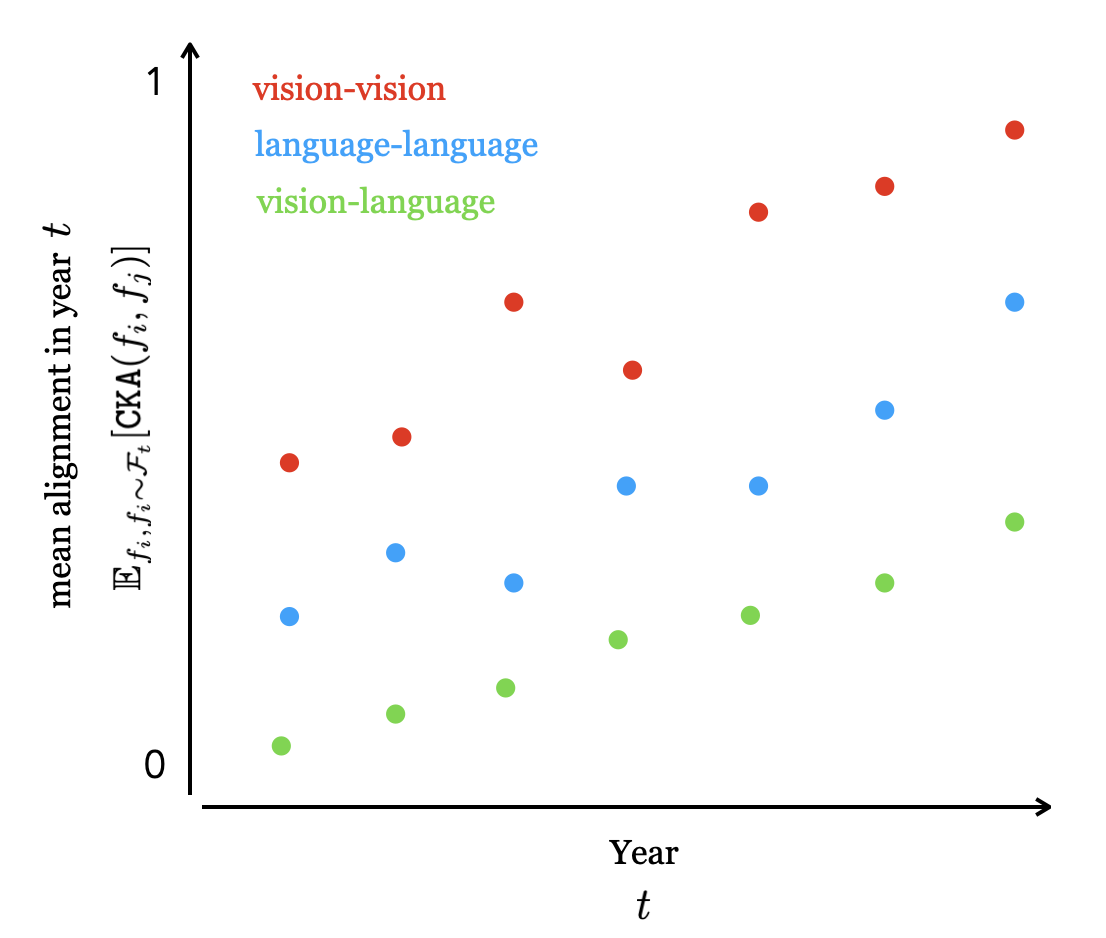
\includegraphics[width=1.0\linewidth]{figures/teaser.png}
%     \caption{Representations are converging over time. Why? And what are they converging to?}
%     \label{fig:convergence_over_time}
% \end{figure}

% TODO: \bc{Resolving the discrepancy between CKA and KNN, use KNN metric from metric evaluation paper}
% Resolve the analysis between rich vs small captions, fix the dataset change the richness of captions (recaption Wikipedia with simple captions or ImageNet with dense captions)
% Resolve what Plato actually meant about the shadows

\section{Introduction}

AI systems are rapidly evolving into highly multifunctional entities. For example, whereas in the past we had special-purpose solutions for different language processing tasks (\eg, sentiment analysis, parsing, dialogue), modern large language models (LLMs) are competent at all these tasks using a single set of weights~\cite{srivastava2022beyond}. Unified systems are also being built across data modalities: instead of using a different architecture for processing images versus text, recent models, such as GPT4-V~\cite{achiam2023gpt}, Gemini~\cite{team2023gemini}, and LLaVA~\cite{liu2023llava}, handle both modalities with a combined architecture. 
%become predominant, AI systems can take both images and text as input, and produce images or text as output. 
More and more systems are built off of general-purpose pretrained backbones, sometimes called foundation models~\cite{bommasani2021opportunities}, that support a large range of tasks, including robotics~\cite{driess2023palm,brohan2023rt}, bioinformatics~\cite{ma2024segment}, and healthcare~\citep{steinberg2021language}.
% self driving cars~\cite{XX}. 
%There's a discernible shift towards uniformity among various AI systems, with their architectures and capabilities becoming increasingly similar.
In short, AI systems are becoming increasingly homogeneous in both their architectures and their capabilities.


\begin{figure}[t]
    \centering
    \hypbox{The Platonic Representation Hypothesis}{%
    Neural networks, trained with different objectives on different data and modalities, are converging to a shared statistical model of reality in their representation spaces.}% shared representation of reality.}
%Neural networks, trained with different objectives on different data and modalities, will tend to converge to a common statistical model of reality.}
    \vspace{3pt}%common representation that captures a statistical model of the real world.}
    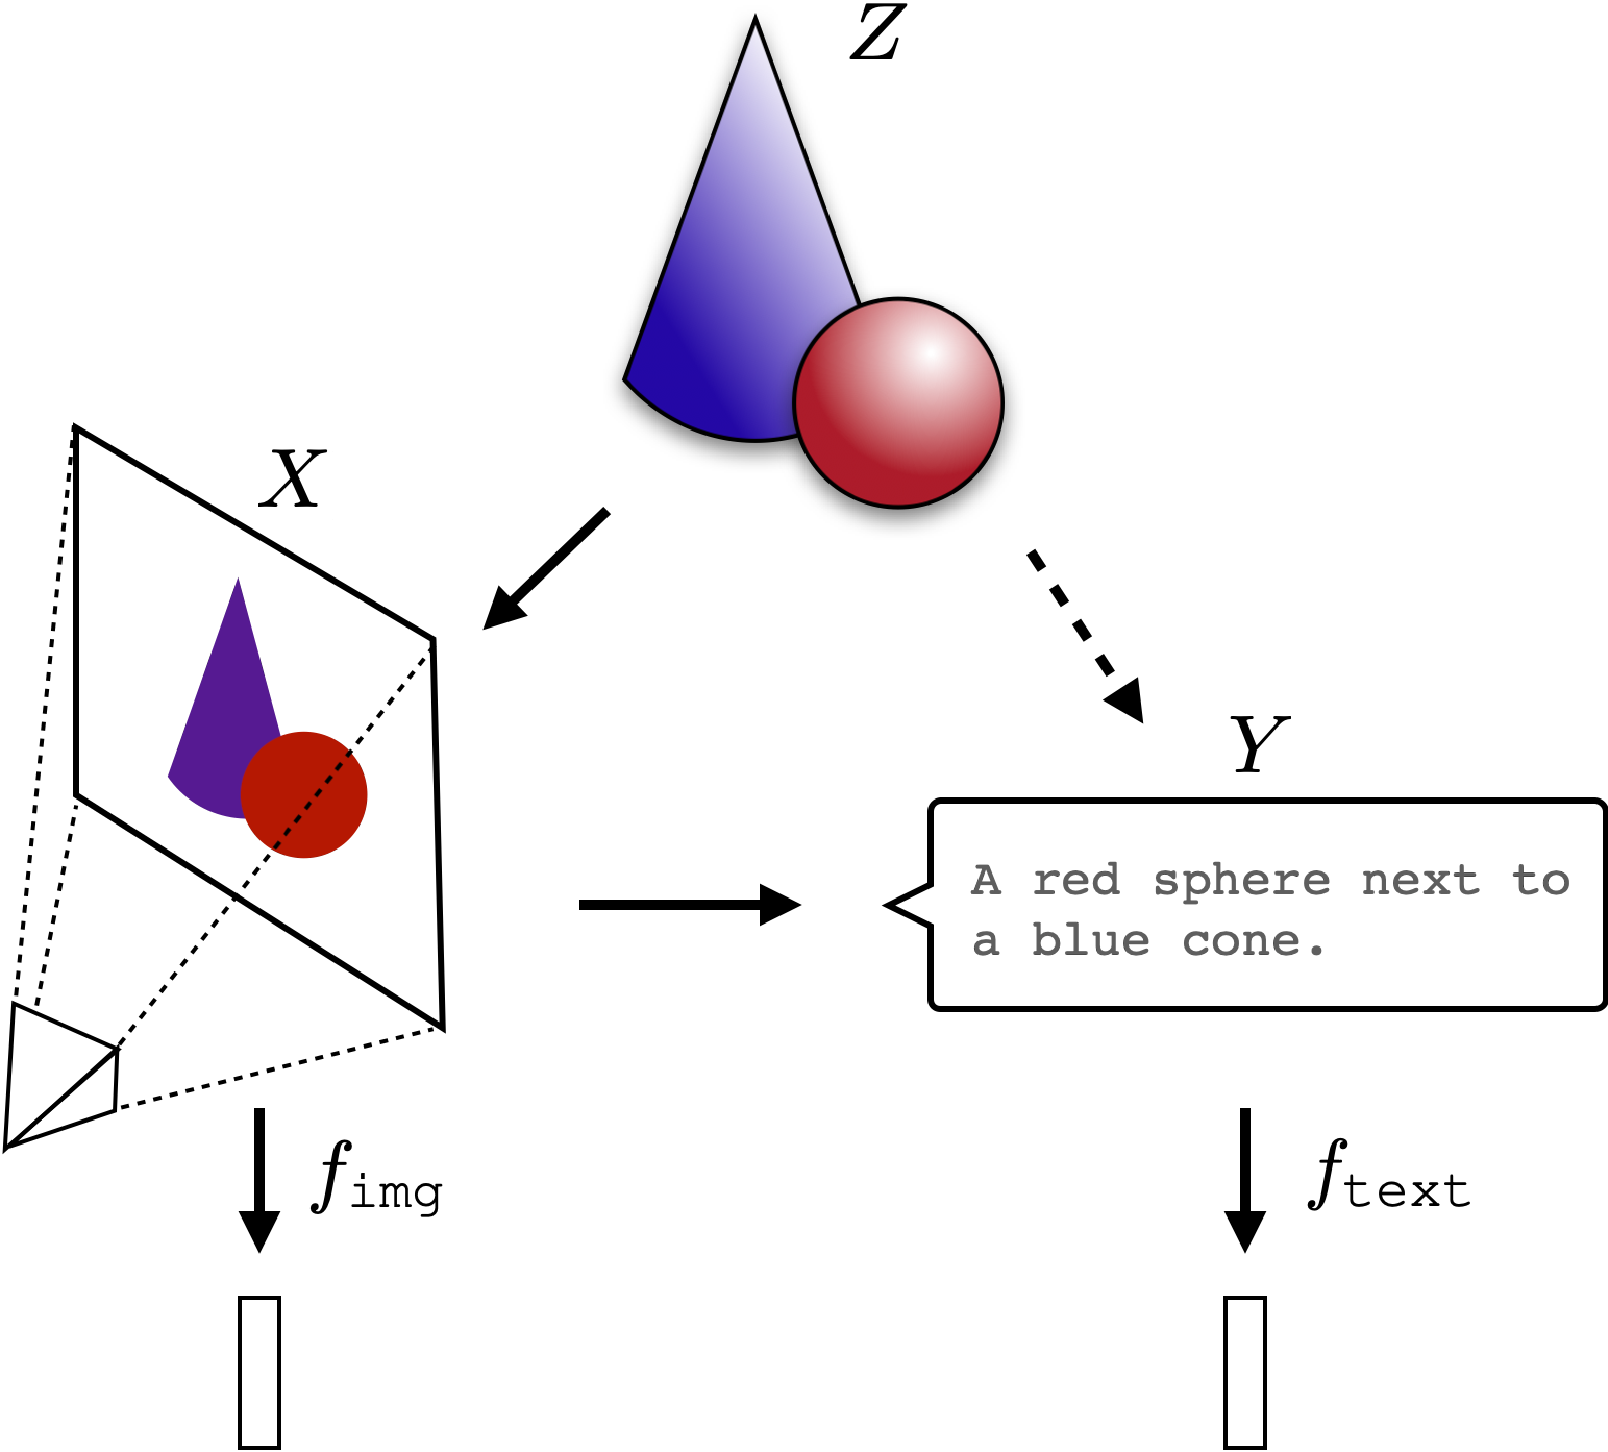
\includegraphics[width=0.85\linewidth]{figures/platonic_rep_less_space_v3.pdf}\vspace*{-5.5pt}
    \caption{\small \textbf{The Platonic Representation Hypothesis:} Images ($X$) and text ($Y$) are projections of a common underlying reality ($Z$). We conjecture that representation learning algorithms will converge on a shared representation of $Z$, and scaling model size, as well as data and task diversity, drives this convergence. %\fixme{rewrite with a short one now that we have the box here}
    %Our hypothesis is that there exists a real world out there (the shaded shapes), which we measure with various sensors, such as the camera shown to the left. Other \textit{views} of these measurements, such as the textual description shown, can be produced from the first set of measurements, or mediated by some other set of measurements (dotted arrow from A to C). Representation learning algorithms find vector embeddings that model the various measurements and views. The hypothesis is that the learned representations become reflections of the underlying physical world, and thereby converge upon the same metric space.
    }\label{fig:platonic_rep}
    % \vspace{-0.1in}
\end{figure}

This paper explores one aspect of this trend: representational convergence. We argue that there is a growing similarity in how datapoints are represented in different neural network models. This similarity spans across different model architectures, training objectives, and even data modalities.

What has led to this convergence? Will it continue? And ultimately, where does it end?

Our central hypothesis, stated above in \Cref{fig:platonic_rep}, is that there is indeed an endpoint to this convergence and a principle that drives it: different models are all trying to arrive at a \textit{representation of reality}, meaning a representation of the joint distribution over events in the world that generate the data we observe. \Cref{fig:platonic_rep} conveys this hypothesis: there exists a real world (labeled $Z$), which we measure with various sensors, such as the camera shown to the left ($X$). Other \textit{projections} of these measurements, such as the textual description shown, can be produced from the first set of measurements or mediated by some other set of measurements, \eg, touch or other camera views (dotted arrow from $X$ to $Y$)\footnote{Touch could convey the shapes in this example but not the colors. This is an important limitation to our hypothesis that we discuss at several points in the paper: different sensors and views might capture different information, which may limit their potential to converge to identical representations.
}. %\bc{Small nit: Touch won't be able to give adjectives like blue or red in the figure}
Representation learning algorithms find vector embeddings that statistically model the various measurements and projections. The resulting vector embeddings are all derived from the underlying reality in $Z$ and thereby become aligned. As models are trained on more data and for more tasks, they require representations that capture more and more information about $Z$, and hence alignment toward $Z$ increases toward a convergent point as a function of scale.

We call this converged hypothetical representation the ``platonic representation'' in reference to Plato's Allegory of the Cave~\cite{plato_cave}, and his idea of an ideal reality that underlies our sensations. The training data for our algorithms are shadows on the cave wall, yet, we hypothesize, models are recovering ever better representations of the actual world outside the cave. This idea is not unique to Plato; our hypothesis is also related to the notion of ``convergent realism''~\cite{newton1981rationality,putnam1982three,doppelt2007reconstructing,hardin1982defense} in the philosophy of science (\ie, that science is converging on truth), and to many arguments that have been put forth in the representation learning literature (\eg, \citet{tian2020contrastive,zimmermann2021contrastive,richens2024robust,cao2021explanatory}).

% \phil{Mention that people have also called this argument Anna Karenina or All roads lead to Rome.}

Also closely related to our hypothesis is the ``Anna Karenina scenario'' described by \citet{bansal2021revisiting}, referring to the possibility that all well-performing neural nets represent the world in the same way. We discuss the evidence they give for this possibility in \Cref{sec:reps_are_converging}\footnote{Borrowed from \citet{tolstoy1877anna}, similar analogies have been made in other domains, such as the ``Anna Karenina principle'' popularized by \citet{diamond1998guns} to explain animal domestication.}. The platonic representation hypothesis refers to the situation where we are in an Anna Karenina scenario \textit{and} the ``happy representation'' that is converged upon is one that reflects a statistical model of the underlying reality. We discuss the potential nature of this statistical model in more detail in \Cref{sec:what_rep}.%, where embeddings converge on a statistical model of the events that generate our sensory observations. In Section \ref{sec:what_rep}, we give a precise example such a statistical model that could be the convergent point.


% \begin{tcolorbox}[colback=white!95!black,colframe=white!30!black]
% \textbf{The Representational Convergence Hypothesis} 
% \\
% \\
% Different neural network architectures, trained on different datasets and data modalities, are converging to representations that are increasingly aligned in how they measure datapoint to datapoint distance.
% \end{tcolorbox}
% \begin{tcolorbox}[colback=white!95!black,colframe=white!30!black]
% \textbf{The platonic Representation Hypothesis} 
% \\
% \\
% Different neural network architectures, trained on different datasets and data modalities, will tend to converge to a common representation, as models, data, and compute are scaled. This representation reflects Plato's idea of ideal reality.
% \end{tcolorbox}

%The evidence for this convergence is found in a range of recent studies and meta-analyses. In earlier years, each AI subfield developed its unique methods and models. However, there has been a significant shift. This paper examines the factors contributing to this shift and explores its potential ramifications for the future of AI.
%\tz{add alignment of english vs ...}


%We posit that the field of AI is converging. This is evident when comparing the years 2014 and 2024. In 2014, the dominant architecture for computer vision was the Convolutional Neural Network (CNN), while for Natural Language Processing (NLP) it was the Recurrent Neural Network (RNN). Fast forward to 2024, and both fields predominantly use transformers. Similarly, in 2014, robots relied on handcrafted state representations, but now they increasingly use representations pretrained on vision or language tasks. This paper dives into the reasons and implications of such convergence. Specifically, we target the convergence of representations of signals across modalities and provide our perspectives on several key questions: 

%What has led to this convergence? Will it continue? And ultimately, where does it end? Our central thesis is that representations are converging towards a unified metric space. This convergence can be observed over time, model scale, and performance: bigger, better, and more recent models are more alike. We argue that 1) representations are indeed converging, 2) this convergence is unlocking numerous new opportunities for leveraging these unified models, and 3) these representations are progressing towards a probabilistic model of the underlying physical state of the world.

% As artificially intelligent systems become more capable, they are increasingly subjected to selective pressure of needing to achieve goals and perform tasks in various real-world environments. Systems that are too narrowly specialized will fail or be limited. Just as convergent evolution leads biological species to develop similar adaptive traits when facing similar environmental pressures, the pressure for general intelligence is causing different AI systems to develop similar underlying competencies and mechanisms.

% The community's objective of achieving human-level intelligence, defined by its generality across environments, requires the development of learning and adaptation abilities to achieve goals across many contexts flexibly. This pressure towards general competency is nudging different AI architectures in similar directions, leading to convergence.




%By analyzing the trajectory of AI development from 2014 to 2024, this paper aims to shed light on the ongoing convergence in AI representations. We discuss how this convergence has emerged, its current state, and its possible future, focusing on the convergence of representations across different modalities and its implications for the field of AI as a whole.

%\section{Defining Intelligence}

% If we define intelligence as the ability to achieve goals across environments \cite{legg2008machine}, then the evolutionary pressure on AI systems to develop versatile, general capabilities can explain why continued advances in AI may lead to convergence, as this pressure shapes the emergence of the competencies and mechanisms needed for broad, human-like intelligence.

%If we adopt the definition of intelligence as the ability to achieve goals in various environments~\cite{legg2008machine}, then the evolutionary pressures on AI systems to develop versatile and general capabilities provide a plausible explanation for the ongoing convergence in AI advancements. These pressures are likely to guide the development of competencies and mechanisms necessary for achieving broad, human-like intelligence.

\vspace{-3pt}
\section{Representations are converging}\label{sec:reps_are_converging}

\paragraph{Preliminaries}
We restrict our attention to representations that are \textit{vector embeddings}. We characterize such a representation by the similarity structure it induces, referred to as its kernel. Kernels are commonly used to assess representations~\cite{kornblith2019similarity, klabunde2023similarity}; this can be justified by the fact that they capture the relative structures among data samples, which are also the learning signal for many machine learning algorithms ~\cite{aronszajn1950theory,smola1998learning}. Following prior literature, we define \textit{representational alignment} as a measure of the similarity of the similarity structures induced by two representations, \ie, a similarity metric over kernels.
% distance\footnote{We use the terms ``distance'' and ``metric'' loosely, as an index that is high for very different items and low for similar items; we do not mean a distance metric as rigorously defined in mathematics.} between kernels.
We give the mathematical definition of these concepts below:
\begin{itemize}[topsep=-1.5pt,itemsep=-1.5pt,leftmargin=10pt]
    \item A \textbf{representation} is a function $f\colon \mathcal{X} \rightarrow \mathbb{R}^n$ that assigns a feature vector to each input in some data domain $\mathcal{X}$. %vector of features generated by a model for a given input. %These vectors capture the essential information from the input data, as deemed relevant by the model for performing a specific task.
    \item A \textbf{kernel}, $K\colon \mathcal{X} \times \mathcal{X} \rightarrow \mathbb{R}$, characterizes how a representation measures distance/similarity between datapoints. $K(x_i,x_j) = \langle f(x_i), f(x_j) \rangle$, where $\langle {{}\cdot{}},{{}\cdot{}}\rangle$ denotes inner product, $x_i, x_j \in \mathcal{X}$ and $K \in \mathcal{K}$.
    \item A \textbf{kernel-alignment metric}, $m\colon \mathcal{K} \times \mathcal{K} \rightarrow \mathbb{R}$, measures the similarity between two kernels, \ie, how similar is the distance measure induced by one representation to the distance measure induced by another. Examples include Centered Kernel Distance (CKA)~\cite{kornblith2019similarity}, SVCCA~\cite{raghu2017svcca}, and nearest-neighbor metrics~\cite{klabunde2023similarity}.
    %$K: \mathcal{X} \times \mathcal{X} \rightarrow \mathbb{R}$ Measures used to quantify the similarity of features generated by two models. Metrics assess how closely aligned the representations are. $K_{mnn}$ refers to the mutual nearest-neighbor metric describe in detail in the Section \ref{sec:alignment_methods}.
    %\item \textbf{Mutual nearest-neighbor metric:} A nearest-neighbor similarity metric, $m: \mathcal{X}_1 \times \mathcal{X}_2 \rightarrow \mathbb{R}$, that measures the intersection of the $k$-nearest neighbors of two representations for two arbitrary domains $\mathcal{X}_1,\mathcal{X}_2 $. The intersection is normalized by $k$ and is related to the neighborhood similarity metric of \citet{klabunde2023similarity}.
\end{itemize}

% \tz{oron2017best has a very similar metric. maybe worth add a citation too.}
In our experiments, we use a \emph{mutual nearest-neighbor metric} that measures the mean intersection of the $k$-nearest neighbor sets induced by two kernels, $K_1$ and $K_2$, normalized by $k$.
% , which we refer to as $m_{\texttt{NN}}$. 
This metric is a variant of those proposed in~\citet{park2024quantifying}, \citet{klabunde2023similarity} and \citet{oron2017best}.
% ; $m_{\texttt{NN}}(K_1, K_2)$ measures the mean intersection of the $k$-nearest neighbor sets induced by two kernels, $K_1$ and $K_2$, normalized by $k$. %The intersection %is normalized by $k$ and is 
% This metric is related to the neighborhood similarity metric of \citet{klabunde2023similarity}. 
See~\app{sec:align-metric} for the exact definition and~\app{app:other-metrics} for comparisons with alternative alignment metrics.
% \todo{put other metric results in appendix}
% \app{sec:other-metrics} replicates the our experiments with other metrics, showing similar trends. \fixme{add} 

%Moving some old text here: The use of kernels in characterizing representations, where similarity is determined by the similarity of kernels, has a long history. Metrics like representation dissimilarity matrices (RDMs) and centered kernel alignment (CKA) have been used to measure similarities of models of varying architectures~\citep{XX}, suggesting that they converge to similar kernels~\citep{XX}. 

%This work relies on mutual nearest-neighbor metric, choice based on the limitations of existing metrics such as CKA and SVCCA. These metrics have a stricter definition alignment, which may not fit our current needs. 
%For instance, understanding the precise relationship between unrelated items, such as an apple and Bill Gates, or the exact distances among a dog, a cat, and a bowl of cereal, may not be critical. It's more important to recognize that a dog and cat are likely to co-occur than either is to a cereal bowl. For similar reasons, existing works relied on alternative metrics such as model-stitching as it ``reveals aspects of representations that measures such as centered kernel alignment (CKA) cannot''~\cite{bansal2021revisiting}.


% \begin{itemize}
%     \item \textbf{Mutual nearest-neighbor metric:} A nearest-neighbor similarity metric, $m: \mathcal{X}_1 \times \mathcal{X}_2 \rightarrow \mathbb{R}$, that measures the intersection of the $k$-nearest neighbors of two representations for two arbitrary domains $\mathcal{X}_1,\mathcal{X}_2 $. The intersection is normalized by $k$ and is related to~\citet{klabunde2023similarity} neigborhood similarity metric.
%     % image-text pair $(x_{\mathsf{image}}, x_{\mathsf{text}})$, we pass image $x_{\mathsf{image}}$ through vision model and $x_{\mathsf{text}}$ through the language model and measure its intersection of neighbors.
% \end{itemize}

% \jh{putting this here for you brian}
% First, to measure alignment, we use the nearest-neighbor metric on paired caption data, a choice based on the limitations of existing metrics like CKA~\cite{kornblith2019similarity} and SVCCA~\cite{raghu2017svcca}. These metrics have a stricter definition alignment, which may not fit our current needs. 
% For instance, understanding the precise relationship between unrelated items, such as an apple and Bill Gates, or the exact distances among a dog, a cat, and a bowl of cereal, may not be critical. It's more important to recognize that a dog and cat are likely to co-occur than either is to a cereal bowl.

% For similar reasons, existing works relied on alternative metrics such as model-stitching as it
% ``reveals aspects of representations that measures such as centered kernel alignment (CKA) cannot''~\cite{bansal2021revisiting}. However, for billion parameter models, this becomes quickly infeasible to scale, and we have opted for a simpler metric of mutual nearest-neighbors~\cite{klabunde2023similarity}. Given an image-text pair $(x_{\mathsf{image}}, x_{\mathsf{text}})$, we pass image $x_{\mathsf{image}}$ through vision model and $x_{\mathsf{text}}$ through the language model and measure its intersection of neighbors. A greater overlap between the neighbor sets implies better alignment between the models. Although mutual nearest-neighbor has its own quirks and issues, we use it as proxy for examining alignment between vision and language models. Further investigation is needed to identify a more accurate metric for alignment measurement. See~\app{sec:alignment_methods} for further details and discussion.


Next, we explore several ways in which representations are converging. First, we argue that different neural networks are converging to aligned representations. Then, we show that this continues to hold across modalities, where image embeddings in vision models align with text embeddings in language models.
% Finally, we discuss the related literature on alignment between biological brains and neural nets, which has also found a generally increasing trend.


%\paragraph{Large models, representation reuse, and fine-tuning}
%If the hypothesis that representations are converging is true, it must also follow that the more accurate the representation is to the underlying physical laws, the better the model should be for fine-tuning across various tasks.
%In fact, this has become more evident than ever with a growing emphasis on adapting large pre-trained models. Without tuning such models, their representations already demonstrate high performance on many tasks these models are not trained on, such as information retrieval \citep{babenko2016efficient}, making analogies \citep{mikolov2013efficient} or even as training signal to learn on a new modality \citep{zhai2022lit}. 

%While the idea of representational generalization is not new ~\cite{rumelhart1985learning}, the benefits appear to be amplified when fine-tuning from large models and models with better representations. 
%Observations include the need for fewer samples to converge~\cite{zhou2023lima,kirstain2021few}, modality agnostic generalization~\cite{lu2021pretrained}, reduced forgetting of prior tasks~\cite{ramasesh2022effect,mehta2021empirical,mirzadeh2022wide}, the optimization requirement of low-rank estimates~\cite{hu2021lora}, and the ability to optimize finetuned models in tangent space~\cite{ortiz2023task}. These empirical findings suggest that large models may have converged to a representation that is somewhat locally connected to parameters that can generalize to other tasks~\cite{neyshabur2020being, ainsworth2022git, lubana2022mechanistic, juneja2022linear}. This notion has been termed the "Superficial Alignment Hypothesis," which posits that a model's knowledge and capabilities are primarily acquired during pretraining, and alignment occurs through movement within that basin~\cite{zhou2023lima}.

%The motivation of this paper is that it \textit{feels like} AI representations are converging. We ran the following experiment to test if this feeling is valid.

% We measure how similar one model is to another using \texttt{CKA} and nearest-neighbors. This metric assigns a high score to two models if they represent inputs in a similar way. In particular, $\texttt{CKA}(f_A,f_B)$ measures the similarity between the way model $f_A$ measures distance between inputs and the way model $f_B$ measures distance between the same inputs\footnote{Or matching inputs. If $f_A$ is an image encoder and $f_B$ is a text encoder, then \texttt{CKA} checks if $f_A$ measures distance between images in the same way as $f_B$ measures distance between the captions for those same images.}. Models $f_A$ and $f_B$ are both functions $\mathcal{X} \rightarrow \mathbb{R}^N$ that induce a distance metric $\norm{f_A(x_i) - f_A(x_j)}$. \texttt{CKA} is a standard method in the field of representational alignment \cite{XX}; we defer further discussion of it to the appendix.

% Instead we use a nearest-neighbor metric.

% \begin{figure*}[t!]
%     \centering
%     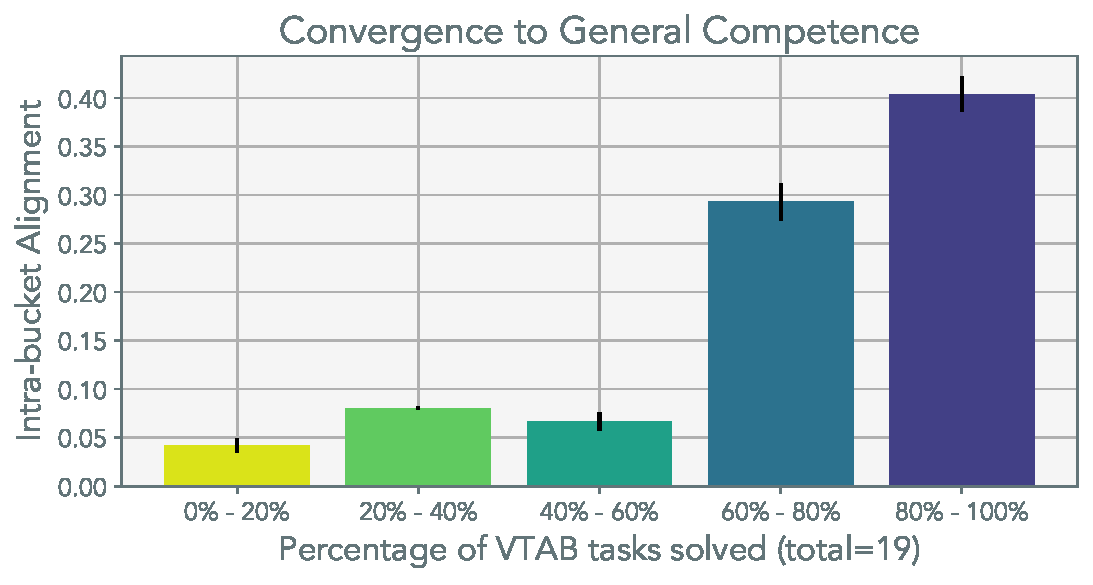
\includegraphics[width=0.6077\linewidth]{figures/vision_align_bucket_bar_plot_separate_data.pdf}\hfill%
%     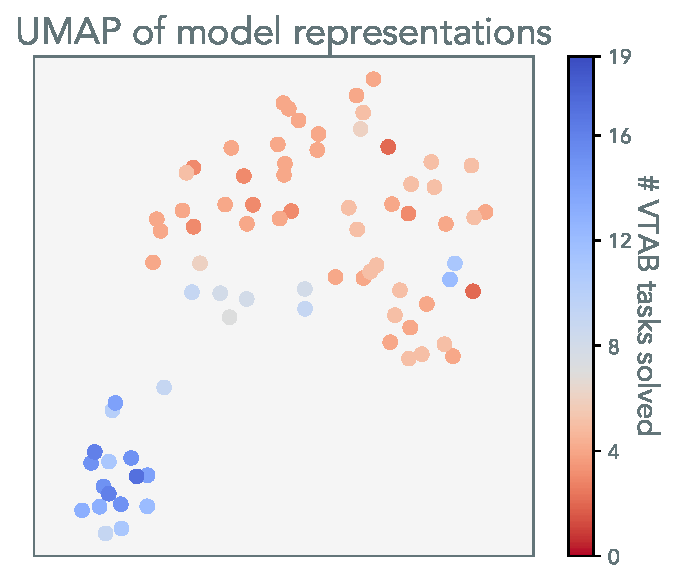
\includegraphics[width=0.374\linewidth]{figures/vision_align_scatter_plot_separate_data.pdf}\\[-0.175in]
%     \caption{\small \textbf{VISION models converge as COMPETENCE increases:} We measure the alignment among $78$ vision models as the representations become more competent at solving diverse downstream tasks on the Visual Task Adaptation Benchmark (VTAB; \citet{zhai2019vtab}). Alignment is measured according to the mutual nearest-neighbor measure on VTAB data. \textbf{LEFT:} Models that solve more VTAB tasks tend to be more aligned. Error bars show standard error. \textbf{RIGHT:} We use UMAP to embed models into a 2D space for visualization, based on $\mathsf{distance} \triangleq -\log (\mathsf{alignment})$. More competent and general models (blue) have more similar representations. 
%     % \fixme{make it more concise; update with jacob's plots}
%     }
%     \label{fig:vm_align}
% \end{figure*}

% \begin{figure}[t!]
%     \centering
%     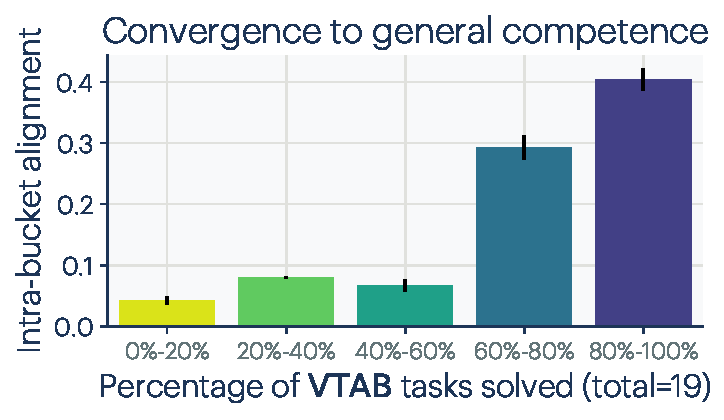
\includegraphics[width=0.95\linewidth]{figures/vision_align_bucket_bar_plot_separate_data_single_col_____mnn_1000.pdf}\\[0.02in]%
%     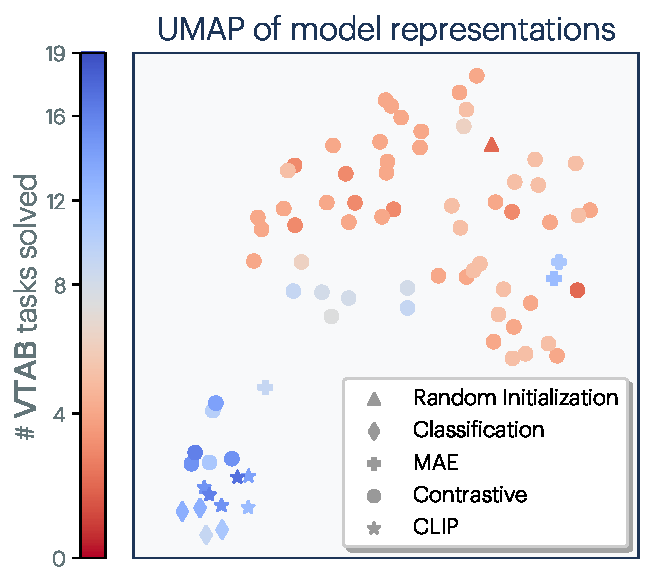
\includegraphics[width=0.95\linewidth]{figures/vision_align_scatter_plot_separate_data_left_cbar_labelled_____mnn_1000.pdf}\\[-0.15in]
%     \caption{\small \textbf{VISION models converge as COMPETENCE increases:}  We measure alignment among $78$ models using mutual nearest-neighbor on Places-365 \citep{zhou2017places}, and evaluate their representations on diverse downstream tasks from the Visual Task Adaptation Benchmark (VTAB; \citet{zhai2019vtab}). \textbf{TOP:} Models that solve more VTAB tasks tend to be more aligned. Error bars show standard error. \textbf{BOTTOM:} We use UMAP to embed \emph{models} into a 2D space for visualization, based on $\mathsf{distance} \triangleq -\log (\mathsf{alignment})$. More competent and general models (blue) have more similar representations. }%
%     \label{fig:vm_align}
% \end{figure}


\begin{figure*}[ht!]
    \vspace{-2pt}
    \begin{minipage}[t]{0.65\textwidth}
        \hspace{-0.1in}
        % \hspace{-0.1in}
        % \raisebox{-\height}{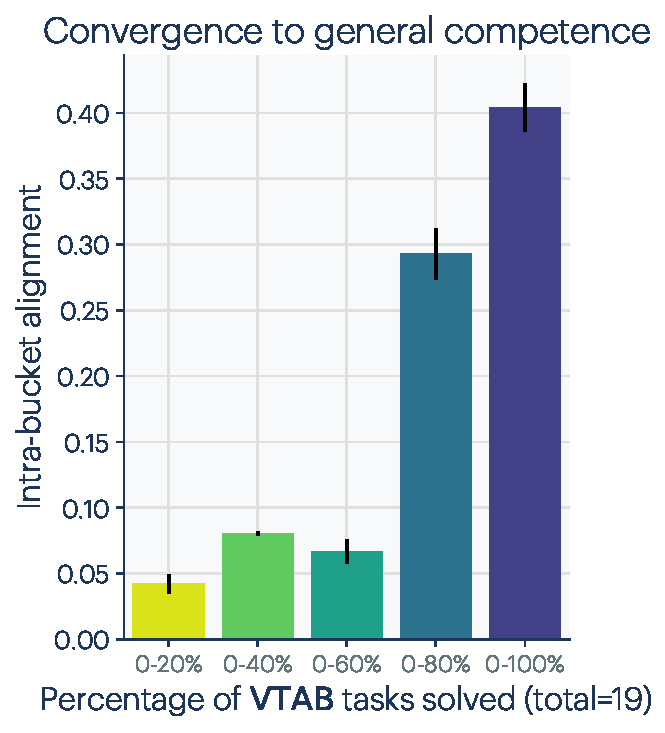
\includegraphics[width=0.4675\linewidth, trim=0 0 0 0]{figures/vision_align_bucket_bar_plot_separate_data_single_col_vertical_____mnn_1000.pdf}}
        \raisebox{-\height}{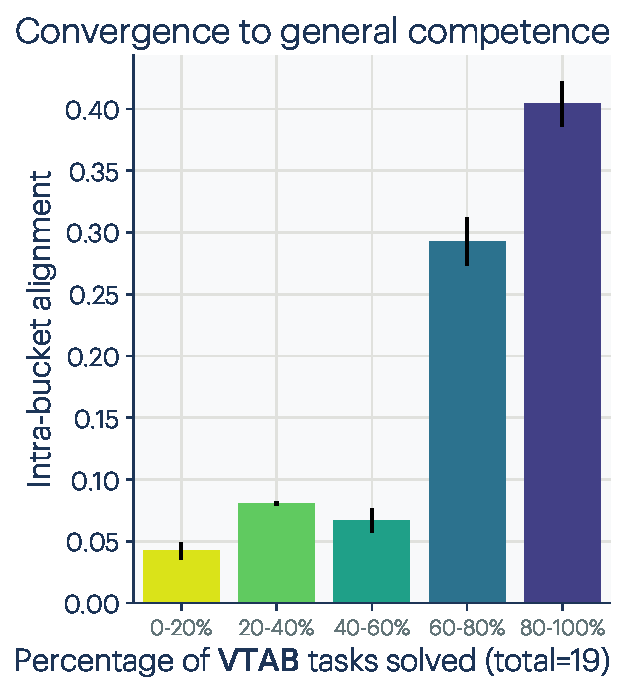
\includegraphics[width=0.47\linewidth, trim=0 0 0 0]{figures/vision_align_bucket_bar_plot_separate_data_single_col_vertical_v3_____mnn_1000.pdf}}
        % \hspace{-0.124in}
        % \hspace{-0.2in}
        \raisebox{-\height}{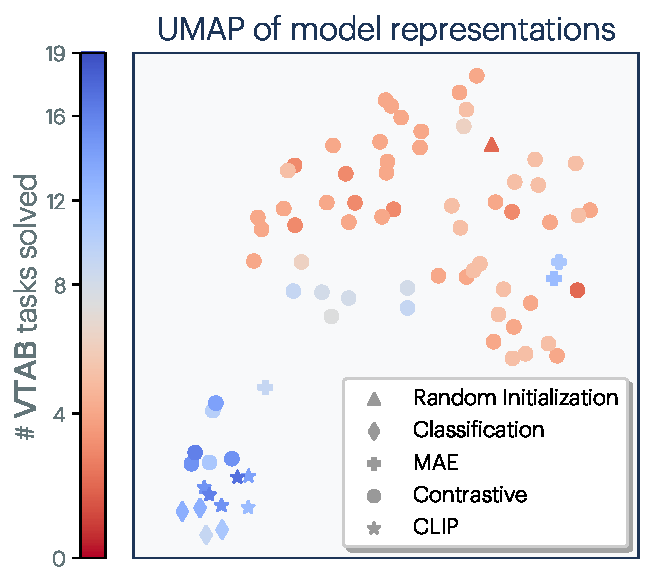
\includegraphics[width=0.504\linewidth, trim=5 0 11 0]{figures/vision_align_scatter_plot_separate_data_left_cbar_labelled_____mnn_1000.pdf}}
        \hfill
    \end{minipage}%
    \hfill
    \begin{minipage}[t]{0.35\textwidth}
        \vspace{-0.075in}
        \caption{%
            \small \textbf{VISION models converge as COMPETENCE increases:} We measure alignment among $78$ models using mutual nearest-neighbors on Places-365 \cite{zhou2017places}, and evaluate their performance on downstream tasks from the Visual Task Adaptation Benchmark (VTAB; \citet{zhai2019vtab}). \textbf{LEFT:} Models that solve more VTAB tasks tend to be more aligned with each other. Error bars show standard error. \textbf{RIGHT:} We use UMAP to embed \emph{models} into a 2D space, based on $\mathsf{distance} \triangleq -\log (\mathsf{alignment})$. More competent and general models (blue) have more similar representations.}
        \label{fig:vm_align}
    \end{minipage}
    \vspace{-16pt}
\end{figure*}
% \begin{figure*}[t!]
%     \begin{minipage}[c]{0.305\textwidth}
%         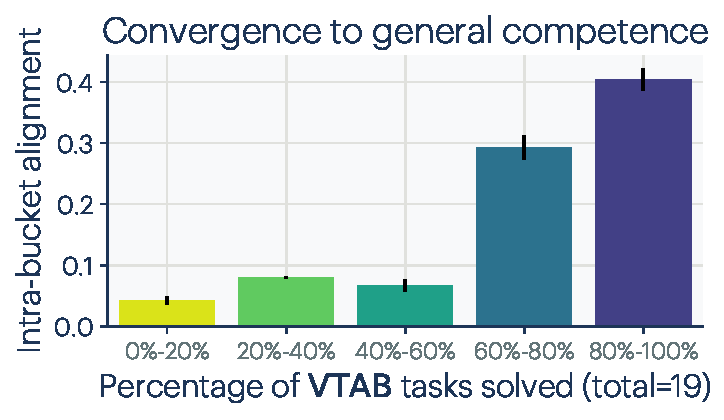
\includegraphics[width=\linewidth]{figures/vision_align_bucket_bar_plot_separate_data_single_col_____mnn_1000.pdf}
%     \end{minipage}
%     \begin{minipage}[c]{0.36\textwidth}
%         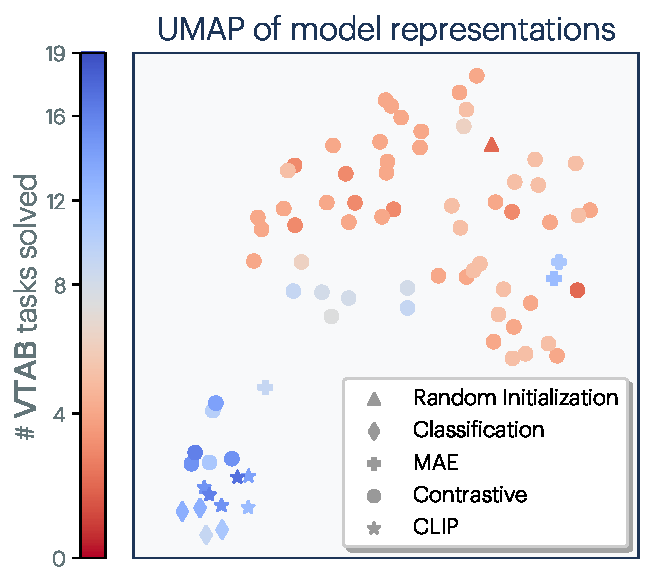
\includegraphics[width=\linewidth]{figures/vision_align_scatter_plot_separate_data_left_cbar_labelled_____mnn_1000.pdf}
%     \end{minipage}%
%     \hfill
%     \begin{minipage}[c]{0.325\textwidth}%
%         \vspace{-6pt}
%         \caption{\small \textbf{VISION models converge as COMPETENCE increases:} We measure alignment among $78$ models using mutual nearest-neighbor on Places-365 \citep{zhou2017places}, and evaluate their representations over diverse tasks from the Visual Task Adaptation Benchmark (VTAB; \citet{zhai2019vtab}). \textbf{LEFT:} Models that solve more tasks are more aligned. Error bars show standard error. \textbf{RIGHT:} We use UMAP to embed \emph{models}  for visualization, based on $\mathsf{distance} \triangleq -\log (\mathsf{alignment})$. Competent and general models (blue) have similar representations. 
%         }\label{fig:vm_align}
%     \end{minipage}
% \end{figure*}

\subsection{Different models, with different architectures and objectives, can have aligned representations}

% \bc{Though "All roads lead to Rome" is a common phrase, maybe we should cite https://arxiv.org/pdf/2106.07682.pdf which makes the same case with the same phrase}
%\paragraph{Representational Convergence: All roads lead to Rome.}

One indication of representational convergence is the rising number of systems built on top of pre-trained foundation models. These models are becoming standard backbones across a growing spectrum of tasks. Their versatility across numerous applications implies a level of universality in the way they represent data. %This suggests the existence of a singular underlying representation that supports a myriad of tasks across different domains.

% A clear indication that representations are converging is the abundance of papers that use a pretrained model as their backbone, a.k.a. a foundation model. This approach is being increasingly adopted for a wider variety of tasks. The ability of these models to adapt to a wide range of applications suggests a certain universality in the backbone's underlying data representation; a single representation that supports a myriad of tasks across different domains.

%All models that are adapted from a given foundation model must be within a certain distance of the same representation, determined by the type and degree of adaptation. Indeed, it is common to freeze the foundation model and directly use its data representation for new AI systems, in which case all these systems can be said to rely on the same underlying representation.

% While this trend implies some degree of convergence, it does not imply that \textit{different} foundation models will arrive at the same representation. Yet that is what has been observed by several recent papers. One avenue has been to analyze representational similarity via model stitching. This approach, initially proposed by \citet{lenc2015understanding}, considers two models, $f$ and $g$, which are assumed to each consist of a composition of layers, $f = f_1 \circ \ldots \circ f_n$, $g = g_1 \circ \ldots \circ g_m$. An intermediate representation from $f$ and is fed to $g$, mediated by an affine ``stitching layer'' $h$, resulting in $F = f_1 \circ \ldots \circ f_k \circ h \circ g_{k+1} \circ \ldots \circ g_m$, where $h$ is optimized to align the models. If the model net, $F$, maintains good performance, then we can say that $f$ and $g$ have compatible representations on layer $k$, up to affine transformation $h$. 

%The trend above suggests a weaker notion of convergence. It does not necessarily mean different foundation models are converging into a single platonic ideal. 
While this trend implies convergence toward a relatively small set of foundation models, it does not imply that \textit{different} foundation models will arrive at the same representation. Yet that is what has been observed by several recent papers. 
%However, recent studies have observed that even the representations themselves may indeed be converging. 

\citet{lenc2015understanding} conducted one such study, in which they measured representational similarity through a technique called \textit{model stitching}. Given two models, $f$ and $g$, each composed of multiple layers ($ f = f_1 \circ \cdots \circ f_n $, $ g = g_1 \circ \cdots \circ g_m $), an intermediate representation from $f$ is integrated into $g$ via a learned affine stitching layer $ h $, resulting in a new stitched model $F = f_1 \circ \cdots \circ f_k \circ h \circ g_{k+1} \circ \cdots \circ g_m $. %The layer $h$ is optimized to align the models. 
If $F$ has good performance, it indicates that $f$ and $g$ have compatible representations at layer $k$, up to the  transform $h$.
% , up to
% affine transformation $h$.

% Moreover, \citet{lenc2015understanding} found that 1) a vision model trained on ImageNet~\cite{russakovsky2015imagenet} can be aligned with one trained on the Places dataset~\citep{zhou2017places} and maintain high performance, and 2) that early layers in these convolutional networks are more interchangeable. The first point demonstrates a degree of data independence: two rather different image distributions induce similar representations. The second point agrees with the large body of work that has shown that oriented Gabor-like filters show up in numerous artificial and biological vision systems -- the first layer of representation in all kinds of neural nets seems to arrive at this same representation~\citep{olshausen1996emergence, krizhevsky2017imagenet}.


In their study,~\citet{lenc2015understanding} made two notable findings: (1) A vision model trained on ImageNet~\cite{russakovsky2015imagenet} can be aligned with a model trained on Places-365~\citep{zhou2017places} while maintaining good performance; (2) The early layers of these convolutional networks are more interchangeable than later layers. The first finding illustrates a level of data independence where distinct image datasets lead to similar representations. The second finding agrees with extensive research that oriented Gabor-like filters are common in both artificial and biological vision systems. This suggests a convergence to a similar initial layer of representation across various neural network architectures~\citep{olshausen1996emergence, krizhevsky2017imagenet}.
\citet{bansal2021revisiting} expanded on the idea of model stitching, showing that models trained using self-supervised objectives align closely with their supervised counterparts.


% This idea was revisited by~\citet{bansal2021revisiting}, where they further explored model stitching, notably finding that representations trained with a self-supervised objective are well aligned with representations trained with supervised objectives.

% Later,~\citet{moschella2022relative} showed that models can even be stitched in a \textit{zero shot} fashion, without a learnable stitching layer. They observed that while two models might use somewhat different representations, the representations are often remarkably similar in terms of \textit{how they measure distance}. Therefore, the feature kernel can be used as a zero-shot interface between models: from an encoder $f$ that maps data to embeddings, a feature kernel $K$ can be extracted. This can be directly glued to a decoder that maps kernels to predictions. An interesting finding was that the encoder can be trained on one language (\eg, English) and the decoder can be \textit{independently} trained on another language (\eg, French). The English encoder yields an English-trained kernel while the decoder starts from a French-trained kernel, yet they work when glued together because the kernel is, roughly, invariant to language type! This finding is consistent with other work that has shown that different human languages share very similar similarity structure~\cite{XX}.

% Building on this concept,~
\citet{moschella2022relative} further demonstrated the feasibility of ``zero-shot'' model stitching without learning a stitching layer.
% , eliminating the need for a learnable stitching layer. 
Despite the fact that different text models were trained on different modalities, they found that the models often
embed data in remarkably similar ways. In particular, they considered the kernel $K$ defined by learned representations and showed that $K$ serves as a bridge between models, allowing an encoder trained in one language, like English, to work effectively with a decoder in another, like French. %This aligns with broader research indicating that different human languages exhibit a very similar structure of similarities.~\cite{XX}.
%they considered the kernel $K$ defined by learned representations and showed that

\citet{dravid2023rosetta} extended this idea to individual neurons, and found ``Rosetta Neurons'' that are activated by the same pattern across a range of vision models. Such neurons form a common dictionary independently discovered by all models.

%layer $that there exttaist ``k$ represroseentations, $f_k$ and $g_k$, in two models $f$ and $g$ can often be aligned simply via a linear transformation, as was shown in the previous stitching papers. When this is the case, the feature kernels on the $k$-th layer must be similar, because kernels are invariant to linear 

%The concept of model stitching, where different models are combined, was initially explored in the work of~\cite{lenc2015understanding}. They demonstrated the effectiveness of stitching together multiple models to improve performance. Similarly, stitching together models trained on different data and/or objectives (but share the same representation) can achieve surprising transfer capabilities, such as semantic classification on a language that the classifier is never trained on \citep{moschella2022relative}.
% A related idea is the use of averaging in convex problems, as highlighted by ~\cite{scaman2019optimal}in their study on optimal averaging. 
%\cite{bansal2021revisiting} demonstrated stitching the top and bottom half of two independently pre-trained models could successfully learn the same representation -- an ``Anna Karenina" scenario where all good models converge to a similar solution.

% The use of kernels as a way to characterize representations has a long history, in which two representations are considered to be similar if their kernels are similar. Representational similarity metrics based on kernels include RDMs and CKA. Studies using these metrics have come to similar conclusions to those based on stitching, including that differently trained nets arrive at similar kernels~\citep{XX} and different architectures may also arrive at similar kernels~\cite{XX}.

% \citet{kornblith2019similarity}~identified a further phenomenon, where not only are models often well aligned, the degree of alignment increases with scale. They trained neural networks of different widths multiple times on the CIFAR10 classication dataset. Then they measured the mean CKA between pairs of models of the same width (from different training runs). This value increased the wider the models got, indicated that wider models are more aligned with each other than narrower models are with each other. As we expect models to continually be scaled up over time, this trend suggests that models will become more aligned.


% \begin{figure*}[t!]
%     \centering
%     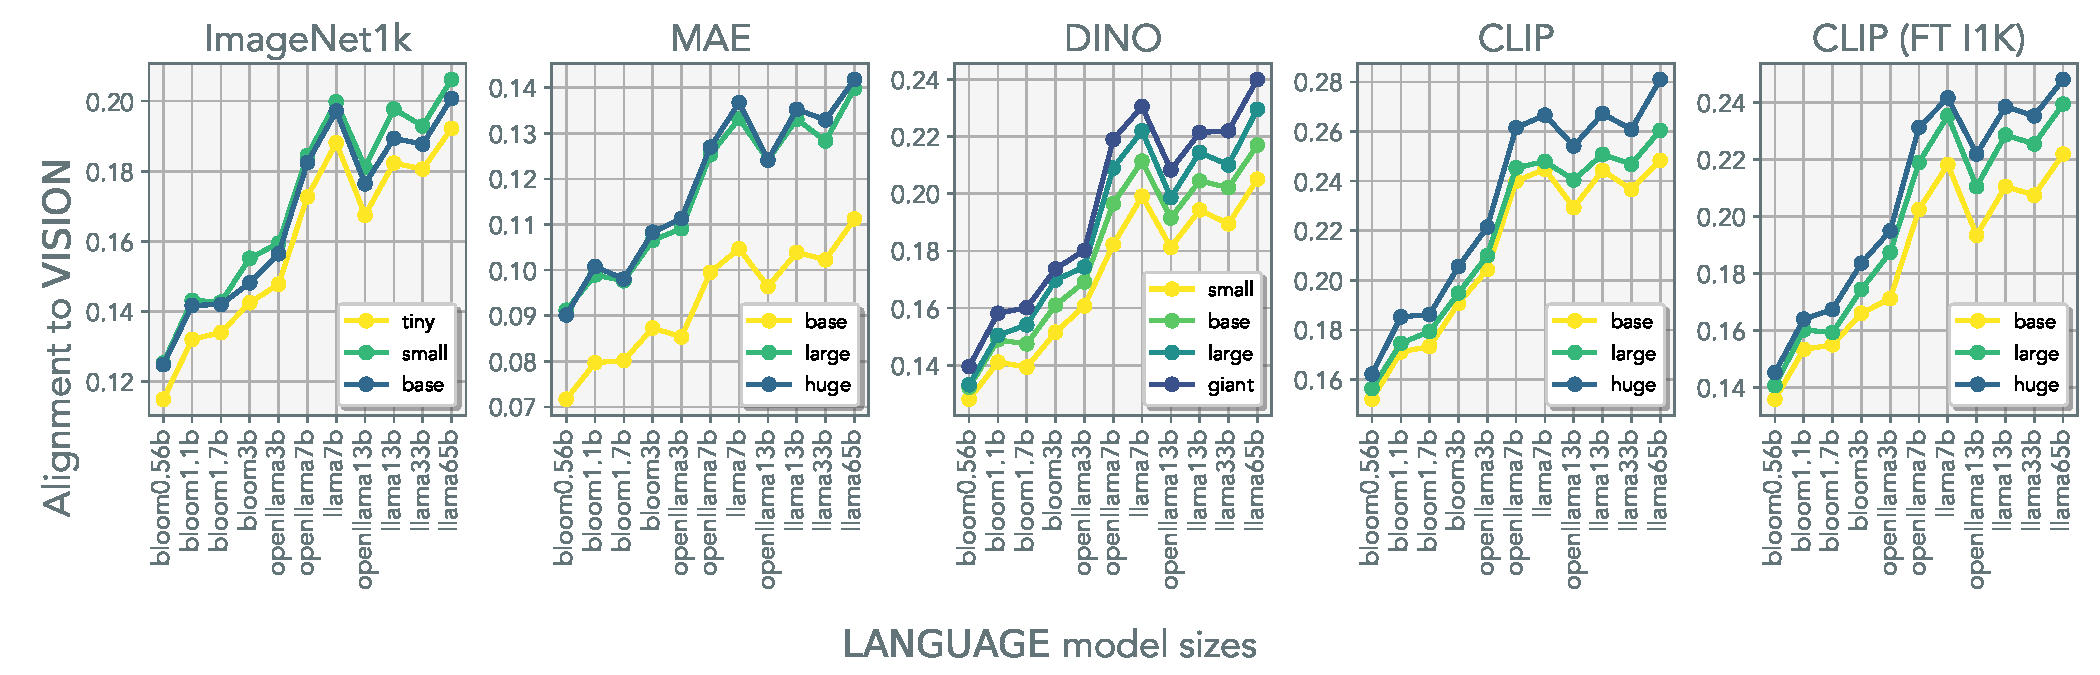
\includegraphics[width=1.\linewidth]{figures/llm_alignment_per_task.pdf}\\[-0.1in]
%     \caption{\small \textbf{LANGUAGE models align with VISION:} We measure the alignment of language models to vision models for each vision task. Language models are ordered by size. Alignment is a measure of the mutual nearest-neighbor on Wikipedia caption dataset (WIT). For most tasks we see a consistent trend, larger language models are more aligned with vision models.}
%     \label{fig:llm2lvm_align}
% \end{figure*}
% \begin{figure*}[t!]
%     \centering
%     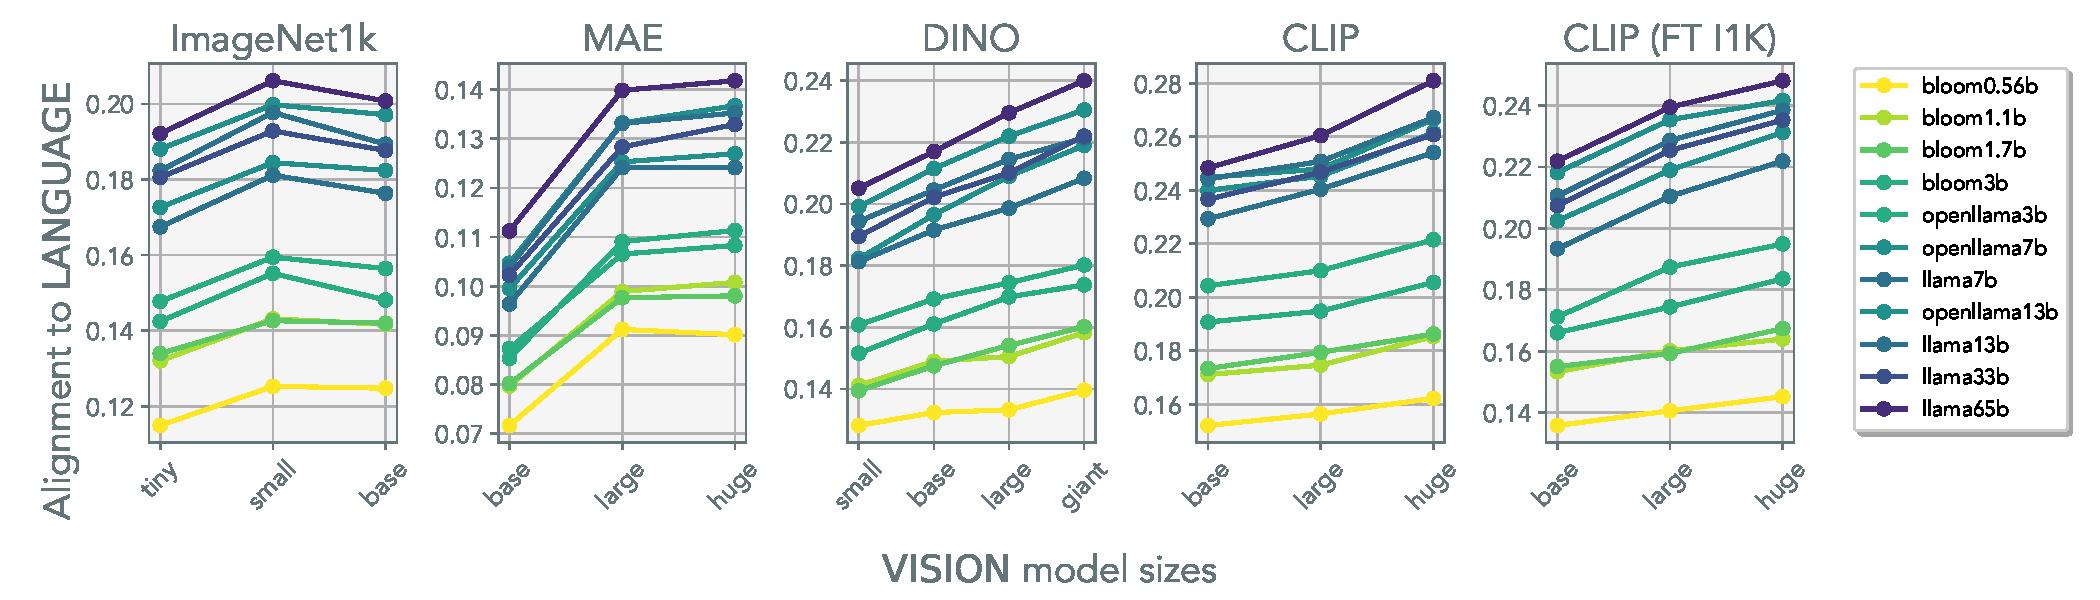
\includegraphics[width=1.0\linewidth]{figures/lvm_alignment_per_task.pdf}\\[-0.1in]
%     \caption{\small \textbf{VISION models align with LANGUAGE:} We measure the alignment of vision models to language models. Alignment measures are grouped for each vision task. Vision models are ordered by size and measure the mutual nearest-neighbor on Wikipedia caption dataset (WIT). The figures shows a consistent trend of larger vision models align more with larger language models.}
%     \label{fig:lvm2llm_align}
% \end{figure*}


% \begin{figure*}[t!]
%     \centering
%     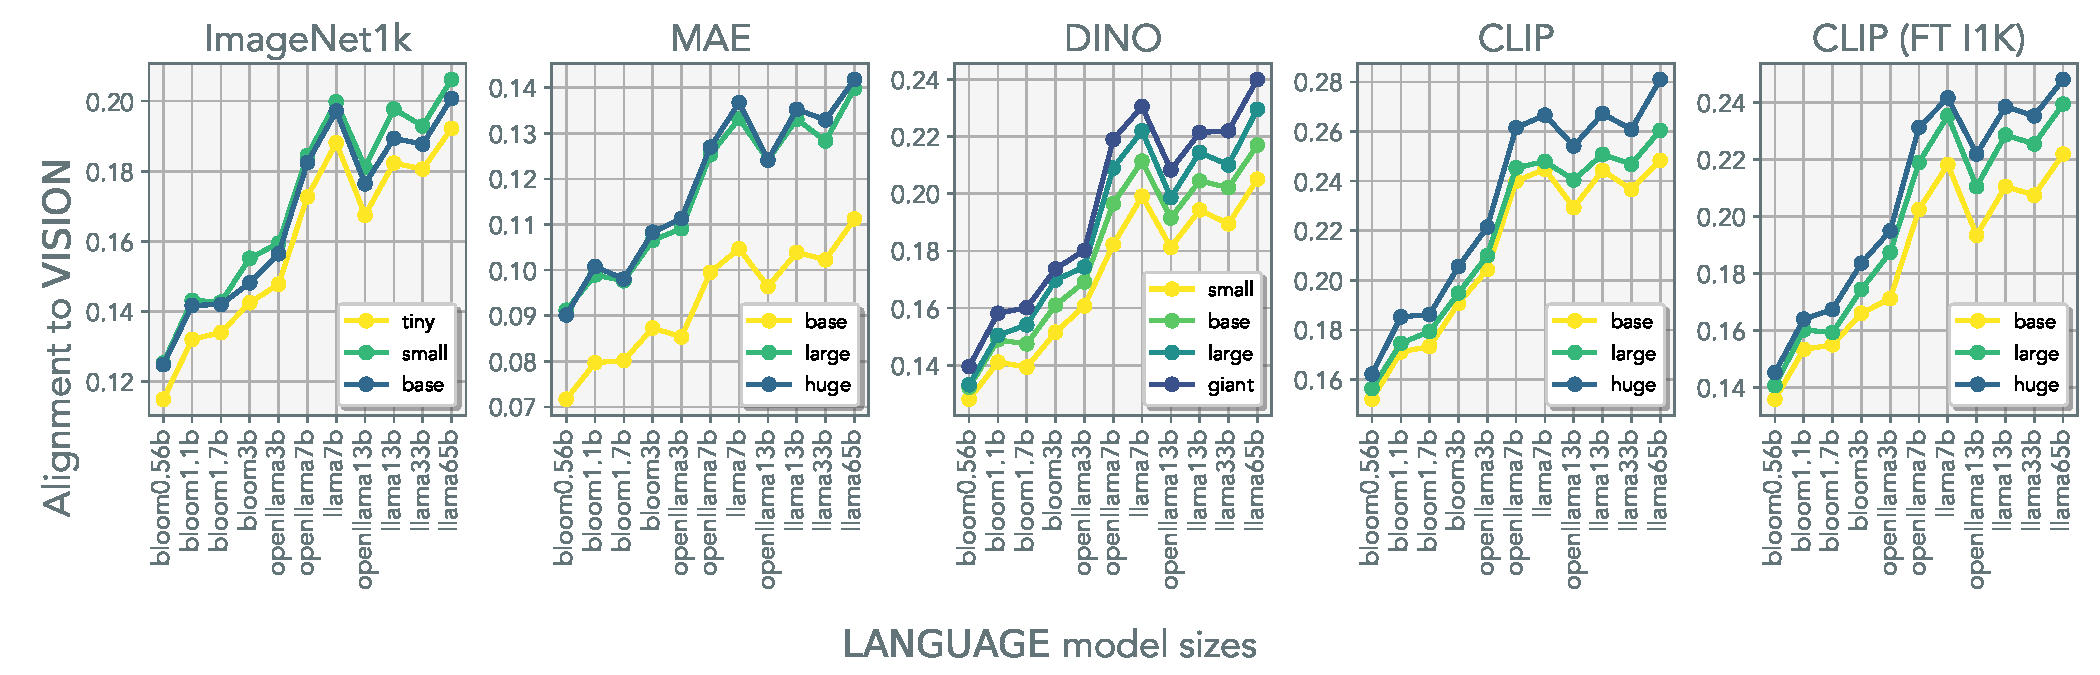
\includegraphics[width=1.\linewidth]{figures/llm_alignment_per_task.pdf}\\[-0.1in]
%     \caption{\small \textbf{LANGUAGE models align with VISION:} We measure the alignment of language models to vision models for each vision task. Language models are ordered by size. Alignment is a measure of the mutual nearest-neighbor on Wikipedia caption dataset (WIT). For most tasks we see a consistent trend, larger language models are more aligned with vision models.}
%     \label{fig:llm2lvm_align}
% \end{figure*}
% \begin{figure*}[t!]
%     \centering
%     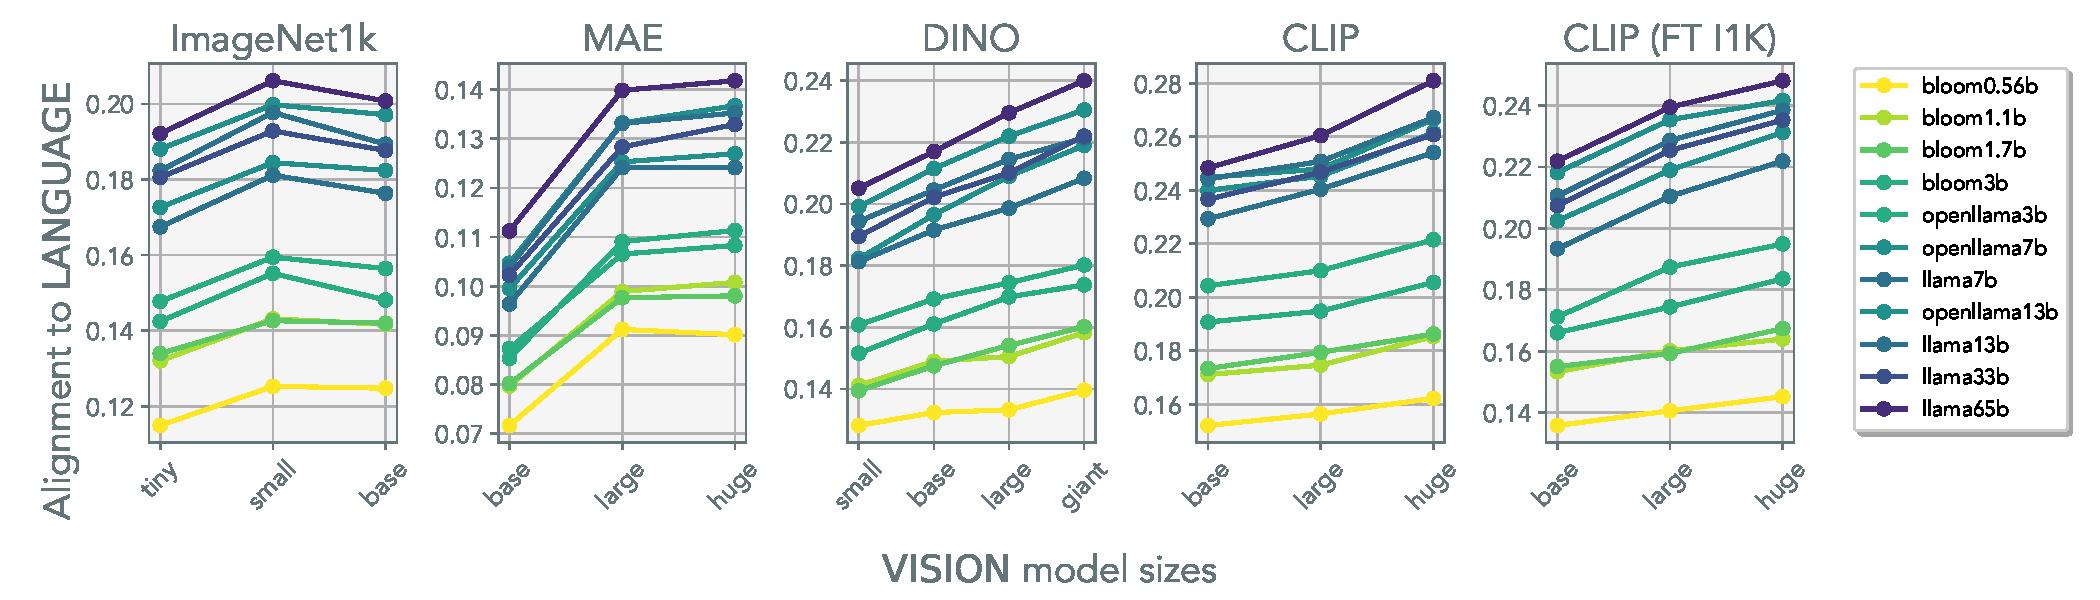
\includegraphics[width=1.0\linewidth]{figures/lvm_alignment_per_task.pdf}\\[-0.1in]
%     \caption{\small \textbf{VISION models align with LANGUAGE:} We measure the alignment of vision models to language models. Alignment measures are grouped for each vision task. Vision models are ordered by size and measure the mutual nearest-neighbor on Wikipedia caption dataset (WIT). The figures shows a consistent trend of larger vision models align more with larger language models.}
%     \label{fig:lvm2llm_align}
% \end{figure*}

\begin{figure*}[t!]
    \centering
    % \subfigure[\textbf{LANGUAGE models align with VISION.} Language models are ordered by size.]{
    %     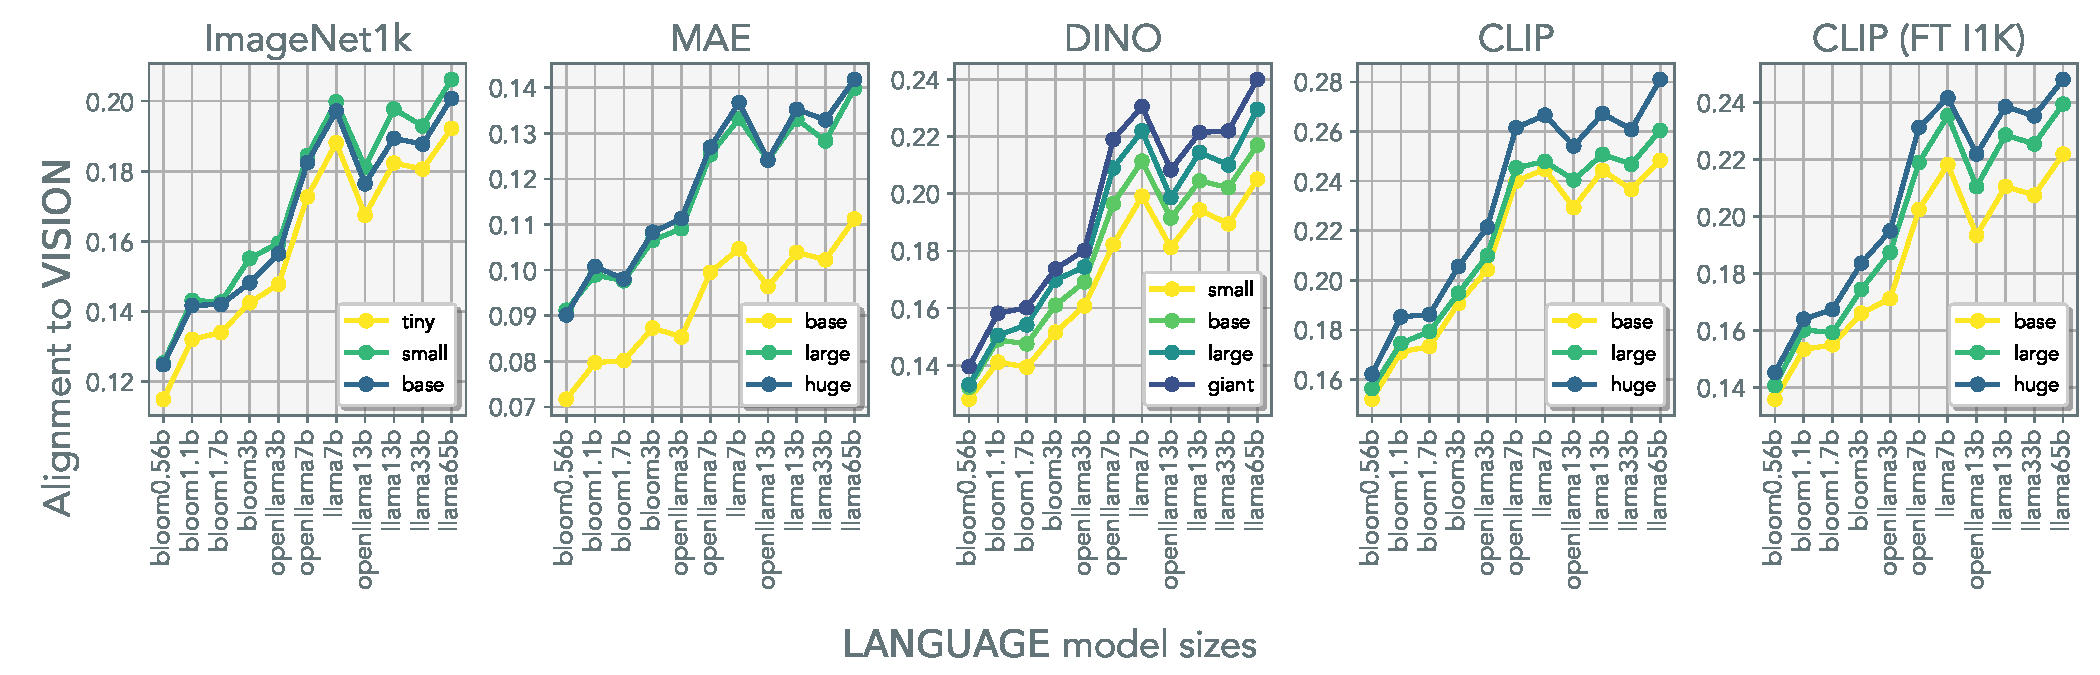
\includegraphics[width=1.0\linewidth]{figures/llm_alignment_per_task.pdf}
    %     \label{fig:llm2lvm_align}
    % }\\[1pt] % Adjusted spacing
    
    % \subfigure[\textbf{VISION models align with LANGUAGE.}  Vision models are ordered by size.]{
    %     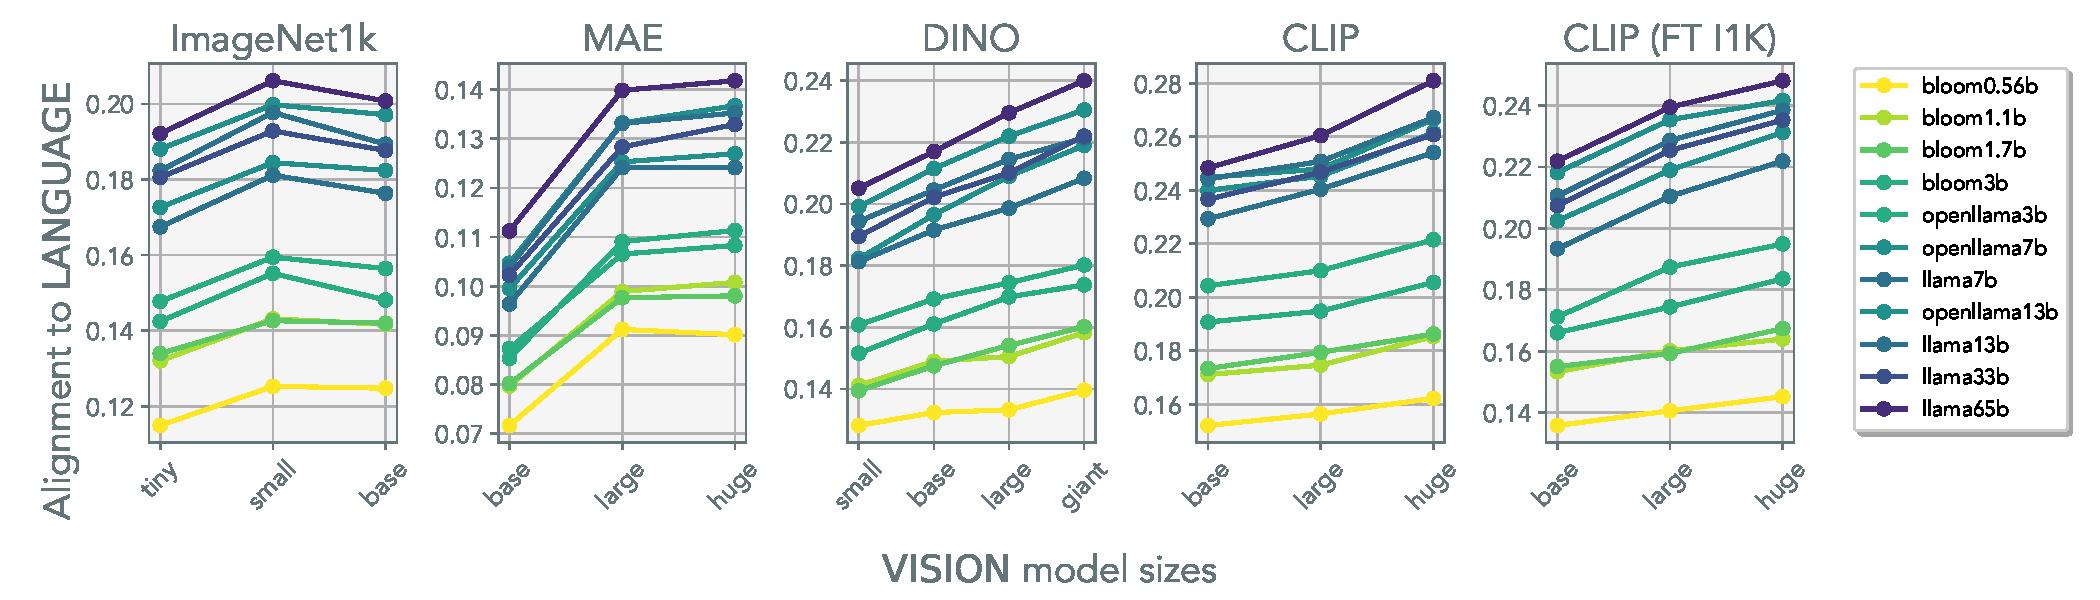
\includegraphics[width=1.0\linewidth]{figures/lvm_alignment_per_task.pdf}
    %     \label{fig:lvm2llm_align}
    % }\\[-7pt]
    % \vspace{-1pt}
    % 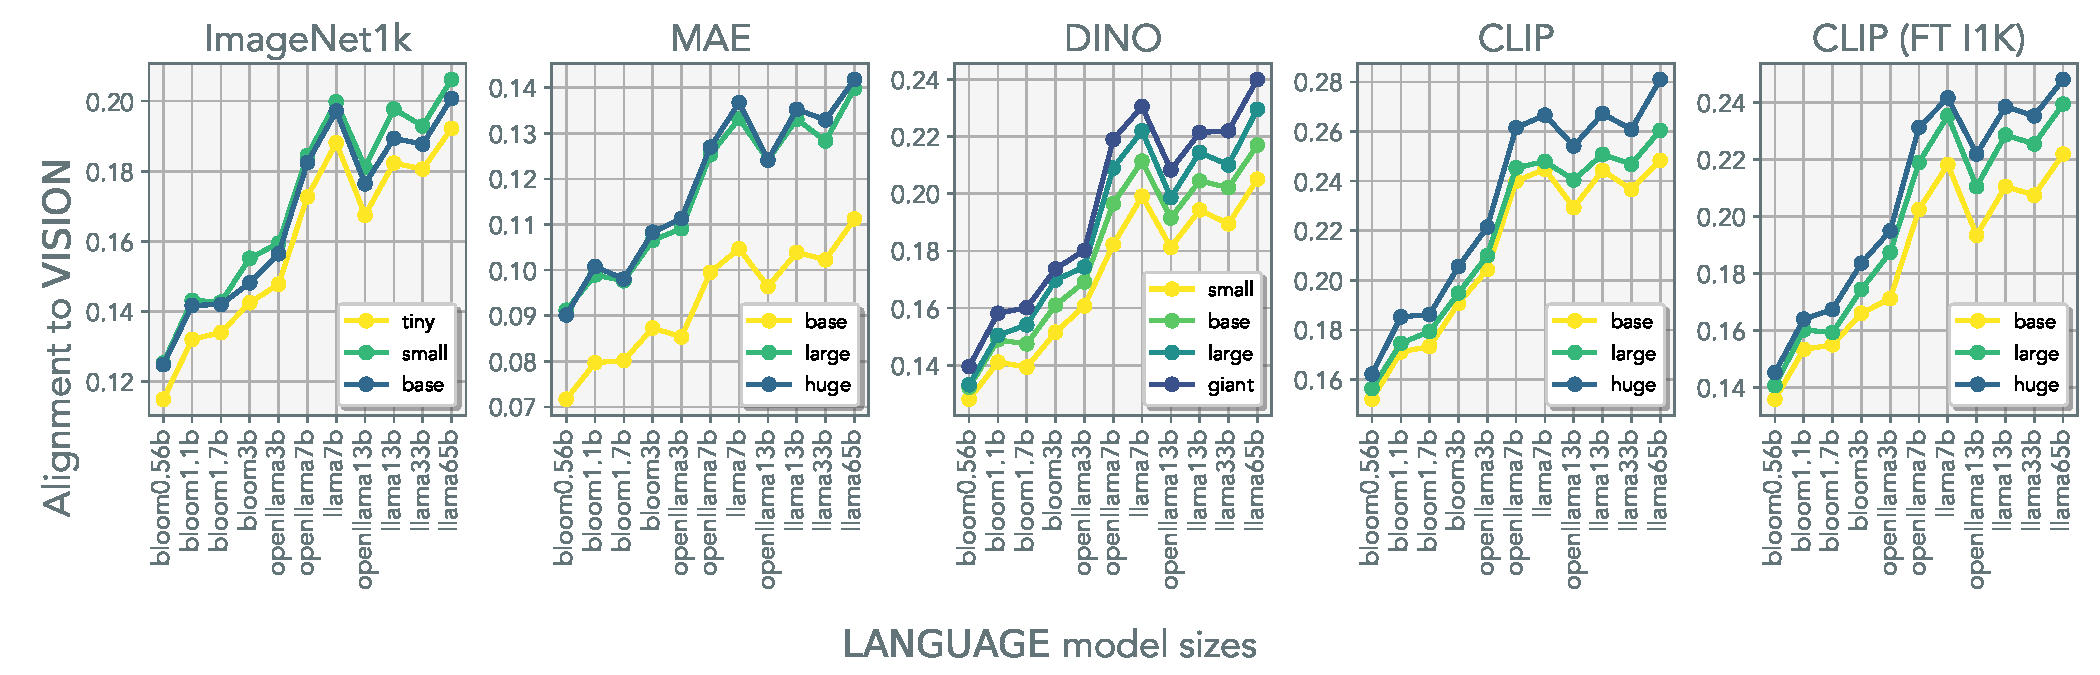
\includegraphics[width=1.0\linewidth]{figures/llm_alignment_per_task.pdf}\\[2pt]
    % 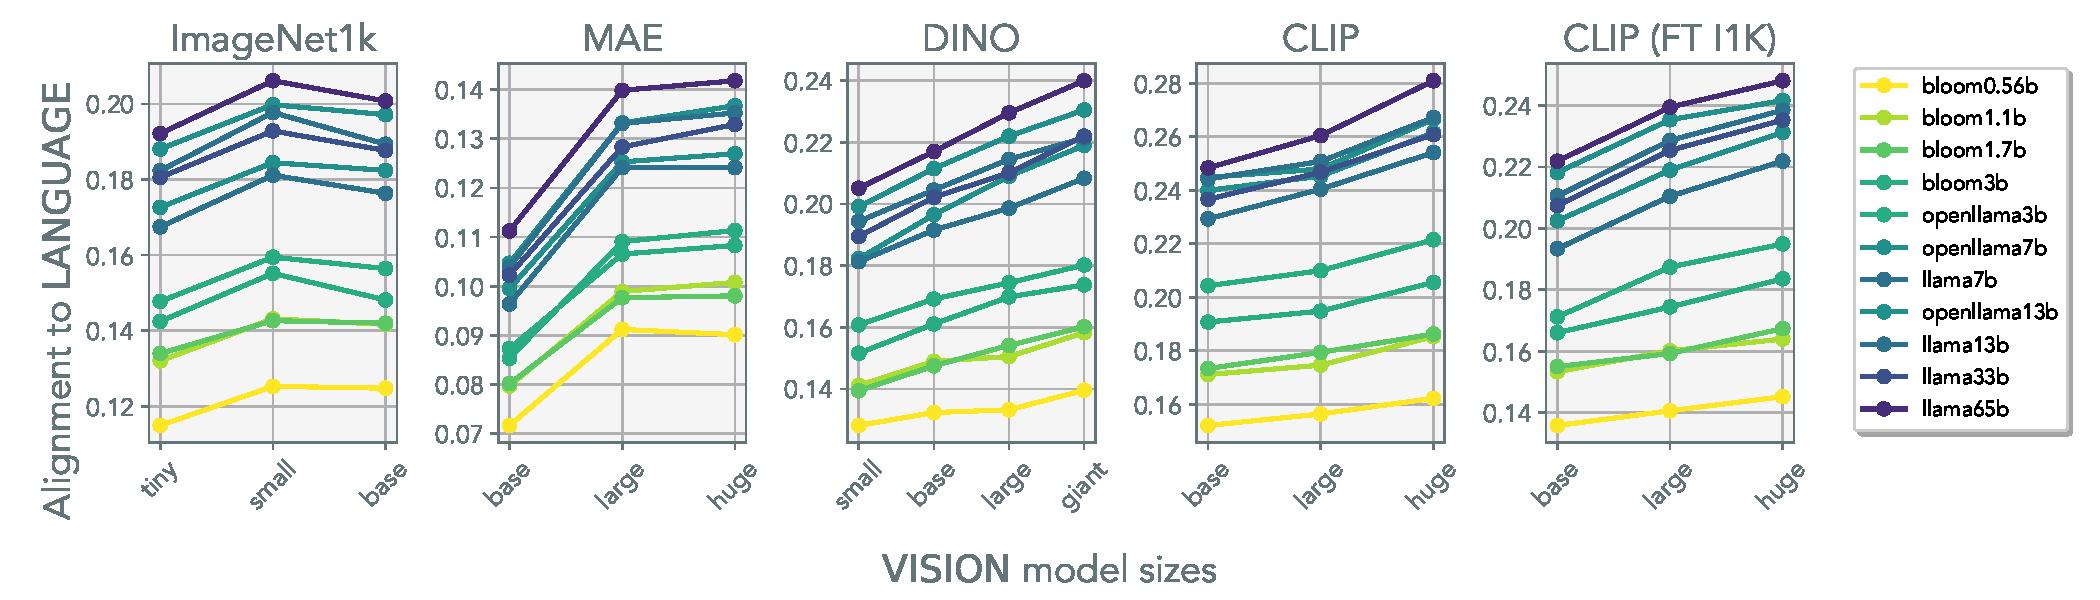
\includegraphics[width=1.0\linewidth]{figures/lvm_alignment_per_task.pdf}
    % % \label{fig:lvm2llm_align}
    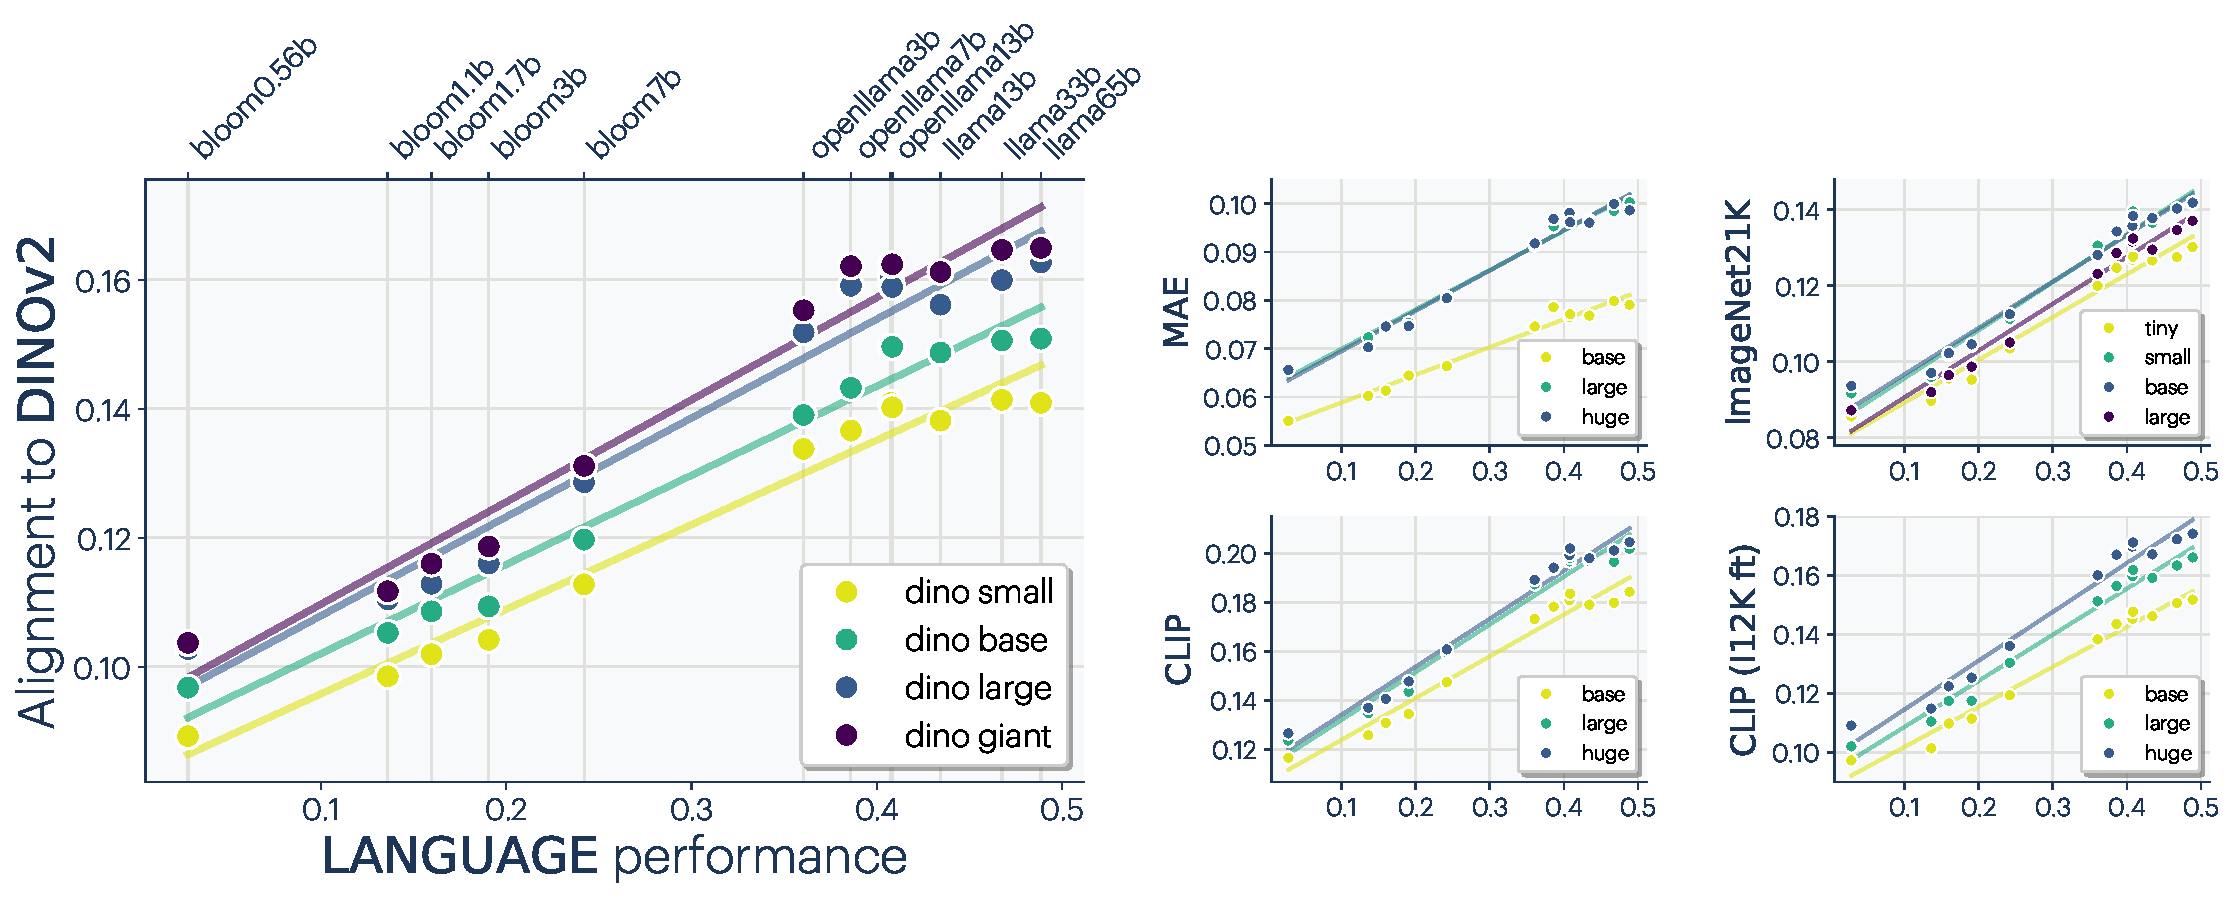
\includegraphics[width=1.0\linewidth, trim=0 0 0 16]{figures/llm_to_vision_ppl.pdf}
    \vspace{-22pt}
    \caption{\small\textbf{LANGUAGE and VISION models align:} 
    We measure alignment using mutual nearest-neighbor on the Wikipedia caption dataset~(WIT)~\cite{srinivasan2021wit}. The x-axis is the language model performance measured over 4M tokens from the OpenWebText dataset~\cite{Gokaslan2019OpenWeb} (see \app{app:other-metrics} for plots with model names). 
    We measure performance using $1 - \texttt{bits-per-byte}$, where $\texttt{bits-per-byte}$ normalizes the cross-entropy by the total bytes in the input text string.
    The results show a linear relationship between language-vision alignment and language modeling score, where a general trend is that more capable language models align better with more capable vision models. 
    We find that CLIP models, which are trained with explicit language supervision, exhibit a higher level of alignment. However, this alignment decreases after being fine-tuned on ImageNet classification (labeled CLIP (I12K ft)).
    }%
    \label{fig:alignment_comparisons}
    \vspace{-4pt}
\end{figure*}

\subsection{Alignment increases with scale and performance}

\citet{kornblith2019similarity} and \citet{roeder2021linear} observed model alignment not only exists but also increases with model scale and dataset size. On CIFAR-10 classification, \citet{krizhevsky2009learning} found that larger models exhibit greater alignment with each other compared to smaller ones. 
Theoretically, \citet{balestriero2018spline} showed that models with similar outputs (\eg, as a result of having high performance) also have similar internal activations. 
% \citet{roeder2021linear} further demonstrated that, under the same objective, increasing model capacity and dataset size leads to convergent representations.
With the continuing trend of models scaling up, this suggests model alignment will increase over time -- we might expect that the next generation of bigger, better models will be even more aligned with each other.% should be more aligned with each other.
%
% \phil{Tongzhou's results here}

We expand upon this observation by evaluating the transfer performance of $78$ vision models. These models were trained with varying architectures, training objectives, and datasets~(detailed in~\Cref{sec:vision-vision-details}). In~\Cref{fig:vm_align} (left), we bin these models based on their average transfer performance on the VTAB dataset~\cite{zhai2019vtab}, and then measure the average kernel alignment of the models within each bin. % $m_{\texttt{NN}}$.
The results indicate that models with high transfer performance form a tightly clustered set of representations, while models with weak performance have more variable representations. We further visualize this structure with UMAP~\citep{mcinnes2018umap} over models representation in~\Cref{fig:vm_align} (right). This suggests that models that are competent all represent data in a similar way. Echoing \citet{bansal2021revisiting} and \citet{tolstoy1877anna}, we might say: all strong models are alike, each weak model is weak in its own way. 

% Moreover, we believe that convergence increases as models become more competent.
% In \Cref{fig:vm_align}, we evaluate alignment among $77$ vision models of different architectures, trained with different objectives and datasets. Alignment is significantly higher among models that are more capable at solving a general set of downstream tasks. 

%\citet{moschella2022relative} found that different architectures and/or different objectives and/or different datasets, can arrive at the same representation up to an affine transform.

%\citet{klabunde2023similarity} also found that.

%Such representations in some models have aligned to the point where it becomes difficult to identify between these models in domains like neuroscience \cite{han2023system}. %This might not be surprising. After all, we have established that different model representations converge to biological representations, and argued for this from the intelligence perspective, \emph{i.e.}, a ``necessity driven by intelligence'' \Cref{sec:models-and-minds}.  In this section, we take a machine learning perspective and discuss how the very setting for learning these models (that is parametrizations, data, optimizations, etc.) can suggest such a convergence of different types of models -- in essence, all roads lead to Rome~\citep{bansal2021revisiting}.


%Next we move on to indirect measures. If models $f_A$ and $f_B$ are aligned, then we might expect that subcomponents of $f_A$ can be stitched together with subcomponents of $f_B$, with minimal adaptation.



%\paragraph{Model averaging and stitching}
% \jh{likely due to LMC, models can be easily averaged or stitched. These models can be arbitrarily stacked because they have converged to shareable and similar representations.}



% the practice of model stitching, averaging, and ensemble methods align with the concept of representational convergence in deep networks. The combination of different models through stitching or averaging leverages their shared functional characterizations, leading to improved performance. Ensemble methods, including averaging models within an ensemble, further emphasize the convergence of representations by utilizing the collective knowledge learned by multiple models. These techniques provide compelling evidence that models can converge towards similar representations, contributing to the overall understanding of representational convergence in deep learning.
%In conjunction with the observation that large models are mode-connected, came the investigation of averaging models. Not only has it been shown that models can be averaged with negligible interference but often can be used to congregate and learn better model representations.

%Averaging models have also proven to be a powerful technique for improving performance. \cite{wortsman2022fi,wortsman2022model,jolicoeur2023population} demonstrated that averaging models lead to better outcomes. 

% So far we have argued that different models are converging on the same representation (distance function). Are they also converging on the same weights? Well obviously not for models with different weight spaces, but there is some evidence that models initialized from the same weights often converges on the basin~\cite{wortsman2022model}.
% % Even with different initializations solutions for the same model are permutations of each other. 
% Even with different initialization, solving for permutation and merging models has shown promise in enhancing performance~\cite{ainsworth2022git}.
% Recent advances have further improved permutation and merging techniques, as demonstrated in the works of~\cite{stoica2023zipit,jordan2022repair}.

%\bc{Not sure what the below is meant to convey? Do we want to take the position that generative models is more ideal for convergent representations than others? This is kind of my takeaway from this paragraph below}
%Further evidence of convergence can be found in the literature on generative models. The probability distribution $P(X)$, of the total data $X$, is a sufficient statistic for any statistical inference that can be made from the data X \phil{say this more precisely} \cite{XX}. Perhaps because of this property, generative models have long been considered the ``ultimate'' data representation \cite{XX,YY,ZZ}. With the recent advent of highly capable generative models for images, language, and other domains, many works have shown that these models can be adapted to performing numerous tasks beyond just making up random content. \citet{luo2023readout} show that a diffusion model of images can be adapted to perform many standard computer vision tasks. ... This is basically the foundation model argument we mentioned above, except now we are saying that th particular kind of foundation model that is highly compelling is a generative one. The others, we argue, are just small transformations of the generative model. It all comes back to the platonic model $P(X,Y)$.

The discussion so far indicates that various models are aligning toward a unified representation. But does the convergence extend to model weights? While models with different architectures might not have compatible weight spaces, there exists ample evidence that models with the same architecture will often converge to the same basin of weights~\cite{nagarajan2019uniform,garipov2018loss,lubana2023mechanistic}. This holds even for models with different initializations, up to permutations over weight space~\citep{ainsworth2022git}. Because of this, it is possible to merge separately trained models of the same architecture, and achieve some of the capabilities of all models in the mixture~\cite{stoica2023zipit,jordan2022repair,wortsman2022model}.
% \citet{wortsman2022model, BLA, BLA, BLA} empirically observed the tendency for models to gravitate towards the same `basin` and use it too.
%Even when models begin with different initialization, they can end up in 

%solving for permutations over weight space allows models to be merged into a single set of weights that can , obtaining the functional capabilities of all merged models ~\citep{ainsworth2022git,stoica2023zipit,jordan2022repair,wortsman2022model}.
% (the merged model can obtain functional capabilities of both the merged models). 

% \jh{not sure where this should go. i dont think it belongs in multi-modal section. putting it here for now.}
% However, model-alignment has not been a universal opinion. \citet{bender2020climbing} famously argued that LLMs are not grounded, and without grounding they only will acquire a superficial understanding of the world. This argument was expanded into the Stochastic Parrots hypothesis. Others have presented evidence to the contrary: LLMs do achieve these various kinds of grounding. Word2vec and Tegmark showed they get representations of space and time.


%Ensemble methods, which involve averaging multiple models, have also been extensively studied. \cite{huang2017snapshot,izmailov2018averaging} explored the effectiveness of averaging models within an ensemble. The benefits of averaging have long been established, as demonstrated by~\cite{polyak1992acceleration}.
%Moreover, the use of an average model as a target has been investigated by~\cite{tarvainen2017mean,cai2021exponential,grill2020bootstrap}. These works highlight the advantages of incorporating averaging techniques into the learning process.

% In conclusion, the practice of model stitching, averaging, and ensemble methods align with the concept of representational convergence in deep networks. The combination of different models through stitching or averaging lxeverages their shared functional characterizations, leading to improved performance. Ensemble methods, including averaging models within an ensemble, further emphasize the convergence of representations by utilizing the collective knowledge learned by multiple models. These techniques provide compelling evidence that models can converge towards similar representations, contributing to the overall understanding of representational convergence in deep learning.

% \paragraph{Further discussion} % change title later or move to conclusion

% Every new sample point is an observation that sheds light on the underlying processes of the world. Each additional piece of data inevitably shapes the trajectory of the model's hypothesis about the world. To put this in the parlance of deep learning, this evolving theory is the representation that the model learns from the data.
% While it's true that various representations may explain the same dataset, the volume of plausible hypotheses can only decrease as more data is observed. Ultimately, the representation with the highest predictive capacity that accommodates future observations outshines its counterparts.

% In homage to Newton-Smith's argument for convergent realism, it's important to note that the representation itself and the mechanistic process that led to these representations may undergo significant shifts over time. Yet, even in the face of such paradigm shifts and scientific revolutions, the representational power of these models is destined to improve. Indicating that despite the ebbs and flows of theoretical development, there remains constant progress toward better model representations.

% \section{These trends can be explained by scale}

% There are many reasons why we might see such a convergence: perhaps it's a social effect, where different communities talk more and all intellectual diversity collapses, or perhaps it is because we all use the same hardware, and the hardware determines properties of the representations \cite{hardware lottery}.

% In this section, we point out a third possibility: models scale over time, and the larger the scale the greater the convergence.

% To test this hypothesis, we run the following experiments. We define three kinds of scale: model parameter count, training data size, training flops. Functions of these attributes are commonly called scaling laws. Here we present a scaling law of representational alignment. For each scale variable, we create 10 evenly spaced bins. Then we plot \texttt{CKA} alignment within each bin. The results are shown in figures XX, YY, and ZZ.

% Scale explains the trends to a similar degree as time did. Could it be that time is causal and scale simply correlates with time. If we look within a single year, holding time constant, we see the same effect of scale, as shown in figure XX. If we instead hold scale constant, the effect of time is much diminished. Therefore, we conclude that scale is a better explanation of the trends we are seeing.

% \subsection{Why does scaling lead to convergence}

% This is expected if the thing we are converging to is the solution to an optimization problem with a single global minimum\footnote{Or multiple minima that all induce the same distances~\cite{permutation invariance works}.}. Then if you optimize better (via scaling), of course you converge.


% \subsection{Convergence of abstractions}
% \bc{This section needs citations}

% % Generative models learn latent representations that act like graphics primitives -- lights, camera angle, consistent geometry, etc. We conjecture that this is because both are models of physics, and lights, cameras, and geometry are ``true'' properties of the physical world. All reasonable models will converge on these truths.

% Physical laws govern our world. These laws are not initially known by humans, but some have been gradually discovered over thousands of years. 
% %Since ancient times, philosophers and scientists have come up with hypotheses that potentially explain certain observed phenomena (such as the rise and the fall of the sun), gather new data in experiments to verify or falsify their hypotheses, and eventually converge on certain explanations (such as the rotation of the earth) \citep{newton1989truth}. 
% To explain the observed phenomenon, we developed an understanding of something that is not (as easily and directly) observable. These observations are distilled into abstractions, which are promoted to the level of laws because they survive and remain consistent after repeated counterfactual and adversarial testing.
% % \jh{Is there a compression argument here? The minimal length description of the observations is the physical laws that governs them. Any description that is smaller is either wrong or identical, and the previous description was verbose.}

% Similar to humans, certain artificial models also explain certain observations of the real world. Through a similar process of repeated testing in the optimization and compression, artificial models must also develop abstractions of their observations. Generative neural networks are artificial models trained to \emph{model} a certain part of the real world, \textit{\eg}, 2D photos of objects. After training on a dataset of samples, without supervision on how the world works, they can be used to generate synthetic 2D images that look just like a real photo, 
% % or short stories that read like they are from human writers, 
% or even effective chemical molecules. Such models have displayed a strong capability to produce believable samples, but do they really understand the data they are approximating? Do artificial models understand the optical process that governs how a photo is captured? Do they understand the chemical reactions among different molecules? The answer, we argue, is \emph{yes}. While current artificial systems do not perform their experimentation or counterfactuals, their learning operates under the same constraints as the abstractions and physical laws we develop. Namely, every representation generated (i.e., abstraction) by the model must fit as many observations as possible (i.e., have high fitness). 
% % Optimization processes like stochastic gradient descent act as the repeated testing that their representations are subjected to. 
% But without the agency of creating its own counterfactuals, this learning has the limitation of only being able to explain existing observations. Though as these models interact more with the real world in a more autonomous fashion, a growing fraction of the observations they learn from will be from their own actions.

% When fit to 2D images, generative models have shown an emergent understanding of the 3D structures, light transport, or temporal effects of the underlying physical world, even though they are never trained on these structures. In particular, such models disentangles properties like \emph{3D rotation angle}, \emph{object size}, and \emph{color} as controllable knobs \citep{jahanian2019steerability}. For a generated image of an object, one can tune these knobs to \emph{independently} control the corresponding properties. In other words, by just learning to generate 2D images, the model develops an understanding of the underlying physical structures. 


% \tz{
% identifiability?
% }

% \section{Representational convergence of models}

% The alignment of model and human representation, as revealed empirically, prompts the question of whether models themselves are converging. Architecturally, this convergence has been apparent. Innovations such as residual connections, weight-reuse, attention mechanisms, and transformers being universally adopted across various tasks and sensory modalities. 
% Such generalist architecture components have proven to yield little to no performance loss over their specialist counterparts. They are increasingly adopted over the machine learning community due to their capability, versatility, and usefulness in multi-task multi-modal models. While these are likely not at the very ``optimality'', the ongoing convergence to such general-purpose architectures components is evident.


% Another critical aspect of convergence has emerged in the form of representational convergence. Here, representational convergence pertains to the concept that models progressively align toward the same functional characterization of the data. We discuss several threads on the topic of representational convergence.
% %As a disclaimer, we are not concerned with how we have arrived at the same representation or whether these models have learned the same mechanistic decision processes. Indeed, it's essential to acknowledge that not every domain within the field has undergone through this ``representational convergence'', a topic we will delve into subsequently.



%\subsection{Convergence of models and minds} \label{sec:models-and-minds}

%The human brain has five canonical modalities to experience the world. These sensory modalities are the only functional inputs of the external world to the brain. With the rapid development and distribution of the computer screen, the sense of vision has become the dominant modality in which we organize and communicate our knowledge due to its scalability. Capable of being recorded, replicated, and transmitted over large distances makes vision noticeably more efficient to distribute throughout human ecosystems than the other senses. Furthermore, considering that about thirty percent of the primate brain is dedicated to visual processing, it makes sense as the modality of choice for studying the inputs to intelligence.

%From this perspective, it may not be as surprising that the vision modality became one of the earliest successes for the development of compelling artificial intelligence models that rely on adapting to large volumes of data \cite{krizhevsky2017imagenet, russakovsky2015imagenet}. And as a reflection of the amount of biological relevance present in this data, the representations that emerge in these artificial models are similar to those in human and animal brains. We conjecture that the models are trained on similar data and tasks as humans were trained/evolved on \cite{yamins2014performance}. More recently, the similarities have expanded beyond visual perception; artificial models have had significant success in abstractions beyond the sensory input, such as language \cite{schrimpf2021neural, zhang2019bertscore}.

%LPIPS and perceptual alignment papers. In LPIPS we found that if you train a net on any of a variety of tasks -- supervised, self-supervised, etc -- it learns to measure distances in a way that correlates with how humans perceive perceptual similarity.

%objective (and data) affect alignment \citep{muttenthaler2022human}
%BERT features correlate w human \citep{zhang2019bertscore}

%\bc{Not sure if this next paragraph fits in with the rest:}
%The study of artificial intelligence has led to remarkable discoveries, particularly in visual perception and language processing. Interestingly, the evolutionary path of biological systems and our artificial technology have resulted in striking similarities, despite their vastly divergent developmental trajectories. For instance, artificial models optimized for mapping visual percepts to language (\eg segmentation, detection, whole-image classification) all appear to reach a common solution. Stepping back, the task space between these mappings may also be converging when you consider the scope of broader datasets. Segmentation, detection, and whole-image classification are problems with differing spatial granularity.

\begin{figure*}[ht]
    % \vspace{-3pt}
    \centering
    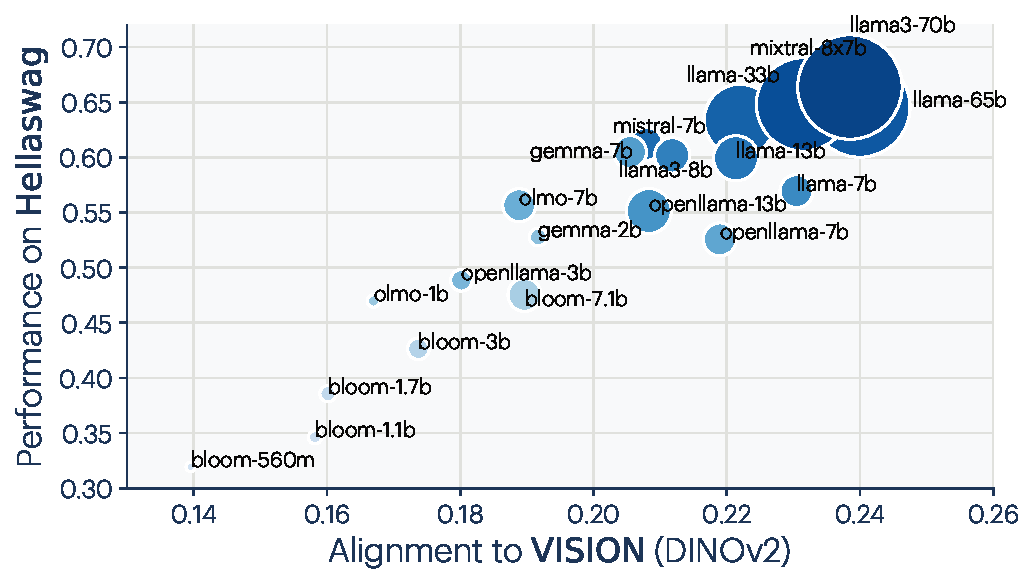
\includegraphics[width=0.5\linewidth]{figures/alignment_hellaswag.pdf}%
    \hfill%
    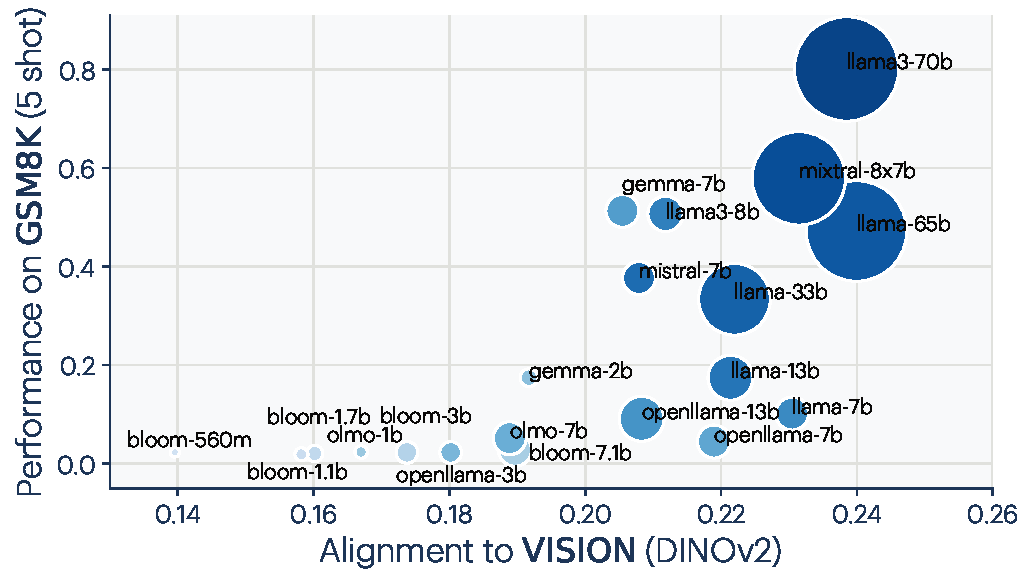
\includegraphics[width=0.5\linewidth]{figures/alignment_gsm8k.pdf}\\[-0.15in]
    \caption{\small\textbf{Alignment predicts downstream performance:} We visualize correlation between LLM alignment score to DINOv2~\cite{oquab2023dinov2} and downstream task performance on Hellaswag~(common-sense)~\cite{zellers2019hellaswag} and GSM8K~(math)~\cite{cobbe2021gsm8k}. LLMs are plotted with radii proportional to the size of the model, and color-coded by their rank order in language modeling scores ($1 - \texttt{bits-per-byte}$). We observe that models aligned more closely with vision also show better performance on downstream language tasks. For Hellaswag, there is a linear relationship with alignment score, while GSM8K exhibits an ``emergence''-esque trend. 
    } 
    \label{fig:downstream}
    % \vspace{-5.5pt}
\end{figure*}


% \subsection{Representations are converging across data modalities}
\subsection{Representations are converging across modalities}
% Language-vision models often start with a pretrained language model and stitch it to a pretrained vision models. This is the case for Llava, etc. This suggests that a lightweight interface can align the two representations in the two pretrained models. Boaz Barak et al. investigated this further and found that it holds.
Do models trained on different data modalities also converge?
%Alignment of models occurs beyond its own modality. 
%\citet{merullo2022linearly} extend the observation of model alignment to cross-modal data:
Several works indicate that the answer is \emph{yes}. 

\citet{merullo2022linearly} extended model stitching to the cross-modal setting, finding that a single linear projection is sufficient to stitch a vision model to an LLM and achieve good performance on visual question answering and image captioning. \citet{koh2023grounding} showed that linear stitching can also work in the opposite direction, aligning text inputs to visual outputs. 
%stronger vision models stitched with an LLM perform better on VQA and image captioning tasks. 
In fact, many recent language-vision models stitch pre-trained language and vision models together. For example, LLaVA~\cite{liu2023llava} demonstrated state-of-the-art results by projecting visual features into a language model with a 2-layer MLP.
%\citet{koh2023grounding} showed that language models can process and produce visual data by operating on linearly transformed visual representations.

Other works show further kinds of evidence of cross-modal synergy. \citet{achiam2023gpt} found that jointly training a language model with a vision model improves performance on language tasks, compared to training the language model on its own. \citet{sorscher2022neural} show a setting in which word embeddings of visual concept names can be isometrically mapped to image embeddings for those same concepts. In work concurrent to ours, \citet{maniparambil2024vision} show well-trained vision encoders on large datasets exhibit high semantic similarity with language encoders regardless of the training paradigm (supervised, self-supervised, or language-supervised). \citet{sharma2024vision} probed the visual knowledge of LLMs trained \textit{only} on language data, by converting images into code that an LLM can process. They found that LLMs have rich knowledge of visual structures, to the extent that decent visual representations can be trained on images generated solely by querying an LLM to produce code and rendering the response. In visual generation, LLMs show abilities to augment captions with visual structures (\eg, bounding boxes) and improve generation quality \citep{betker2023improving,lian2023llm,lian2023llmvideo,wu2023self}. Over other modalities, \citet{ngo2024language} showed auditory models are also roughly aligned with LLMs up to a linear transformation, and \citet{ng2023can} demonstrated the effectiveness of using pre-trained LLMs for facial motion prediction.

We set out to address these claims in a broader scope to determine whether models are indeed learning an increasingly modality-agnostic representation of the world. We sampled a variety of models trained either solely on vision or solely on language, and compared their representations as they became larger and more competent over many tasks.


% First, to measure alignment, we use the nearest-neighbor metric on paired caption data, a choice based on the limitations of existing metrics like CKA~\cite{kornblith2019similarity} and SVCCA~\cite{raghu2017svcca}. These metrics have a stricter definition alignment, which may not fit our current needs. 
% For instance, understanding the precise relationship between unrelated items, such as an apple and Bill Gates, or the exact distances among a dog, a cat, and a bowl of cereal, may not be critical. It's more important to recognize that a dog and cat are likely to co-occur than either is to a cereal bowl.

% For similar reasons, existing works relied on alternative metrics such as model-stitching as it
% ``reveals aspects of representations that measures such as centered kernel alignment (CKA) cannot''~\cite{bansal2021revisiting}. However, for billion parameter models, this becomes quickly infeasible to scale, and we have opted for a simpler metric of mutual nearest-neighbors~\cite{klabunde2023similarity}. Given an image-text pair $(x_{\mathsf{image}}, x_{\mathsf{text}})$, we pass image $x_{\mathsf{image}}$ through vision model and $x_{\mathsf{text}}$ through the language model and measure its intersection of neighbors. A greater overlap between the neighbor sets implies better alignment between the models. Although mutual nearest-neighbor has its own quirks and issues, we use it as proxy for examining alignment between vision and language models. Further investigation is needed to identify a more accurate metric for alignment measurement. See~\app{sec:alignment_methods} for further details and discussion.


%We now put our hypothesis to test. 
In~\Cref{fig:alignment_comparisons}, we assess alignment between a suite of language models and vision models. So far we have only defined alignment for two kernels defined over the same input space. To measure cross-modal alignment, we use paired datasets to bridge the two modalities. For vision and text, we use the Wikipedia captions dataset $\{(x_i, y_i)\}_i$~\cite{srinivasan2021wit}, composed of images from Wikipedia ($x_i$) and their corresponding captions ($y_i$). We then measure alignment between a language model $f_{\texttt{text}}$ and a vision model $f_{\texttt{img}}$ as the alignment of the two following kernels:
\begin{align}
    K_\texttt{img}(i, j) = \langle f_{\texttt{img}}(x_i), f_{\texttt{img}}(x_j) \rangle\\
    K_\texttt{text}(i, j) = \langle f_{\texttt{text}}(y_i), f_{\texttt{text}}(y_j) \rangle.
\end{align}
% This allows us to measure the similarity between $K_\texttt{img}$ and $K_\texttt{text}$ with standard metrics. 
% $f_{\texttt{img}}$ and $f_{\texttt{text}}$ are both transformer models in all our experiments. We extract the class tokens from the vision models and the average-pooled tokens from the language models to obtain our vision and language embeddings. We pick the layer to extract these tokens from by finding the setting that maximizes alignment. We measure alignment using our mutual nearest-neighbor metric with $k=10$. 
%If two models measure distance between corresponding samples in similar ways~(\ie respective kernels), we say that they have aligned representations. 
% The horizontal axis in \Cref{fig:alignment_comparisons} represents language model performance. 
Using this analysis, we find that the better an LLM is at language modeling, the more it tends to aligns with vision models, as shown in \Cref{fig:alignment_comparisons}. The converse effect also holds: the better a vision models is, the more it tends to align with LLMs. See \Cref{sec:vision-language-details} for more details.
% Conversely,~\fig{fig:alignment_comparisons} measures alignment from the opposite perspective, examining how vision models align with language models. Here, we observe that the larger the vision model, the higher the alignment with language models (across a range of LLM scales). 
%Additionally, we observe that the level of alignment is also sensitive to task and to who trained these models, suggesting that differences in other training details 
%(optimization methods, dataset size, etc) also influence alignment. Despite these nuances, the consistent trend across our results is that the larger the vision model, the more aligned it will be with language representations, and vice versa.%the platonic representation hypothesis, particularly in the context of multi-modality. 
% Further experiments on different datasets are detailed in~\app{}.

%In \Cref{sec:what-why-converge}, we will turn our attention to our hypotheses as to why this convergence is happening.

%The average \texttt{CKA} between models is increasing over time. This is true for both vision models and for language models: in each subsequent year, two given vision models will tend to measure distance between images in more and more similar a way, and similarly for language models for distance between text. 
%Remarkably, we also observe a cross modality convergence: the \texttt{CKA} between vision models and language models is also increasing over time.





% \begin{figure}
%     \centering
%     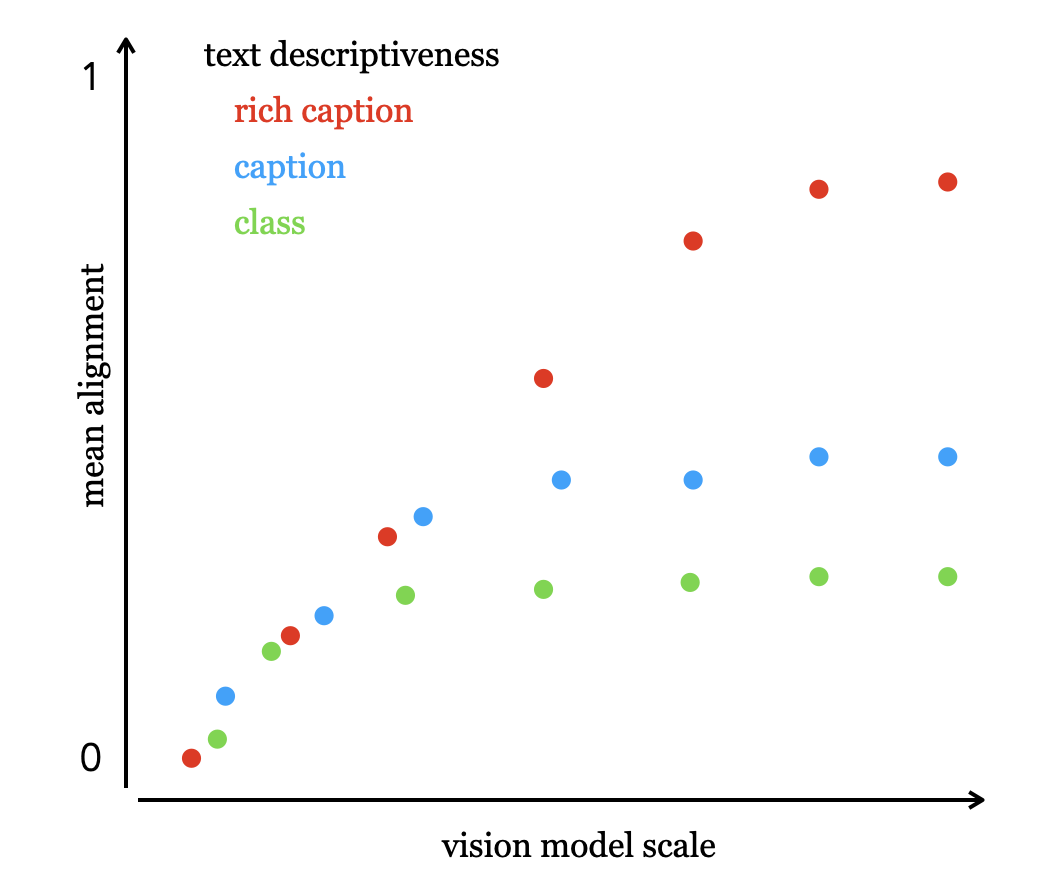
\includegraphics[width=1.0\linewidth]{figures/richness.png}
%     \caption{Richness.}
%     \label{fig:richness}
% \end{figure}



% Therefore, we conclude that our feeling is valid: over time, models, within and between modality, are measuring distance between items in more and more similar ways.


\subsection{Models are increasingly aligning to brains}
\label{sec:models-and-minds}

Neural networks also show substantial alignment with biological representations in the brain~\cite{yamins2014performance}. This commonality may be due to similarities in the task and data constraints both systems are confronted with.
%likely stems from the universal underpinnings of information processing. 
Even though the mediums may differ -- silicon transistors versus biological neurons -- the fundamental problem faced by brains and machines is the same: efficiently extracting and understanding the underlying structure in images, text, sounds, \etc~\cite{barlow1961possible, olshausen1997sparse}. \citet{sorscher2022neural} developed a theoretical framework for how the efficient extraction of novel concepts occurs for both the human visual system and deep networks. The tasks that the human visual system has been honed to perform through evolution -- like segmentation, detection, and whole-image classification -- are also the ones that we train our neural nets to perform. \citet{yamins2014performance} went as far as to title their work in the spirit that performance over such tasks implies brain alignment. \citet{antonello2024predictive} posited that it is less the particular task and more the generality of the representations that explain their alignment with biological representations. Further, \citet{conwell2022can} showed that training data plays a large role in alignment. Psychophysical studies have also shown agreement between how humans perceive visual similarity and how models do, even when the models are trained on tasks, such as self-supervised prediction, that are seemingly unrelated to mimicking human perception~\cite{zhang2018unreasonable}.%Model representations have become so aligned amongst each other that models are difficult to tell apart in data regimes relevant to neuroscience \cite{han2023system}.
%Moreover,~\citet{han2023system} observed that many modern neural nets exhibit similar representations, making it hard to distinguish one model from another using standard neuroscience techniques.
% are so similar to on another that current techniques used in neuroscience can struggle to distinguish one model from another ~\cite{han2023system}.\jh{the last sentence feels like an overly strong statement?}
%The commonality in representations among many different AI models to the brain has reached a point where identifying architectural features using current similarity metrics has become surprisingly difficult~\cite{han2023system}.

%This phenomenon provides a potent testament to the robustness and adaptability of computational principles and the possibility of reaching similar solutions to the same problems, regardless of the substrate in which the computation is performed.


\subsection{Does alignment predict downstream performance?}
If models are converging towards a more accurate representation of reality, we expect that alignment should correspond to improved performance on downstream tasks. \Cref{fig:downstream} supports this hypothesis by demonstrating improved performance on commonsense reasoning (Hellaswag; \citet{zellers2019hellaswag}) and mathematical problem solving (GSM8K; \citet{cobbe2021gsm8k}) as alignment improves. %This downstream task correspondence on common sense and math reasoning provides evidence that the representational convergence we observe does indeed reflect models learning increasingly accurate representations of the underlying reality that enables such reasoning capabilities.

\section{Why are representations converging?}\label{sec:what-why-converge}

% This sections outlines our main arguments for the hypothesis that mode


Modern machine learning models are generally trained to minimize the empirical risk with possible implicit and/or explicit regularization: \begin{equation*}
    {
    \color{gray}
    \overbracket[1pt]{\color{black}f^*}^{\mathclap{\textsf{trained model}}}
    }{}= \mathbox[model]{\argmin}_{f \in {
    \color{gray}
    \underbracket[1pt]{\scriptsize\mathbox[model]{\color{black}\mathcal{F}}}_{\mathclap{\scriptstyle\textsf{function class}}}}
    }\mathbb{E}_{x \sim {\scriptsize\mathbox[task]{\mathsf{dataset}}}}[ {
    \color{gray}
    \overbracket[1pt]{\mathbox[task]{\color{black}\mathcal{L}}}^{\mathclap{\textsf{training objective}}}}(f, x)] + {
    \color{gray}
    \underbracket[1pt]{\mathbox[bias]{\color{black}\mathcal{R}}}_{\mathclap{\textsf{regularization}}}}(f)
\end{equation*}
In the following sections, we lay out how each colored component in this optimization process potentially plays a role in facilitating representational convergence. % we consider the role of each colored component in how different models learn converging representations.

\begin{figure*}[t]
    \centering
    \vspace{3pt}
    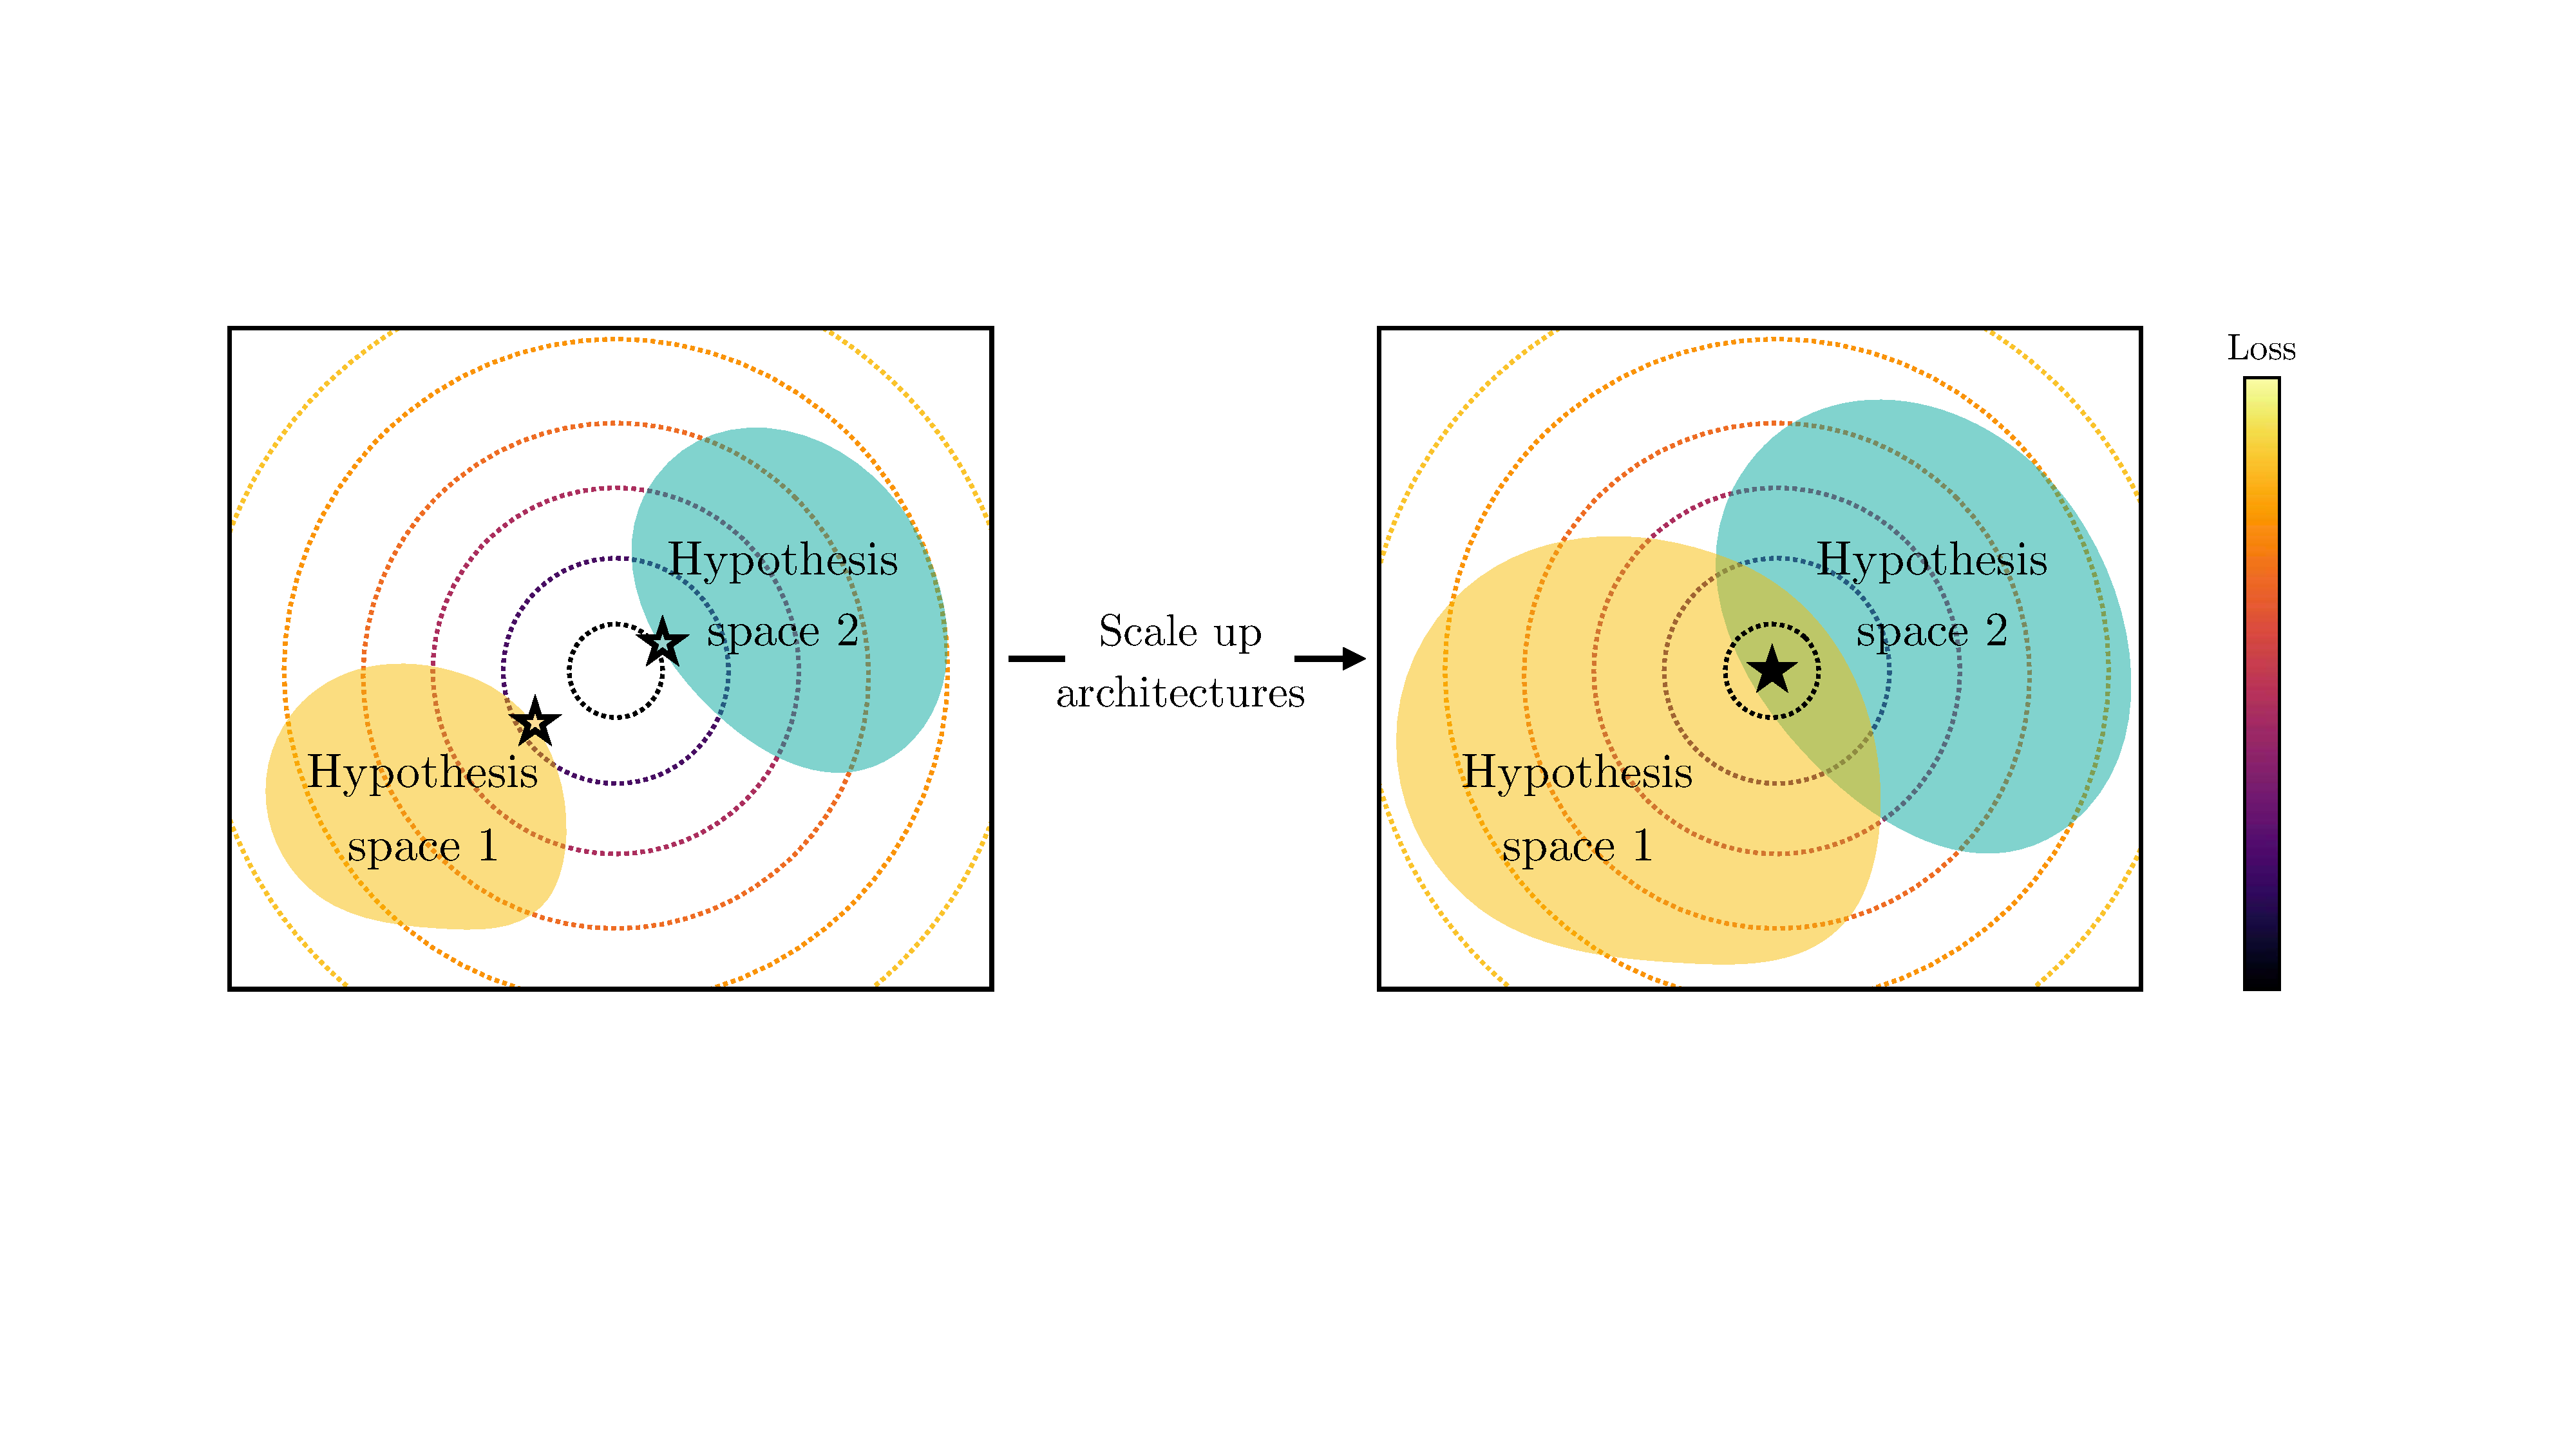
\includegraphics[width=0.945\linewidth, trim=0 0 12 0]{figures/hypothesis_space_overlap.pdf}\\[-8pt]
    \caption{\small \textbf{The Capacity Hypothesis:} If an optimal representation exists in function space, larger hypothesis spaces are more likely to cover it. \textbf{LEFT:} Two small models might not cover the optimum and thus find \textit{different} solutions (marked by outlined \scalebox{1.25}{$\bigwhitestar$}). \textbf{RIGHT:} As the models become larger, they cover the optimum and converge to the same solution (marked by filled \scalebox{1.05}{$\bigstar$}).}
    \label{fig:hypothesis_space_overlap}%
    \vspace{-5pt}
\end{figure*}

\begin{figure}[t]
    \centering
    \vspace{3pt}
    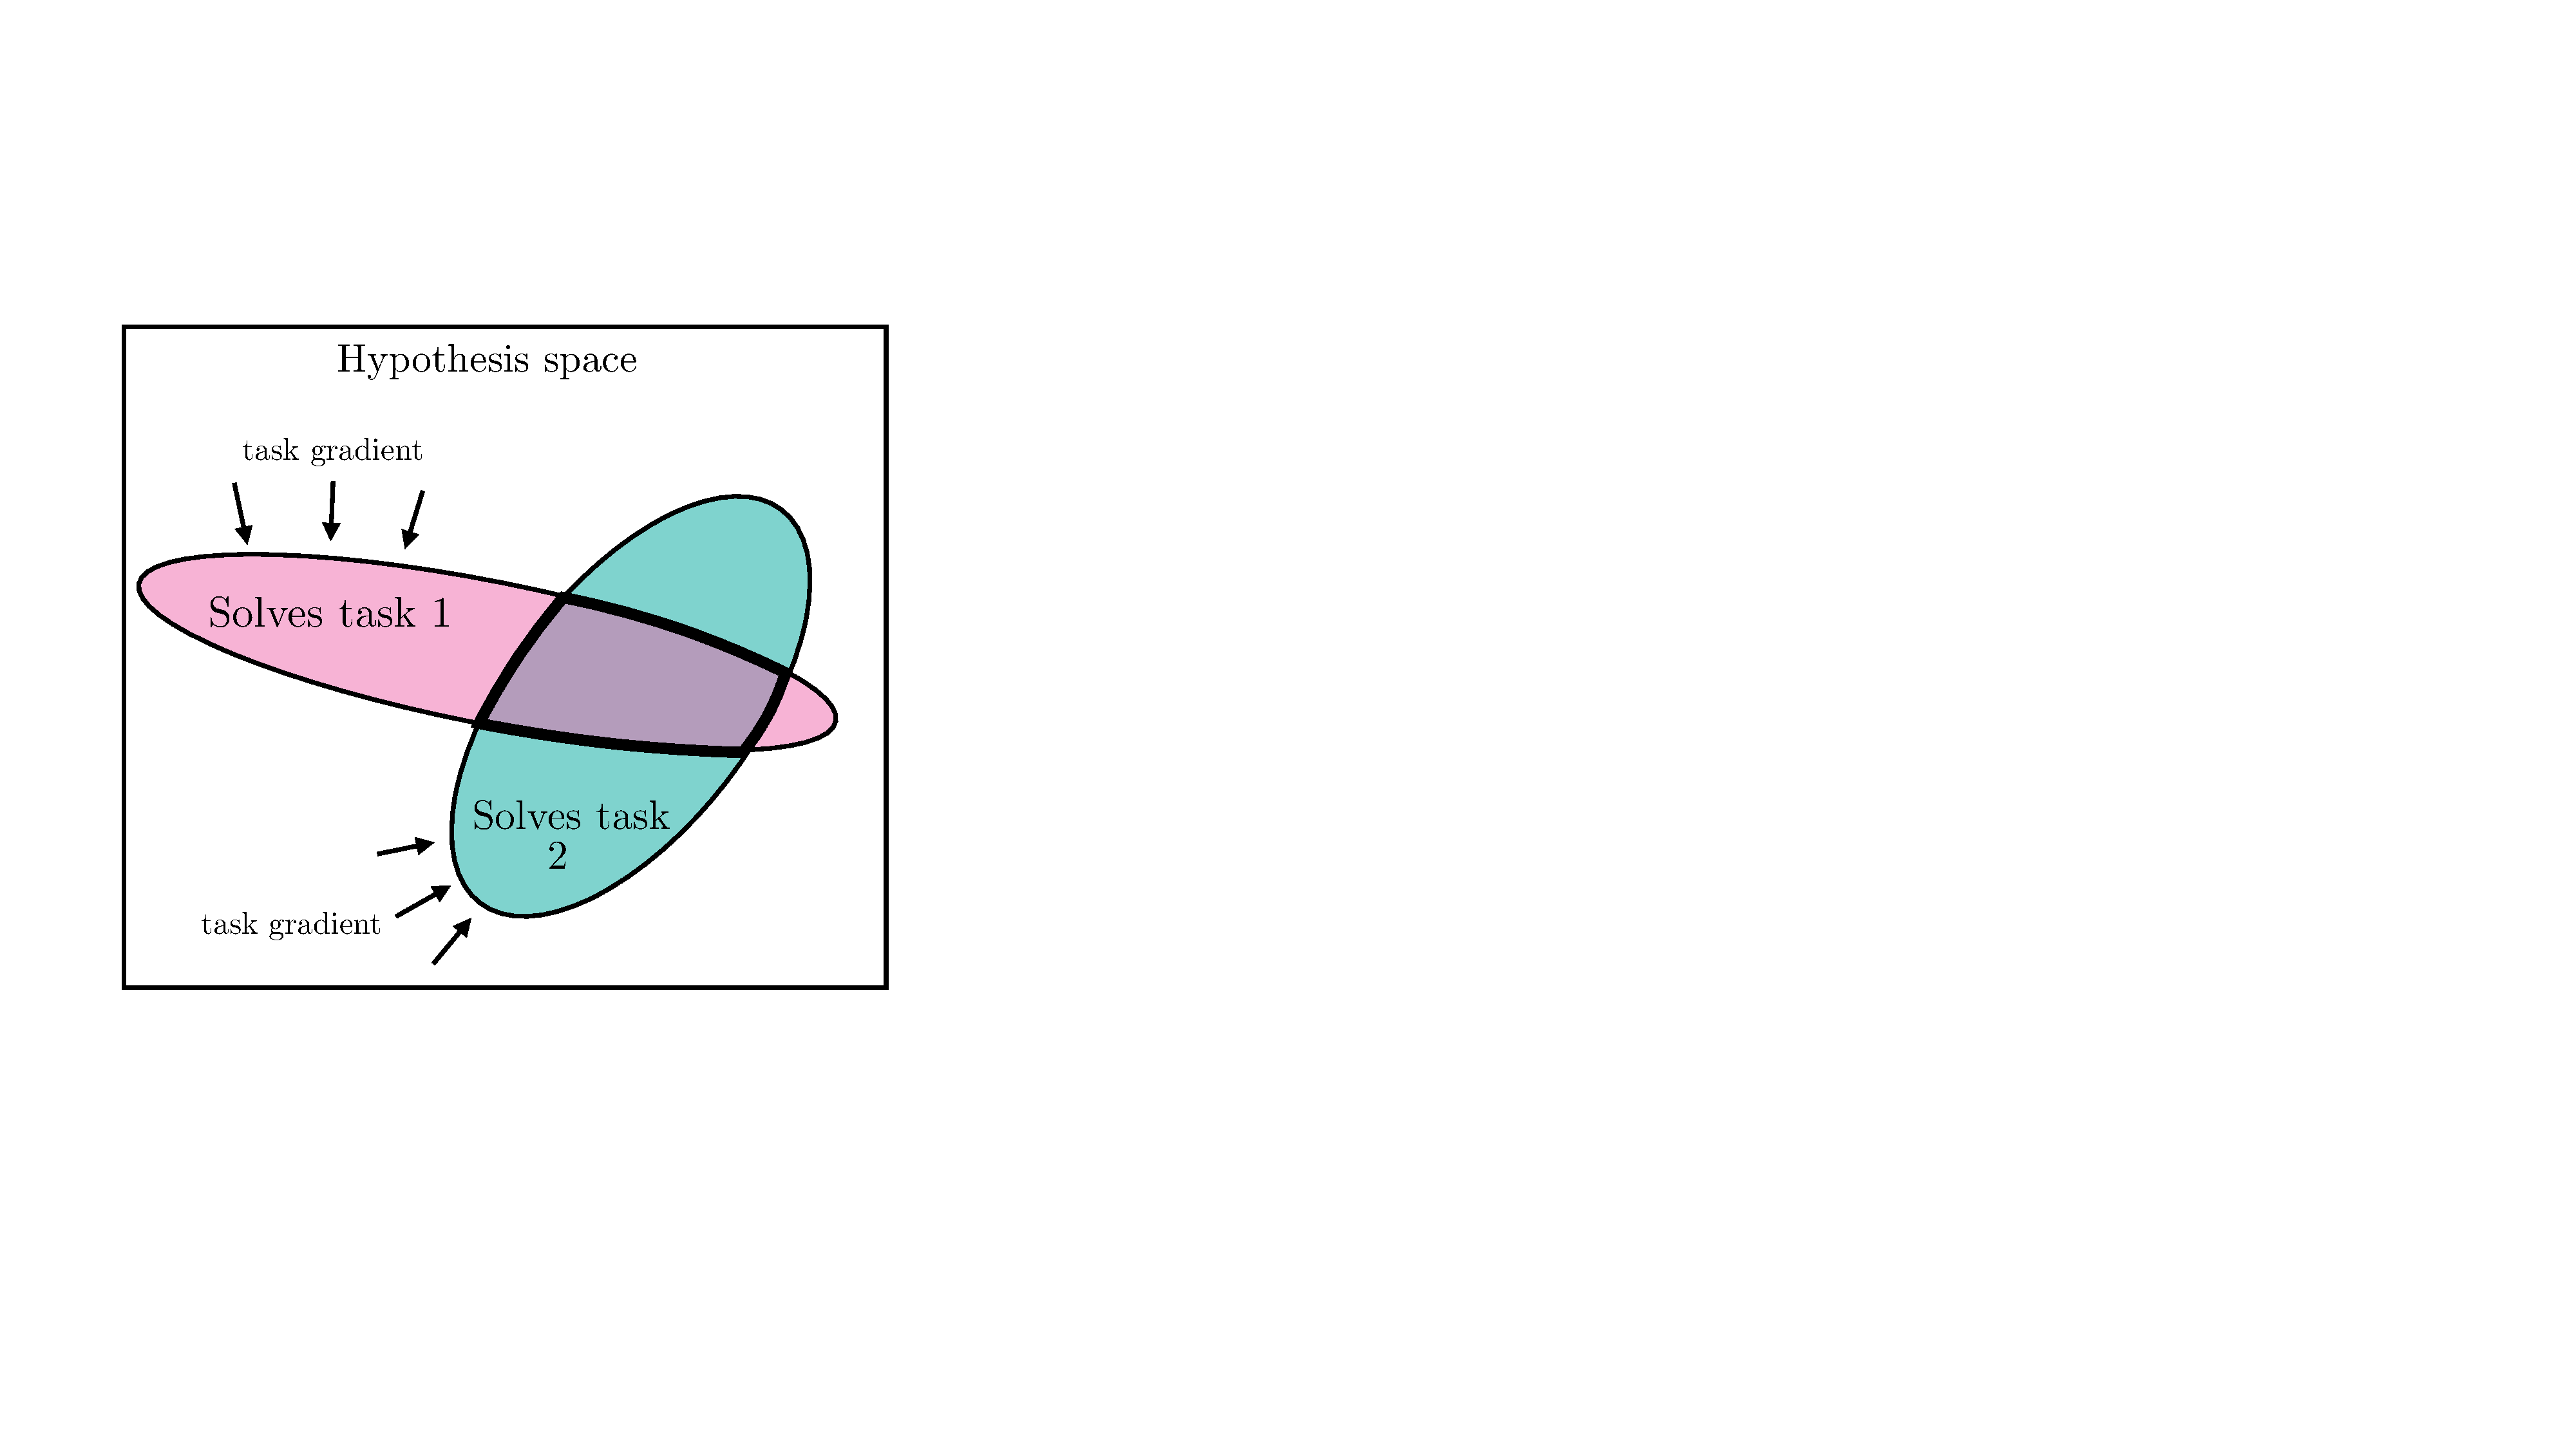
\includegraphics[width=0.825\linewidth]{figures/multitask_hypothesis.pdf}\\[-7pt]
    \caption{\small \textbf{The Multitask Scaling Hypothesis:} Models trained with an increasing number of tasks are subjected to pressure to learn a representation that can solve all the tasks.} \label{fig:multitask_hypothesis}
    % \vspace{1pt}
\end{figure}

% \subsection{Convergence via \colorbox{green!30}{Task Generality}}
\subsection{Convergence via \textbox[task]{Task Generality}}
\label{sec:multitask_scaling_hypothesis}
% \vspace{-1pt}

%\paragraph{Scaling Law: Solution Convergence from Big Data}
% \jh{big models scale predictably with params. Bigger models require less and less fine-tuning.}
% The increasing prominence of deep learning models has drawn attecntion to the financial incentives associated with large models. 
% Scaling up models has become a central focus for those wishing to obtain performance regardless of efficiency of the algorithm itself. With the cost of amassing data and training these models continues to rise, there is a strong interest in understanding how models scale with parameters.

Each training datapoint and objective (task) places an additional constraint on the model. As data and tasks scale,
% With more data points, 
the volume of representations that satisfy these constraints must proportionately grow smaller, as visualized in Figure \ref{fig:multitask_hypothesis} and stated below: 
\hypbox{The Multitask Scaling Hypothesis}{%
There are fewer representations that are competent for $N$ tasks than there are for $M<N$ tasks. As we train more general models that solve more tasks at once, we should expect fewer possible solutions.
}

This has been previously termed as the Contravariance principle by~\citet{cao2021explanatory}, which states that the set of solutions to an easy goal is large, while the set of solutions to a challenging goal is comparatively smaller. Moreover, we argue that this narrower solution set also generalizes better. As data scales, models that optimize the empirical risk $\mathbb{E}_{x \sim {\scriptsize \mathbox[task]{\mathsf{dataset}}}}[ {{{\mathcal{L}}}}(f, x)]$ also improve on the population risk $\mathbb{E}_{x \sim {\scriptsize \mathbox[task]{\mathsf{reality}}}}[ {{{\mathcal{L}}}}(f, x)]$, and become better at capturing statistical structures of the true data generating process ($\mathsf{reality}$).
% its fixed, trying to make the color box rounder but it seems to break inside equation
%As data scales, models that optimize the empirical risk (loss over samples) also improve on the population risk (loss over the full data generating process).

% In other words, the size of the set of optima or solutions is contravariant with the difficulty of the optimization problem. Hence, with increased scale of data, given the same algorithmic family (\eg, transformer trained with SGD), there exists a correspondence between a model's representational capacity (\eg parameter count) and generalizing capabilities where the loss of a model's given presentation provides an accurate ranking of it's generalization capabilities relative to other models.


%This study of how a model behaves with scale is referred to as a scaling law. Scaling laws study how a model's in- and out-of-domain generalization changes with data and parameter size. 
%The first work can be dated back to \citet{cortes1993learning}, which has been revisited by \citet{hestness2017deep} for the modern deep learning era. Since then, scaling laws have emerged as a fundamental area of interest, leading to numerous follow-up studies that attempt to uncover the equations governing scaling laws through empirical measurements~\cite{rosenfeld2019constructive,kaplan2020scaling,hoffmann2022training}. 
% So far there has not been any work demonstrating how to modify the exponent of the power law within the family of deep neural networks optimizing on natural data. Understanding the power law within the context of the scaling law remains an active area of research, with some initial studies investigating scaling laws in the context of kernels~\cite{bahri2021explaining}. 

Recent work has demonstrated a power law relationship between data scale and model performance~\cite{hestness2017deep}. This implies that with enough data (\eg, consisting of the entire internet and all offline scientific measurements) one ought to converge to a very small solution set with irreducible error -- the inherent epistemic uncertainty of the world. 
% While the internet is only a carefully curated snapshot of human civilization
As more models are trained on internet-scale data, the set of solutions that satisfies all data constraints must become relatively small. 
%Where within one of these solutions is the true reflection of the universal physical laws governing the reality that data originally manifested from. 


In addition to data-scaling, many modern representation learning objectives $\mathbox[task]{\mathcal{L}}(f, x)$ directly optimize for multi-task solving. Contrastive learning finds a distance structure over data samples that optimizes many classification tasks \citep{arora2019theoretical,tongzhouw2020hypersphere,tian2020rethinking}. Masked Autoencoders \citep{he2021masked} optimize randomly sampled reconstruction tasks. In fact, autoregressive language modeling can also be seen as optimizing a diverse set of tasks \citep{radford2019language}. Such multi-task objectives may be more effective than single-task ones (\eg, ImageNet classification) due to the fact that they impose more task constraints on the representation, leading to a smaller and higher-quality solution space \citep{chen2020simple,he2020momentum,radford2017learning,radford2019language}.

% \begin{tcolorbox}[colback=white!95!black,colframe=white!30!black]
% \textbf{The Scaling Hypothesis} 
% \\
% \\
% Corollary of multitask hypothesis.
% \end{tcolorbox}




% However, this idealized analysis has its limits, especially when considering lossy observation functions. Despite these limitations,

% the model is believed to encapsulate essential aspects of more complex, real-world systems. This analysis offers a pathway towards understanding the essence of what representations converge to, supporting the hypothesis that learning systems are moving towards a unified model, proficient across various domains and modalities, fundamentally grounded in the cooccurrence of events.


\subsection{Convergence via \textbox[model]{Model Capacity}}\label{sec:capacity_hypothesis}

% \fixme{data to task sec}

Suppose there is a globally optimal representation for standard learning objectives. Then, under sufficient data, \textit{scaling} a model (\ie, using larger function classes 
\mathbox[model]{\mathcal{F}}), as well as \textbox[model]{improved optimization}, should be more effective at finding better approximations to this optimum, as illustrated in \Cref{fig:hypothesis_space_overlap}. 
% As any two hypothesis spaces grow, they should both find better and increasingly similar approximations.
% there is a greater chance of the overlap containing the optimum of the ambient function space (since the region of overlap becomes strictly larger).
% Especially with the increased scale of data, given the same algorithmic family (\eg, transformer trained with SGD), there exists a correspondence between a model's representational capacity (\eg, parameter count) and generalizing capabilities where the loss of a model's given presentation provides an accurate ranking of its generalization capabilities relative to other models. 
% Scaling width and depth increases the network capacity, and thereby improves its ability to approximate the optimum. And better optimization helps the learning process find this approximation.
With the same training objective, larger models, even of different architectures, will thus tend to converge toward this optimum. When different training objectives share similar minimizers, larger models are better at finding these minimizers, 
and will train to similar solutions over the training tasks. We summarize this hypothesis as follows:
% \jh{should we make a distinction between generalization and optimization? }
\hypbox{The Capacity Hypothesis}{%
Bigger models are more likely to converge to a shared representation than smaller models. 
}
%A set of big models is more likely to have an overlapping hypothesis space than a set of small models. When hypothesis spaces overlap, then there is the possibility for convergence.

% Scaling data makes the empirical risk a better approximation to the population risk; the empirical risk introduces random variable due to data sampling, which is removed in the population risk, and therefore optimizing the population risk will necessarily result in greater alignment than optimizing empirical risk. Scaling training time results in the model converging to its training minimizer; that is, different optimization trajectories become aligned to the global minimizer of the training loss.

% The situation for scaling model size is shown in figure \ref{fig:hypothesis_space_overlap}.



\subsection{Convergence via \textbox[bias]{Simplicity Bias}}\label{sec:simplicity_bias_hypothesis}
% \jh{algorithmic bias towards converging towards simple functions}


Arriving at the same mapping on the \textit{training data} does not prohibit the models from developing distinct internal representations. It is not unreasonable to posit that the representations used to detect a dog in a 1M parameter model could be quite different than that used by a 1B parameter model. What would stop a billion-parameter (and counting) model from learning an overly complicated and distinct representation? One key factor might be simplicity bias:

\hypbox{The Simplicity Bias Hypothesis}{
Deep networks are biased toward finding simple fits to the data, and the bigger the model, the stronger the bias. Therefore, as models get bigger, we should expect convergence to a smaller solution space.}

% How does solution convergence relate to representational convergence? Indeed, there are many ways for a neural network to represent a solution function, and not all such ways have the same representation. 

% In practice, neural network models are \emph{optimized} via learning algorithms. Representational convergence can be influenced by the learning algorithm itself. The inductive biases of gradient descent have demonstrated a tendency to converge towards low-rank parameters ~\cite{gunasekar2018implicit,arora2019implicit}.
% Recent research has built upon these findings and argued for a convergence towards low-rank functional mappings~\cite{valle2018deep, huh2023simplicitybias,dingle2018input}. These works observed that there is relative increase in the volume of simple and low-rank functions as the depth of these networks become deeper. \jh{add more relevant works}. 

% \fixme{a few sentences about explicit regularization}

% We argue that neural networks are biased towards find simple solutions, and 
% Explicit regularization terms $\mcolbox{red!30}{\mathcal{R}(f)}$ are often used to 
\vspace{2pt}
Such simplicity bias could be coming from explicit regularization $\mathbox[bias]{\mathcal{R}(f)}$ commonly used in deep learning (\eg, weight decay and dropout). However, even in the absence of external influences, deep networks naturally adhere to Occam's razor, \textbox[bias]{implicitly favoring simple solutions}that fit the data~\cite{solomonoff1964formal,gunasekar2018implicit,arora2019implicit,valle2018deep, huh2023simplicitybias,dingle2018input, goldblum2023no}. 
%While this does not always guarantee deterministic convergence towards the same generalizing properties for two models~\cite{liu2020bad}, with a sufficiently large dataset, it's natural to suspect that these models are more likely to converge towards similar representations. 
Figure \ref{fig:simplicity_hypothesis} visualizes how simplicity bias can drive convergence.


\begin{figure}[t]
    \centering
    \vspace{3pt}
    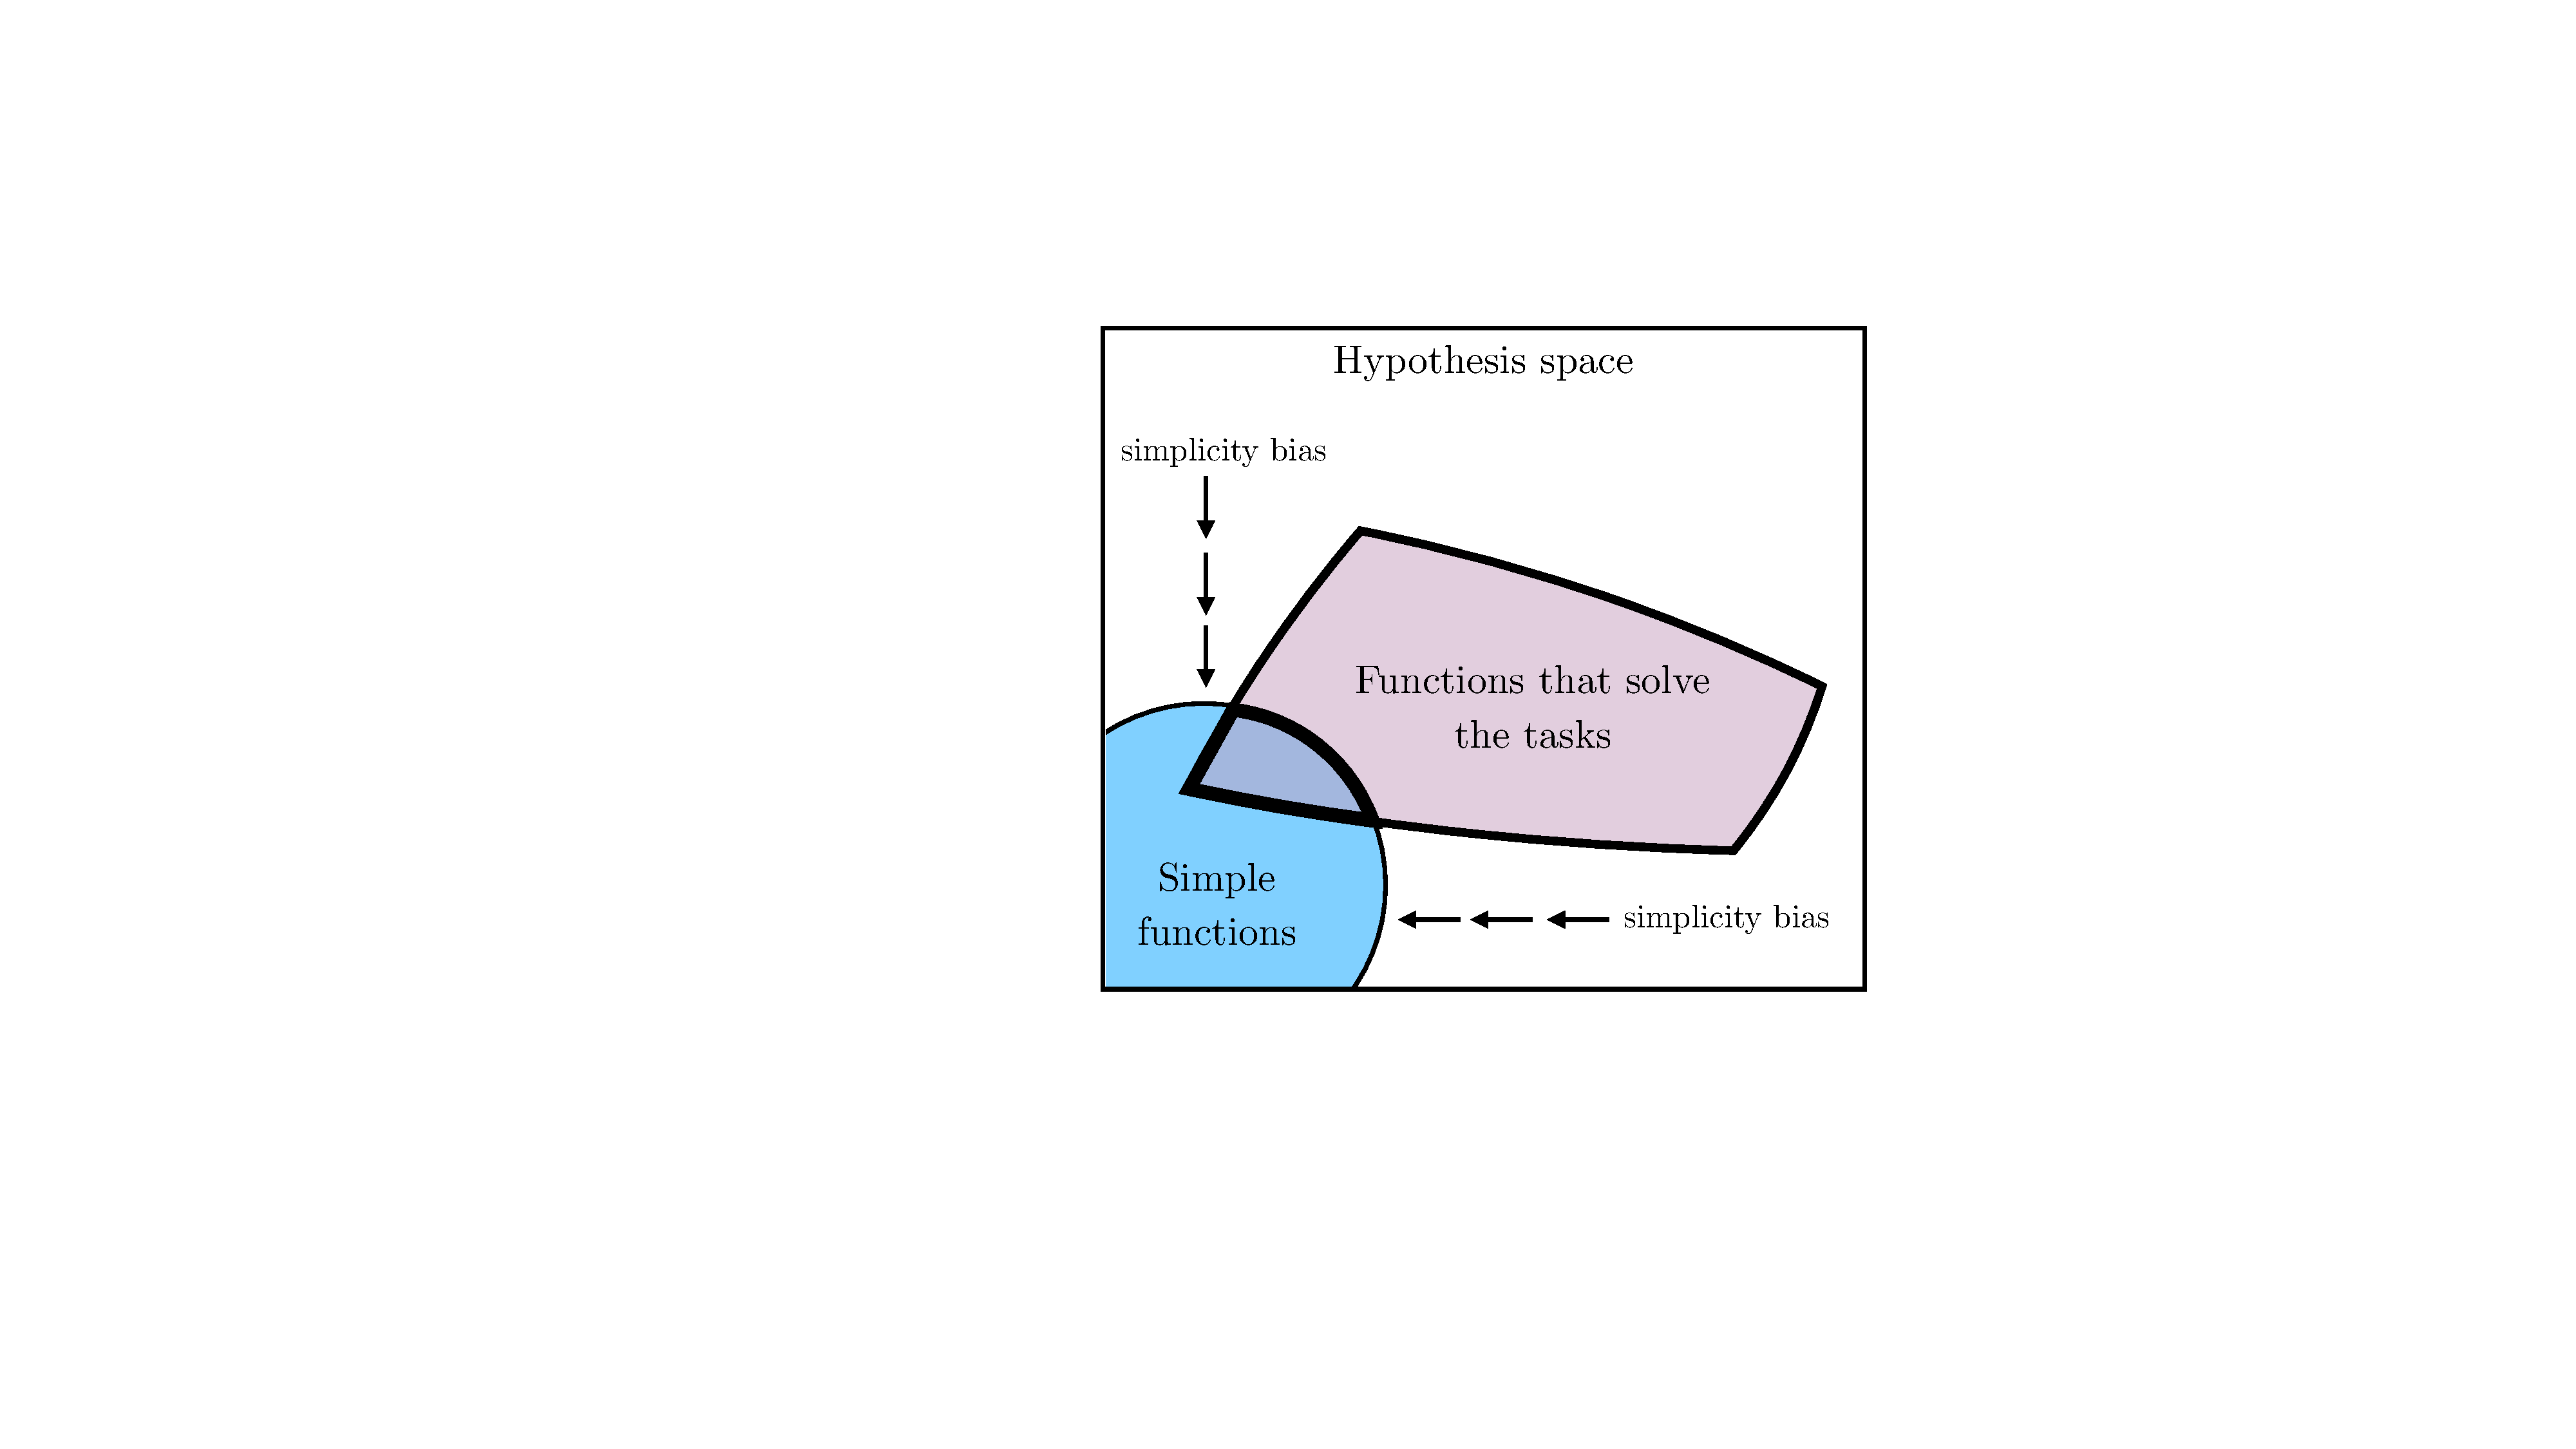
\includegraphics[width=0.825\linewidth]{figures/simplicity_hypothesis.pdf}\\[-7pt]
    \caption{\small \textbf{The Simplicity Bias Hypothesis:} Larger models have larger coverage of all possible ways to fit the same data. However, the implicit simplicity biases of deep networks encourage larger models to find the simplest of these solutions.}
    \label{fig:simplicity_hypothesis}
    \vspace{2pt}
\end{figure}
\section{What representation are we converging to?}\label{sec:what_rep}

% what is in the intersection of the multitask figure
% a good factorized world model 
% then kernels, bivariate, argument
% then say SSL related to that too

By now, we hope to have convinced the reader that task and data pressures, combined with increasing model capacity, can lead to convergence. We next turn our attention to \textit{what} exactly is the endpoint of all this convergence. 

Our central hypothesis, stated in~\Cref{fig:platonic_rep}, is that the representation we are converging toward is a statistical model of the underlying reality that generates our observations. Consistent with the multitask scaling hypothesis, such a representation would naturally be useful toward many tasks (or at least toward any task grounded in reality). Additionally, this representation might be relatively simple, assuming that scientists
% \jh{citation? could cite Murray GelMann} 
are correct in suggesting that the fundamental laws of nature are indeed simple functions \citep{gell1995quark}, in line with the simplicity bias hypothesis.

But what exactly do we mean by ``a statistical model of the underlying reality.'' In this section, we formalize one definition with concrete mathematical statements. \emph{Importantly}, this section should be read as just one concrete candidate for the form of the platonic representation; other candidates could be arrived at from other modeling assumptions. %Indeed, many prior theories have sought to define the optimal world representations for an intelligent agent; \eg, \citet{soatto2014visual} argue that the representation should capture minimal and sufficient statistics necessary to solve a set of tasks, \citet{richens2024robust} argue that agents must acquire a casual world model in order to be robust to distribution shifts, 

% We articulate our precise hypothesis as follows:
% \hypbox{The Cooccurrence Kernel Hypothesis}{%
% The platonic representation is characterized by the \textit{cooccurrence kernel}: this representation measures distance between observations as equal their pointwise mutual information, up to constant shift.}

% Figure \ref{XX} depicts the graphical model for our idealized world.

\subsection{An idealized world}
We consider a world that works as follows, consistent with the cartoon in \Cref{fig:platonic_rep}. The world consists of a sequence of $T$ discrete events, denoted as $\mathbf{Z} \triangleq [z_1, \ldots, z_T]$, sampled from some unknown distribution $\mathbb{P}(\mathbf{Z})$. Each event can be observed in various ways. An observation is a bijective, deterministic function $\texttt{obs}: \mathcal{Z} \rightarrow \cdot{}\,$ that maps events to an arbitrary measurement space, such as pixels, sounds, mass, force, torque, words, etc. 
Later, in \Cref{sec:limitations}, we discuss limitations and potential extensions to continuous and unbounded worlds, and stochastic observations, that could yield a model that better reflects real learning scenarios.

One can think of an event as corresponding to the state of the world at some point in time\footnote{Here we only analyze temporal sequences, but note that the same could be done with respect to events laid out in space instead.}, but it is also fine to simply consider an event as any variable that indexes observations, with no further physical meaning\footnote{This latter interpretation may be more consistent with Plato's intent. Scholars have argued that his allegory of the cave rejects any notion of a true world state~\cite{nettleship1897lecturesplato}. Instead, we could say that the joint distribution of observation indices is \textit{itself} the platonic reality.}. %The key property is that the same index $z$ maps to multiple datapoints, each a different measurement of the same underlying event.}.

In this idealized world, knowing $\mathbb{P}(\mathbf{Z})$ would be useful for many kinds of predictions; this would constitute a world model over the events that cause our observations~\citep{werbos1987learning,ha2018world,richens2024robust}. We will next show that a particular representation of $\mathbb{P}(\mathbf{Z})$ is recovered by certain contrastive learners.

\begin{figure*}[ht]
    % \vspace{10pt}
    \centering
    % 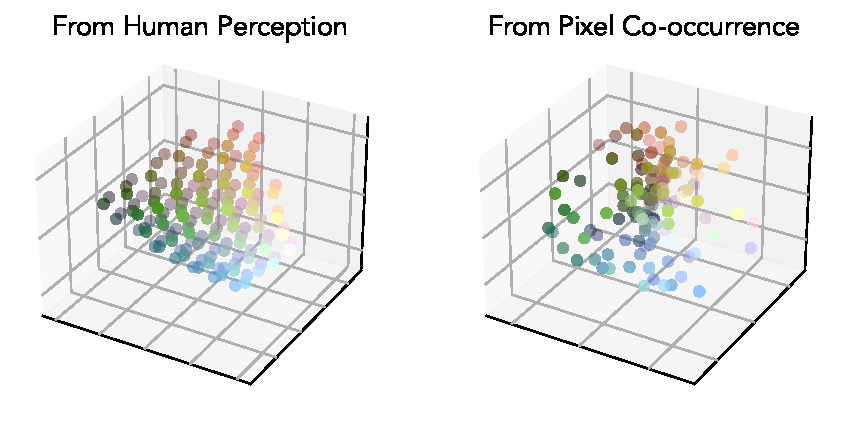
\includegraphics[width=0.495\linewidth]{figures/color_space.pdf}\hfill
    % 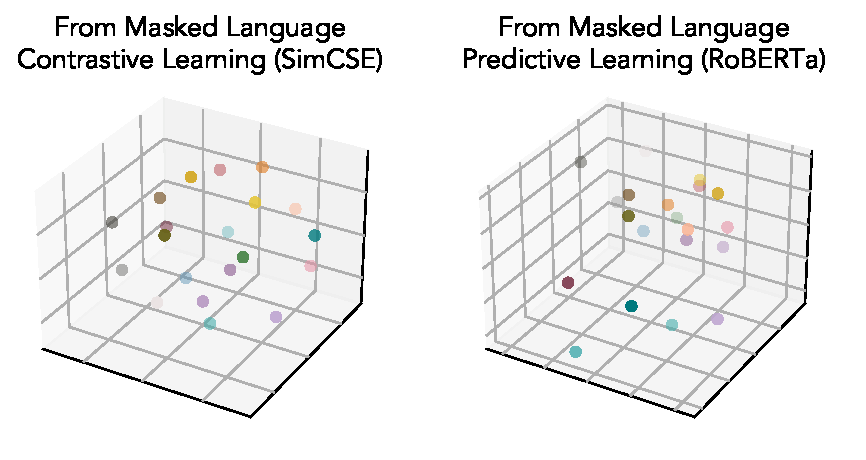
\includegraphics[width=0.495\linewidth]{figures/color_space_simcse_roberta.pdf}\\[-17pt]
    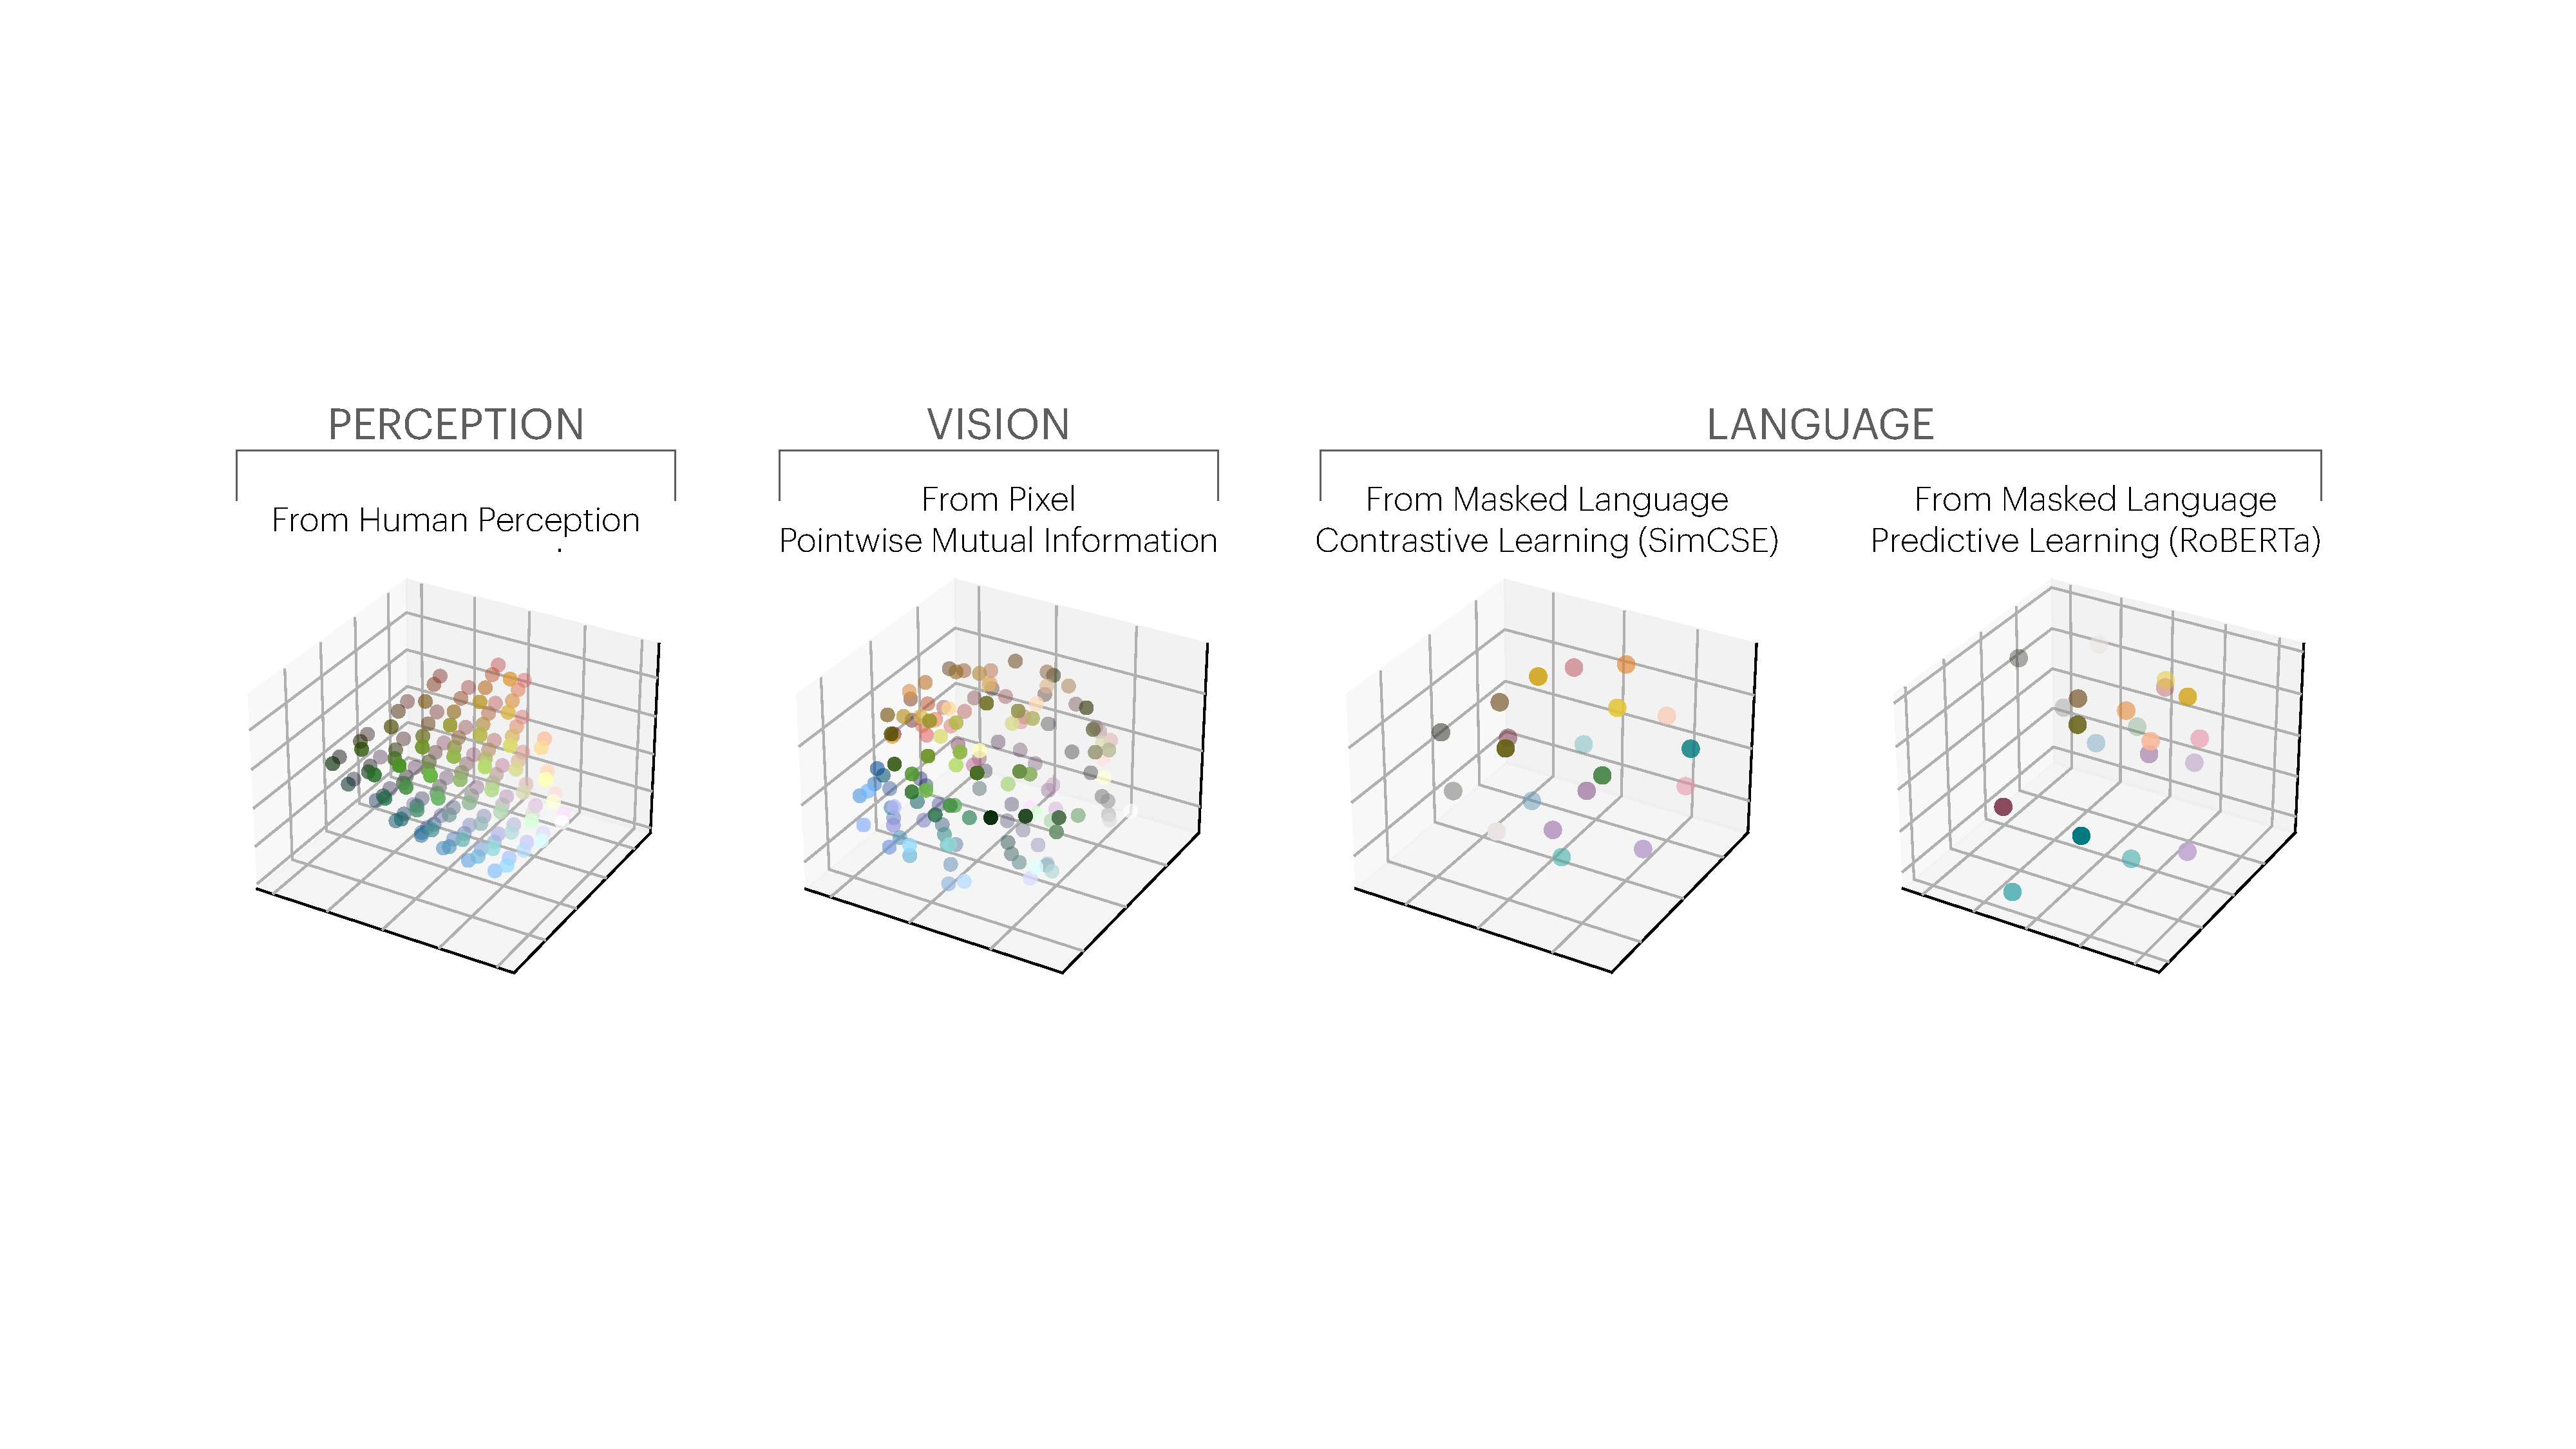
\includegraphics[width=0.99\linewidth,trim=174 352 188 295,clip]{figures/color_convergence.pdf}\\[-5pt]
    \caption{\small\textbf{Color cooccurrence in VISION and LANGUAGE yields perceptual organization:} Similar representations of color are obtained via, \textbf{from LEFT to RIGHT}, the perceptual layout from CIELAB color space,  cooccurrence in CIFAR-10 images, and language cooccurrence modeling (\citet{gao2021simcse,liu2019roberta}; computed roughly following \citet{abdou2021can}). Details in \Cref{sec:color_cooccurrences}.
    % We optimize 3-dimensional representations of colors based on cooccurrence in CIFAR-10 images (left), and obtain a similar layout with perceptual organization from CIELAB color space (right). \fixme{say something about language results on the right blah blah blah. } See Appendix \ref{sec:color_cooccurrences} for details.
    }
    \label{fig:color_pAB}
    % \vspace{10pt}
\end{figure*}

\subsection{A family of contrastive learners converge to a representation of $\mathbb{P}(\mathbf{Z})$}
\label{sec:simple-contra-kpmi}

Consider a contrastive learner that models observations that \textit{cooccur} together. For simplicity, we ground our discussion with the following definition of the \textit{cooccurrence probability}, $\Pco$, of two observations $x_a$ and $x_b$ both occurring within some  window $T_\mathsf{window}$: %leading to the \emph{symmetric} distribution:
\begin{align}
    \Pco(x_a, x_b) \hspace{0.1in} \propto \hspace{-0in} \sum_{(t, t') \colon \abs{t-t'} \leq T_\mathsf{window}} \hspace{-0.2in} \mathbb{P}(X_t = x_a, X_{t'} = x_b).\nonumber
\end{align}
Analogously, we can define $\Pco$ for $\mathbf{Z}$ and other observation modalities. Note that $\Pco$ is symmetric.

Consider \emph{positive pairs} as two observations nearby in time (sampled from $\Pco$) and \emph{negative pairs} as observations drawn from any point in time (sampled independently from the marginal). Our contrastive learner tries to classify if a pair is positive or negative by learning a representation $f_X \colon X \rightarrow \mathbb{R}^d$ such that the dot-product kernel approximates the log odds ratio up to some offset:
\begin{align}
    \langle f_X(x_a), f_X(x_b) \rangle 
    & \approx \log \frac{\mathbb{P}(\texttt{pos} \given x_a, x_b)}{\mathbb{P}(\texttt{neg} \given x_a, x_b)} + \tilde{c}_X(x_a) \\
    & = \log \frac{\Pco(x_a \given x_b)}{\Pco(x_a)} + c_X(x_a) \\
    & =  \Kpmi(x_a, x_b) + c_X(x_a), \label{eqn:contr-pmi}
\end{align}
where $\Kpmi$ is the pointwise mutual information (PMI) kernel, and $c_X(x_a)$ is constant in $x_b$. We note that this is a common setting for self-supervised contrastive learners with NCE objectives~\cite{gutmann2010noise,oord2018representation}, including SimCLR~\cite{chen2020simple} and SimCSE~\cite{gao2021simcse}.  (See \citet{oord2018representation} and \Cref{sec:analysis_contrastive-pmi} for detailed derivations.)

% So, positive pairs are sampled from $\Pco$ and negative pairs are sampled i.i.d. from its marginals.


% Positive pairs are two observations nearby in time and negative pairs are observations drawn from any point in time. Our learner tries to classify if a pair is positive or negative, i.e. it models $P(\texttt{pos} | x_a,x_b)$. It does so by learning a representation $f_{X}$ such that:
% \begin{align}
%     \langle f_X(x_a), f_{X}(x_b) \rangle \approx \log P(\texttt{pos} | x_a, x_b)
% \end{align}
% We note that is a common setting for self-supervised contrastive learners, such as DINO~\cite{caron2021emerging}, SimCSE~\cite{gao2021simcse}, etc.

% What representation does such a learner converge to? To get insight, define the \textit{cooccurrence probability}, $\Pco$, of two observations $x_a$ and $x_b$, as the probability of those observations both occurring within some temporal window. For simplicity, we will assume the window size is 1, so that
% \begin{align}
%     \Pco(x_a, x_b) \triangleq\frac{1}{2(T-1)}\sum_{t} ( & P(X_t = x_a, X_{t+1} = x_b) + {} \nonumber \\[-0.8ex]
%     & P(X_t = x_b, X_{t+1} = x_a)).
% \end{align}
% So, positive pairs are sampled from $\Pco$ and negative pairs are sampled i.i.d. from its marginals.

% %InfoNCE tries to classify whether a sample comes from the positive or negative distribution; 

% Intuitively, the optimal $\texttt{pos}$ vs $\texttt{neg}$ classifier should be related to the probability ratio between the positive and negative data distributions. Indeed it is, and it has the following form (as shown in \cite{CPC} and in Appendix XX):
% \begin{align}
%     P(\texttt{pos} | x_a,x_b) = \texttt{PMI}_{coor}(x_a,x_b) + C(x_a)
% \end{align}
% where $C(x_a)$ is a function constant in $x_b$ and $\texttt{PMI}$ is pointwise mutual information.

Under mild conditions that the world is smooth enough (see \Cref{sec:analysis_contrastive-exact-repr}), a choice of $f_X$ can exactly represent $\Kpmi$:
\begin{align}
    \langle f_X(x_a), f_X(x_b) \rangle &= \Kpmi(x_a,x_b) + c_X,
\end{align}
where we observed that $c_X(x_a)$ from \Cref{eqn:contr-pmi} must be a constant since both sides are symmetric.
% 
% Moreover, since $\mathbb{K}_{\texttt{PMI}}$ is a symmetric function, it must be that $C(x_a)$ is in fact a constant for all $x_a$. 

Therefore, the contrastive learners we consider are minimized by a representation $f_X$ whose kernel is $\Kpmi$ (up to a constant offset). With sufficient data and optimization, we will observe convergence to this point.

Thus we have convergence to a representation of the statistics of $X$, but what about $Z$? Recall that our idealized world consists of \textit{bijective} observation functions, which, over discrete random variables, preserve probabilities. So we have:
\begin{align*}
    \Pco(x_a, x_b) &= \Pco(z_a, z_b)\\
    \Kpmi(x_a, x_b) &= \Kpmi(z_a, z_b),
\end{align*}
% and likewise for other observation variables, 
where we use $\Pco$ and $\Kpmi$ in a modality-agnostic way to emphasize that different modalities share the same these quantities.
% This is due to the fact that bijective mappings over discrete random variables preserve probability~\cite{XX}. The same holds for $\texttt{PMI}$ rather than $\Pco$ (as $\textt{PMI}$ depends only on $\Pco$).
%from Eqn. \ref{eqn:coccurrence_model}, or from textbook probability theory~\cite{XX} (bijective mappings over discrete random variables preserve probability).

% Therefore, the \texttt{PMI} kernel for $X$ is equal to the \texttt{PMI} kernel for $Z$:
% \begin{align}
%     \mathbb{K}_{\texttt{PMI}}(x_a, x_b) = \mathbb{K}_{\texttt{PMI}}(z_a, z_b)
% \end{align}

%Now consider that we have another observation modality of the same set of events, $y = \texttt{obs}_Y(z)$. Our question is whether $f_Y$, trained on modality $Y$ will converge to the same kernel as $f_X$.

All these arguments hold not just for $X$ but also for $Y$ (or any other bijective, discrete modality), implying:
\begin{align}
    \Kpmi(z_a, z_b) 
    & = \langle f_X(x_a), f_X(x_b) \rangle - c_X \\
    & =     \langle f_Y(y_a), f_Y(y_b) \rangle  - c_Y.
\end{align}
Therefore, for any modality in our idealized world, we observe representational convergence to the same kernel, which represents certain pairwise statistics of $\mathbb{P}(\mathbf{Z})$.

This analysis suggests that certain representation learning algorithms may boil down to a simple rule: \textit{find an embedding in which similarity equals PMI}. We note that this idea is consistent with prior works that have used PMI as a similarity measure for clustering in vision and language (\eg, ~\citet{crisp_boundaries, isola_thesis, isola_cooc, chambers2008unsupervised}).

% We likewise define $\mathbb{P}_{\texttt{obs}}(x_a,x_b)$ as cooccurrence probability over observations in some modality $X$, where $x_a = \texttt{obs}_X(z_a)$ and $x_b=\texttt{obs}_X(z_b)$ are observations of cooccurring events $(z_a, z_b)\sim \mathbb{P}$.

% With these definitions:
% \begin{itemize}
%     \item Positive pairs are tuples of observations $(x, x^+) \sim \mathbb{P}
% _{\texttt{obs}}$
%     \item Negative pairs are tuples $x, x^- \iidsim P$
% \end{itemize}

% Now consider a learner that optimizes the InfoNCE objective over this data. 

% \begin{align}
%     \langle f_{\theta}(x_t), f_{\theta}(x_{t+1})) \rangle = \texttt{PMI}_{obs}(x_a,x_b)
% \end{align}



% Now consider a learner that optimizes InfoNCE objective over this data:
% \begin{align}
%     \argmin_{\theta} \underset{\substack{
%     x,x^+ \sim \mathbb{P}
% _{\texttt{obs}} \\
%     \{a^-_i\}_{i=1}^{M} \iidsim P
%     }}{\mathbb{E}} \Bigg[\log \frac{E_{\theta}(x,x^+)}{E_{\theta}(x,x^+) + \sum_i E_{\theta}(x,x_i^-)} \Bigg] \label{eqn:InfoNCE_obj}
% \end{align}

% The minimizer to this objective, as shown by XX, is:
% \begin{align}
%     E_{\theta}(x_a,x_b) = \log \frac{\mathbb{P}_{\texttt{obs}}(x_a,x_b)}{P(x_a)P(x_b)} + C(x_a) \\
%     \triangleq \texttt{PMI}_{obs}(x_a,x_b) + C(x_a)
% \end{align}
% where $C(x_a)$ is XX and $\texttt{PMI}$ is pointwise mutual information.

% Now, consider the following form for $E_{\theta}(x_a,x_b)$:
% \begin{align}
%     E_{\theta}(x_t,x_{t+1}) = \langle f_{\theta}(x_t), f_{\theta}(x_{t+1})) \rangle, \label{eqn:coccurrence_model}
% \end{align}

% Notice that any function $\texttt{PMI}$ can be represented in this way because $E_\theta$ can represent any positive semidefinite (PSD) kernel, and that $\log \mathbb{P}_\texttt{obs} + C$ is PSD for some $C$. \fixme{this is wrong} Therefore, the minimizer of \Cref{eqn:InfoNCE_obj} is a representation $f_\theta$ whose kernel is:
% \begin{align}
%     \langle f_{\theta}(x_t), f_{\theta}(x_{t+1})) \rangle = \texttt{PMI}_{obs}(x_a,x_b)
% \end{align}

% Therefore, the contrastive learner we have defined is minimized by representation $f_{\theta}$ whose kernel is $\texttt{PMI}$ (up to a constant offset); with sufficient data and optimization we will observe convergence to this point.


% \paragraph{Invariance to observation modality}
% Now consider that we have another observation modality of the same set of events, $y_t = \texttt{obs}_Y(z_t)$ and $y_{t+1} = \texttt{obs}_Y(z_{t+1})$. Our question is whether $f_Y$, trained on modality $Y$ will converge to the same kernel as $f_X$.

% Recall that our idealized world consists of \textit{bijective} observation functions over discrete random variables. In this setting, we have:
% \begin{align}
%     \mathbb{P}_{\texttt{obs}}(x_t, x_{t+1}) = \mathbb{P}(z_t, z_{t+1})
% \end{align}
% and likewise for other observation variables. This is due to the fact that bijective mappings over discrete random variables preserve probability~\cite{XX}.
% %from Eqn. \ref{eqn:coccurrence_model}, or from textbook probability theory~\cite{XX} (bijective mappings over discrete random variables preserve probability).

% Therefore, we can rewrite the cooccurrence kernel for some observation type $X$ in terms of pairwise probabilities over $Z$:
% \begin{align}
%     \mathbb{K}(x_t, x_{t+1}) = -\log \mathbb{P}_{\texttt{obs}}(z_t, z_{t+1})
% \end{align}
% All these arguments hold not just for $X$ but also for $Y$ (or any other bijective, discrete modality), implying:
% \begin{align}
%     \mathbb{K}(x_t, x_{t+1}) = \mathbb{K}(y_t, y_{t+1})
% \end{align}
% Therefore, we observe representational convergence to a common kernel across any two modalities in our idealized world.

% \subsection{The cooccurrence kernel}
% In this idealized world, knowing $P(\mathbf{Z})$ would be useful for many kinds of predictions; this would constitute a world model over the events that cause our observations~\cite{XX}. Our top level hypothesis is that the platonic representation is somehow a representation of $P(\mathbf{Z})$. We now provide a precise instantiation of this hypothesis.

% We have argued that a key property of representations is how they measure distance between inputs, i.e. their kernels. In this section we will only characterize representations up to their kernels (we leave open the question of whether order properties might matter too). The kernel is a pairwise function over inputs. If we are interested in representations of $z_1, \ldots, z_T$, then what matters is a pairwise function over $z$'s. A natural choice, then, is to look at pairwise probabilities.



% Presently, we are interested in representations of latent events $Z$. The kernel over $Z$ is a pairwise function over events.

% A representation of a latent events $Z$ 

% In the present analysis, we will restrict our attention to pairwise probabilities over events. We make this simplification because our characterization of representations is only up to their kernels, which are pairwise functions over inputs. In particular, we define the \textit{cooccurrence probability}, $\mathbb{P}$, of two events $z_a$ and $z_b$ as the probability of those events both occurring within some temporal window. For simplicity, we will assume the window size is 1, so that
% \begin{align}
%     \mathbb{P}(z_a, z_b) \triangleq\frac{1}{2(T-1)}\sum_{t} ( & P(Z_t = z_a, Z_{t+1} = z_b) + {} \nonumber \\[-0.8ex]
%     & P(Z_t = z_b, Z_{t+1} = z_a)).
% \end{align}

% From cooccurrence probability, we can define a kernel:
% \begin{align}
%     \mathbb{K}(z_t,z_{t+1}) \triangleq -\log \mathbb{P}(z_t,z_{t+1})
% \end{align}


% We will argue that the platonic representation is a model of cooccurrences of events. We leave open the question of whether representations might also be converging in terms of higher order statistics of $P(\mathbf{Z})$. 
% %We articulate our precise hypothesis as follows:
% %\hypbox{The Cooccurrence Kernel Hypothesis}{%
% %The platonic representation is characterized by the \textit{cooccurrence kernel}: this representation measures distance between observations as .}

% % Figure \ref{XX} depicts the graphical model for our idealized world.

% Define the \textit{cooccurrence kernel} $\mathbb{K}$ as
% \begin{align}
%     \mathbb{K}(x_t,x_{t+1}) \triangleq -\log \mathbb{P}_{\texttt{obs}}(x_t,x_{t+1})
% \end{align}



%\subsection{Does this analysis reflect real models?}
%\label{sec:ideal-world-limitations-extensions}

% connect analyses to pred and contr



\paragraph{A study in color}
We conduct a case study to verify that convergence does happen on real data.
% In particular, in the case of colors, 
\citet{abdou2021can} discovered that color distances in learned language representations, when trained to predict cooccurrences in \emph{text} \citep{devlin2018bert}, closely mirror human perception of these distances, which we reproduce in \Cref{fig:color_pAB} with both contrastive and predictive models. Interestingly, they noted an increasing similarity as models scale larger and become better at modeling \emph{text} cooccurrences. In \Cref{fig:color_pAB}, we also learn representations of color based on $\Kpmi$ from cooccurrences in \emph{images}. %, and arrive at the same perceptual organization. 
Indeed, learning cooccurrence statistics in either domain recovers roughly the \emph{same} perceptual representation. Details of this experiment are described in \Cref{sec:color_cooccurrences}. 

We believe that our simple model encapsulates essential aspects of complex real-world systems, and offers a path toward understanding the representation that models are converging to---a unified model that is proficient across various domains and modalities, grounded in the statistical properties of the underlying world. \Cref{sec:limitations} further elaborates some limitations.



%\paragraph{Demonstration: modeling color cooccurrences}


%\paragraph{\textcolor{red}{Demonstration: modeling language cooccurrences}}



\section{What are the implications of convergence?}\label{sec:implications}
% \jh{take a pass and clean up}

\paragraph{Scaling is sufficient, but not necessarily efficient} Our arguments are roughly in line with the claim that ``scale is all you need'' to reach high levels of intelligence. We have argued that as resources are scaled (\# parameters, \# datapoints, \# flops), representations are converging, regardless of other modeling choices and even data modality. %However, there is an x-axis to this convergence: we have cited and shown many cases where bigger, better performing models are more converged than smaller, worse performing models. %As datasets scale, models are trained on more tasks, bigger models are developed, and these models are trained longer with more compute, we expect that convergence will increase. 
Does this mean that scale is all that matters? Not quite: different methods can scale with different levels of \textit{efficiency} \citep{hestness2017deep,kaplan2020scaling}, and successful methods must still satisfy some general requirements (\eg, be a consistent estimator, model pairwise statistics of $\mathbb{P}(\mathbf{Z})$).
%\phil{maybe add some autoregressive thing here}

\paragraph{Training data can be shared across modalities} Suppose you have access to $N$ images and $M$ sentences, and want to learn the best representation. If there is indeed a modality-agnostic platonic representation, then \emph{both} image and language data should help find it.
% the image data should help find it, and so should the language data. 
The implication is that if you want to train the best vision model, you should train not just on  $N$ images but also on $M$ sentences. This is already becoming common practice~\cite{achiam2023gpt, radford2021learning}. Many vision models are finetuned from pre-trained LLMs. The other direction is less common, but also is implied by our hypothesis: if you want to build the best LLM, \textit{you should also train on image data}. Indeed, \citet{achiam2023gpt} showed that training on images improved performance on text. %claim evidence that this is true, where training on images improved performance on text. 
In theory, there should be some conversion ratio: a pixel is worth $a$ words for training LLMs, and a word is worth $b$ pixels for training vision models.

% \paragraph{Ease of conditional generation and model adaptation}
\paragraph{Ease of translation and adaptation across modalities}
When two representations are aligned, transitioning from one to the other should be a simple function that's easily obtained. Our hypothesis could explain the phenomenon that conditional generation is easier than unconditional~\citep{mirza2014conditional,liu2020selfconditioned,sauer2022styleganxl}, as the data we condition on may have the same platonic structure as the data we are generating. In line with this, recent work has found that representation-conditioning is even easier \citep{RCG2023}. Similarly, representational convergence could act as a bridge that lets us find mappings between domains even without paired data; this may underlie the success of unpaired translation in vision \citep{CycleGAN2017,shi2024diffusion,xie2022unsupervised} and language \citep{tranfeature2017tran,lample-etal-2018-phrase}. 
%if two representations share the same kernel (and it is sufficiently complex), then the mapping between the representations is uniquely defined~\citep{XX}. This property may explain the success of methods in unsupervised translation in vision \citep{CycleGAN2017,shi2024diffusion,xie2022unsupervised} and language \citep{tranfeature2017tran,lample-etal-2018-phrase}.  
%In practice, this property has enabled frequency analysis to solve substitution ciphers and underlies successes in unsupervised translation across vision \citep{CycleGAN2017,shi2024diffusion,xie2022unsupervised} and language \citep{tranfeature2017tran,lample-etal-2018-phrase}.
We emphasize that this doesn't mean that models trained on a single modality (\eg, language) can immediately process raw data from another (\eg, vision). What makes them adaptable to the new modalities is that they share a common modality-agnostic representation, and can readily process \emph{representations} of new modalities. 
Furthermore, this implies that language models would achieve some notion of grounding in the visual domain %\footnote{There are many definitions of grounding. Here we mean that visual concepts can be effectively encoded and decoded in the language model's representation space.}, 
even in the absence of cross-modal data\footnote{
In 1688, William Molyneux asked if a person born blind, upon gaining sight, could distinguish shapes by vision alone~\citep{locke_molyneaux}. Our arguments suggest they could not do so immediately, but after some visual experience, they could easily map shapes to their prior touch-based representations. Empirical data supports this, showing that congenitally blind children given sight can quickly learn these abilities~\citep{held2011newly}. 
}.
% 
% Regarding language Models, if they converge to the same representation as vision models, they achieve some notion of grounding\footnote{There are many definitions of grounding. Here we mean... \fixme{fixme}}, even in the absence of cross-modal data. 
The primary advantage of cross-modal data could then simply be sample efficiency. 
% Achieving a platonic representation is potentially more sample-efficient with cross-modal data than with unimodal data. 
%Moreover, representations may become the mainstream data transfer format because they are both more byte-efficient and easier for models to process.

% \jh{remove or combine with section below}
% \paragraph{Language models do not strictly need grounding} If LLMs converge to the same representation as vision models, then, in a certain sense, they become grounded\footnote{There are many definitions of grounding. Here we mean...} even without cross-modal data. What is then the advantage of cross-modal data. It could be efficiency. Arriving at the platonic representation may be more sample efficient with cross-modal data than with unimodal data [cites].

% \paragraph{Extending models to new modalities is easy} For two aligned representations, the mapping from one to the other should be a simple function that is easy to learn. However, this does not mean that models trained on one modality (\eg, language models) can be directly used to effectively process data from other modalities (\eg, visual content). Instead, they are easily adaptable to take in high-quality \emph{representations} of data from new modalities. 

% \paragraph{} Many machine learning pipelines require process data from multiple modalities, including learning mappings from one to another, or aggregating information from multiple sources. As representation spaces get better and more aligned, these spaces not only enable better task-solving, but also make it easier to learn such mappings/models that process representations from different modalities.

% \paragraph{Decreasing need for accessing raw data} 
% \jh{This section is confusing to me}
% As representations converge, the need for accessing raw data decreases, because training is as, if not more, efficient on a dataset of representations. Sharing the representation of a video clip is both more byte-efficient and easier for models to process. Aligned and high-quality representations enable multi-modal systems to better aggregate information from multiple modalities, and learn mappings among them. Datasets of representations may become more mainstream. 
% g
% \jh{scale will lead to convergence.}

% \subsection{A family of contrastive learners converge to a representation of $\mathbb{P}(\mathbf{Z})$}
% \label{sec:simple-contra-kpmi}

\paragraph{Scaling may reduce hallucination and bias} 
A prominent shortcoming of current LLMs is their propensity to hallucinate, or output false statements. If models are indeed converging toward an accurate model of reality, and scale powers this convergence, then we may expect hallucinations to decrease with scale. Of course, our hypothesis is conditioned on the training data for future models constituting a sufficiently lossless and diverse set of measurements. This may not come to pass, but it is an implication of our hypothesis worth pointing out. A similar argument can be made about certain kinds of bias. It has been shown that large models can exacerbate existing biases present in their training data~\citep{hall2022systematic}. Our hypothesis implies that, while this may be true, we should expect \textit{larger} models to amplify bias \textit{less}. This does not mean bias will be removed, rather that the model's biases will more accurately reflect the data's biases, rather than exacerbating them.

%As AI systems progress towards a more consistent interpretation of data, hallucinations present in the model can be reduced. These hallucinations are deviations the model makes from data -- distortions from unbalanced or limited representation of reality. While this by no means should deter existing research efforts in model safety, scaling up models to be more competent will allow for a more truthful depiction of reality. This also does not mean the biases that already exist in the model will be reduced; rather, it will be more truthfully reflected by the model.

% As AI systems progress towards a more consistent interpretation of data, the biases present in our data – distortions due to uneven or limited representation of reality – may be reduced. While this by no means should deter existing research efforts in model safety, scaling of models could potentially mitigate some of these biases, where competent models will have a more balanced and truthful depiction of reality.

% As AI systems evolve towards a more uniform understanding of data, biases inherent in our data can be distortions of reality due to uneven or limited coverage of projections of reality. As models scale, they have the potential to reduce these biases as they capture more diversity in data and cover a larger distribution of reality, moving closer to a more balanced and truthful depiction of reality.

% \paragraph{Limitations of LLMs, autoregressive models, etc} A common refrain in any era of AI is that the methods of the era are doomed to failure: children can't possibly learn grammars without strong priors due to the ``poverty of the stimulus''~\cite{chomsky1965aspects}; neural nets must not generalize because they have more parameters than data~\cite{zhang2016understanding}; autoregressive models cannot reason due to exponential compounding of errors during rollout~\cite{williams1989learning,lecun2022path}. History teaches us to be skeptical of these kinds of arguments, as very often, an approach that was once dismissed by mathematical argument ends up working out nonetheless. This doesn't mean the theory was necessarily wrong (although sometimes it is) but rather that the assumptions underlying those theories were off. %Now, like in past eras, we see similar critiques about how certain representation learning approaches must certainly fail~\cite{lecun2022path,YY,ZZ}. \fixme{not sure about this citation} 
% The evidence we have summarized and presented in this paper argues that representations are converging regardless of whether they are trained on vision data or language data, using a contrastive objective or a generative objective, and so forth. This does not mean that absolutely any algorithm will converge on the same representation, but rather that the class of learners that converge may be broader than has been previously thought, likely at different speeds.

\section{Counterexamples and limitations}\label{sec:limitations}

%We conclude by providing several counterexamples to our hypothesis and discuss limitations of its explanatory power.

\paragraph{Different modalities may contain different information}

One immediate objection to our hypothesis is: what about the information that is unique to a given modality? Can language really describe the ineffable experience of watching a total solar eclipse? Or, how could an image convey the a concept like ``I believe in the freedom of speech,'' which is easy to write in English? Two different models cannot converge to the same representation if they have access to fundamentally different information. 

More precisely, our mathematical argument in \Cref{sec:what_rep} only strictly holds for bijective projections of $\mathbf{Z}$, so that the information in all the projections is equivalent to the information in the underlying world. This will not hold true for either lossy or stochastic observation functions. Nonetheless, similar arguments have been made theoretically and empirically that cooccurrence relations are learned by practical contrastive \citep{tongzhouw2020hypersphere,zimmermann2021contrastive} and predictive learners \citep{papyan2020prevalence,roeder2021linear}.  
\citet{lu2021pretrained} and \citet{mirchandani2023large} also showed that models trained to autoregressively generate text also capture statistical relations in many other modalities, including symbolic reasoning, 
vision, protein folding, and robotics.

\begin{figure}[t!]
    \centering
    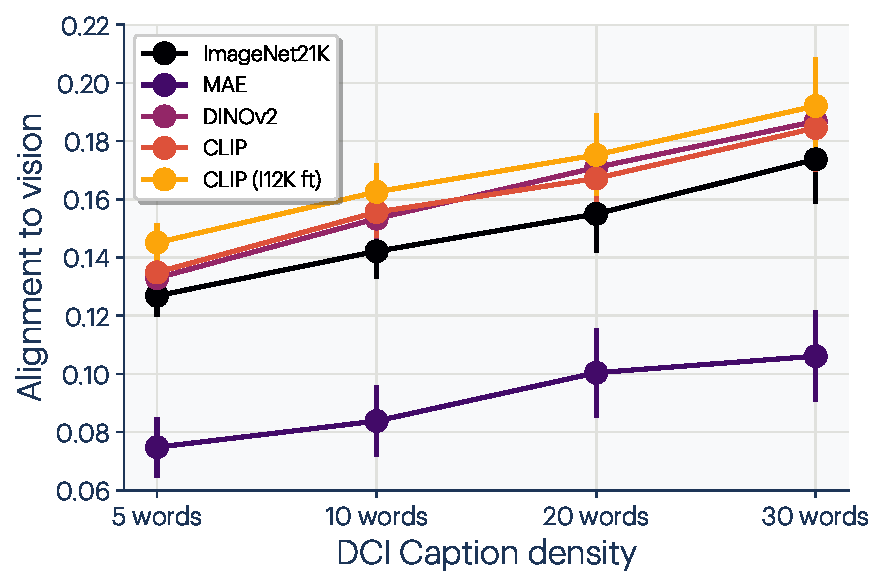
\includegraphics[width=\linewidth]{figures/caption_density_dci_combined.pdf}%
    \vspace{-11pt}%
    \caption{\small \textbf{Increasing caption density improves alignment:} We vary caption length using the Densely-Captioned-Images (DCI) dataset~\cite{urbanek2023picture}. Starting from a dense caption, we used LLaMA3-8B-Instruct~\cite{meta2024llama3} to summarize and generate coarse-grained captions. We compute the average alignment score across all vision and language models with standard deviation measured over the language models we evaluated. With denser captions, the mapping may become more bijective, leading to improved language-vision alignment scores.}
    \label{fig:caption_density}
\end{figure}

%But obviously a short caption is not fully informative about everything in an image. And an image is not as much information as a video. Clearly different projections contain different information. These facts stand in contrast to a strong form of our hypothesis: different representations \textit{can} capture different information, and thereby measure distances differently (lead to different kernels). 

A more nuanced version of our hypothesis will need to be developed to handle the case of non-bijective observations and abstract concepts. A starting point could be: different models will converge to the same representation \textit{when the input signals are sufficiently high information and the models are sufficiently high capacity}; when they are not, the lower-information representation will only align with the higher-information one up to a level capped by the mutual information between the input signals and by the capacity of each model. This cap might or might not be practically important. Popular representations like CLIP are explicitly optimized to only capture the shared information between vision and language, yet are highly successful on many pure vision tasks. 
%will be a ``blurred'' version of the higher information representation. 
We perform a preliminary test of the effect of information level in \Cref{fig:caption_density} (detailed in \Cref{sec:caption_density}), and find that the more descriptive (higher information) a caption is, the better its LLM representation aligns with the visual representation of the corresponding image.


%Is this idealized setting reflective of real learning problems, and what about learners that are not contrastive?



% Other learners work by predicting the next observation in a sequence given previous observations, aiming to model $P(x^2 | x^1)$ where $[x^1, x^2]$ is a training sequence. For these predictive learners, the cooccurrence probability, $P(x^1, x^2)$, is a sufficient statistic of the prediction problem, since $P(x^2 | x^1) = \frac{P(x^1, x^2)}{\int_{x^2} P(x^1, x^2) dx^2}$. Therefore, we conjecture that predictive objectives also lead to internal representations of cooccurrence probability\footnote{Note that $x^1$ and $x^2$ in predictive learning are \textit{not} iid, rather $x^2$ is an observation that occurs \textit{after} $x^1$}.

% In Appendix \ref{sec:analysis_contrastive_predictive}, we derive kernels for a few particular constrastive and predictive learners in idealized settings. The forms of these kernels are related to $K_{\texttt{coccur}}$ but not identical to it. Thus, our mathematical analysis does not precisely claim that all representations are converging to the \textit{exact} same thing, but it does suggest that they are converging to \textit{related} things. Our \textit{hypothesis} is that 1) these related representations are roughly the same in practical settings, 2) they are similar enough that we will observe continued convergence, even if the end points are slightly different, and 3) our idealized world is close enough to reality for these claims to hold in practice.

% %First we will argue that the platonic learner we have described is a kind of contrastive learner. Then we will argue that other popular learners are also benefitted from modeling $p_{\theta}(x^1,x^2)$, which suggests they may learn an internal model of the platonic kernel we have defined.


% % color
% % [todo] language cpation etc.

% \paragraph{Lossy projections}

% What if the observation function is not bijective? A class label is less information than a photo, so surely the representation of class label cannot match that of a photo.

% Yes, this is definitely a limitation of our hypothesis. The hypothesis requires refinement to match this setting.

\paragraph{Not all representations are presently converging}

Our argument has mainly focused on two modalities: vision and language. While we do expect other modalities will follow similar trends, we have yet to see the same level of convergence across all domains. For example, in robotics there is not yet a standardized approach to representing world states in the same way as there is for representing images and text. One limitation lies in the hardware used in robotics, which is often expensive and slow. This creates a bottleneck in the quantity and diversity of training data.

%In essence, in contrast to other AI domains, robotics is still in an early stage along the data axis. 

% For comparison, it might be insightful to understand why vision systems seem to have converged both computationally and biologically. In the majority of animals, vision has converged towards stereoscopic visual sensors, with the specific functionalities of these visual sensors tuned to suit their respective environmental niches, such as color perception and sensitivity to different light levels. This convergence is remarkable, considering the wide diversity in other aspects of bodily morphology among species. Even if there were better vision systems, due to the diminishing return (\textit{eg,} having an extra pair visual sensor), species have not adopted a better visual system. It is likely that morphology, just like vision, may have arrived at the point of diminishing return, but simply due to lower selective pressure, we observe large variability in what is considered a valid morphology. 
% (connection to the fact that this is why it is hard to standardize a robotic system)
% (The fact that there is universality implies stronger selective pressure)



%Imagine two scientists looking at the same result: a $\rho = 0.5$ correlation between neural measurements in the brain and in an artificial network. The former says, ``Wow, brains and machines are so similar! There correlation is about the same as the correlation between smoking and getting cancer.'' The latter replies, ``They are not at all alike. There correlation is just what you would get if you compared the reviews of Nicholas Cage movies per year to the number of shark attacks per year.'' Both statements are true. A middling correlation can be due to meaningful kinds of sameness or due to happenstance, or superficial covariates. 

%\bc{Isn't this why we do controls to check what a null hypothesis correlation baseline would be? (\eg, where p-value are shown)}

%\paragraph{A million synchronized brains} We have argued that a single neural net is similar to a single human. However, a population of neural nets is not necessarily like a population of humans. The neural nets can communicate with each other at much higher bandwidth. Humans mainly communicate just through speech and writing. Neural nets can send each other higher-dimensional internal representations, gradients, etc. Humans also are typically not all coordinated in their goals. Populations of AIs could be.


%\paragraph{Super-alignment and scale difference} Right now, the biggest models are of similar scale to a single human brain, in terms of numbers of neurons, connections, training data scale, etc (within a few orders of magnitude). It is likely that soon AIs will be far larger. This could push them farther out on the Anna Karenina axis. But it also could take them away from human-like intelligence, as humans may become relatively less converged. 

%AI systems can consume larger amount of data and achieve higher computational needs than humans. Moreover, AI systems have the differing selective pressure, hence, there may be a different convergence point, and even to as to diverge from humans.

% \paragraph{Quality-diversity}

% \paragraph{Perception is inference of truth}
% If all modalities are derived from truth, why are certain modalities converging slower. Is it simply the intrinsic cost associate to them?



\paragraph{Sociological bias in producing AI models}
Researcher bias and collective preferences within the AI community have shaped the trajectory of model development. %By favoring models that align closely with human intelligence, there may be an artificial sense of convergence toward human-like capabilities. 
There is often an explicit or implicit goal of designing AI systems that mimic human reasoning and performance, and this could lead to convergence toward human-like representations even if other kinds of intelligence are in fact possible. 
%and this may narrow the diversity of AI development paths. 
Additionally, the ``hardware lottery''~\cite{hooker2021hardware} suggests that the success of AI models can also depend on the compatibility of their design with available computational architectures, further contributing to convergent trends.

\paragraph{Special-purpose intelligences might not converge} 
Different intelligent systems can be designed to accomplish different tasks. For instance:
A bioinformatics systems might predict protein structure; 
%A voice assistant like Siri focuses on natural language understanding and providing user assistance.
an autonomous vehicle might follow lanes on highways. It's possible that not much is shared between these two narrow tasks. %Furthermore, the wheels of the vehicle itself being absent in biology is a testament to the divergent pressure from accomplishing the specific task of energy-efficient transport.
%An image recognition system is trained to identify objects or patterns in images.
Our argument only holds for intelligences that are optimized to perform well on \textit{many} tasks. We have argued that a representation of \textit{reality} is a structure that is useful across many tasks, but for any special purpose there may be shortcuts, or even effective representations detached from reality. Such shortcuts may be more efficient and necessary for continued improvements in specific domains. This will become more relevant if continued scaling comes up against boundary conditions around resources like energy and compute.

% \paragraph{Different design principles} 
% Human intelligence is the result of complex biological processes, including the structure and functioning of the human brain. AI systems, on the other hand, are designed using computational algorithms and models that are fundamentally different from biological processes. The underlying principles and mechanisms driving human intelligence and AI systems are distinct, which suggests that their outcomes and capabilities will also differ.


% We dive into each common representation learning algorithms and how it relates to co-occurecnces:


% \paragraph{Contrastive Learning and cooccurrence}
% Contrastive learning methods, which align similar or 'positive' pairs and differentiate from 'negative' pairs, are shown to optimize towards a function of Pointwise Mutual Information (PMI). In these methods, positive pairs are defined as co-occurring events, and negative pairs as random, independent events. The optimization of these methods leads to a kernel function that, although not perfectly, aligns closely with PMI of event pairs.

% \paragraph{Predictive Learning}
% Predictive learning models, which predict future events based on current context, are shown to optimize towards a kernel that measures the similarity in predictions about subsequent events. The analysis suggests that items are considered similar if they lead to similar predictions about the next event. This conceptually aligns with the idea that if two items predict similar outcomes for numerous events, they should be considered similar.

% \paragraph{Empirical Validation with Color Similarity}
% To empirically validate the theoretical findings, a simplified model based on color similarities is used. This model considers a world represented by sequences of state variables and observations in different modalities (such as images and text). It is shown that optimized models for different modalities (like vision and language) converge towards the same underlying distribution, effectively recovering the same color similarity function. This convergence suggests that as models are trained on more diverse and extensive data, they increasingly approximate the true distribution of the observed world.

% \paragraph{Limitations and Real-World Applicability}
% While the analysis is grounded in a simplified, discrete world with bijective observation functions, it is posited that these findings hold true in more complex, real-world scenarios. This implies that despite the inherent complexity and continuous nature of real-world data, optimized learning models are likely converging towards a universal representation of cooccurrences and event prediction.

% However, this idealized analysis has its limits, especially when considering the continuous nature of the real world and non-bijective observation functions. Despite these limitations, the model is believed to encapsulate essential aspects of more complex, real-world systems. This analysis offers a pathway towards understanding the essence of what representations converge to, supporting the hypothesis that learning systems are moving towards a unified model, proficient across various domains and modalities, fundamentally grounded in the cooccurrence of events.


%\paragraph{Plato's rebuttal} We have argued that the platonic representation is a direct reflection of physical reality. Plato, in contrast, distinguished between the physical world and some platonic ideal beyond it. ...\fixme{fix}


%\section{Limitations of measuring these trends}
\paragraph{
How do we measure alignment?
}
We focused on one particular alignment measure, mutual nearest-neighbor, in our experiments, and cited experiments using several others. However, there is active debate on the merits and deficiencies of all these ways of measuring alignment~\citep{bansal2021revisiting, sucholutsky2023getting}. We discuss our choice and show results for other alignment metrics in Appendix \ref{sec:align-metric}.

%Our work focuses on the search for alignment where we argue that the representations that are increasingly aligned among these intelligent systems. Without further investigation into the features that are unique to these systems, whether there is also increasing specialization unique to each intelligence is also occurring in addition to improved alignment over common features. This question can be answered with the exploration of alignment measures that require stricter notions of alignment. For instance, linear CKA requires alignment in the global geometry of representations between two systems whereas nearest neighbors is a local measure alignment.

% \paragraph{Why does language converge to vision and not vice versa?}
% For asymmetric measures of alignment, we find that vision models demonstrate increasing alignment to better language models but language models do not better align to stronger vision models. We posit this observation is due to the information content of visual information being higher than written language. In particular, a caption/class label of an image is a very coarse and lossy representation of the original image. We provide support for this hypothesis by showing the improved alignment (CKA scores) when we provide dense captions of images compared with only single-class labels.
% \bc{Reference CKA figure going from single-word label to dense caption. Also include WiT results since LLaVA created dense captions do have the confound of being generated by an LLM}

\paragraph{Lots left to explain} We have shown results where different models arrive at \textit{similar} but not the \textit{same} representations. For example, in \Cref{fig:alignment_comparisons}, alignment clearly increases but only reaches a score of $0.16$, according to our  mutual nearest-neighbor metric. The maximum theoretical value for this metric is $1$. Is a score of $0.16$ indicative of strong alignment with the remaining gap being ``noise'' or does it signify poor alignment with major differences left to explain? We leave this as an open question.%We question whether these trends will continue to eventually reach a score of 1. We suspect the trend will continue with an argument that 0.2 reflects a useful degree of alignment since language-vision models can be stitched together in practice with minimal adaptation. However, there is plenty of room for disagreement on these points.

% \section{Conclusion}

% Every new sample point is an observation that sheds light on the underlying mechanics of the world. Each additional piece of data inevitably shapes the trajectory of the model's hypothesis about the world. To put this in the parlance of deep learning, this evolving theory is the representation that the model learns from the data.
% While it's true that various representations may explain the same dataset, the volume of plausible hypotheses can only decrease as more data is observed. Ultimately, the representation with the highest predictive capacity that accommodates future observations outshines its counterparts.

% In homage to Newton-Smith's argument for convergent realism, it's important to note that the representation itself and the mechanistic process that led to these representations may undergo significant shifts over time. Yet, even in the face of such paradigm shifts and scientific revolutions, the representational power of these models is destined to improve. Indicating that despite the ebbs and flows of theoretical development, there remains constant progress toward better model representations.

% \begin{figure}
%     \centering
%     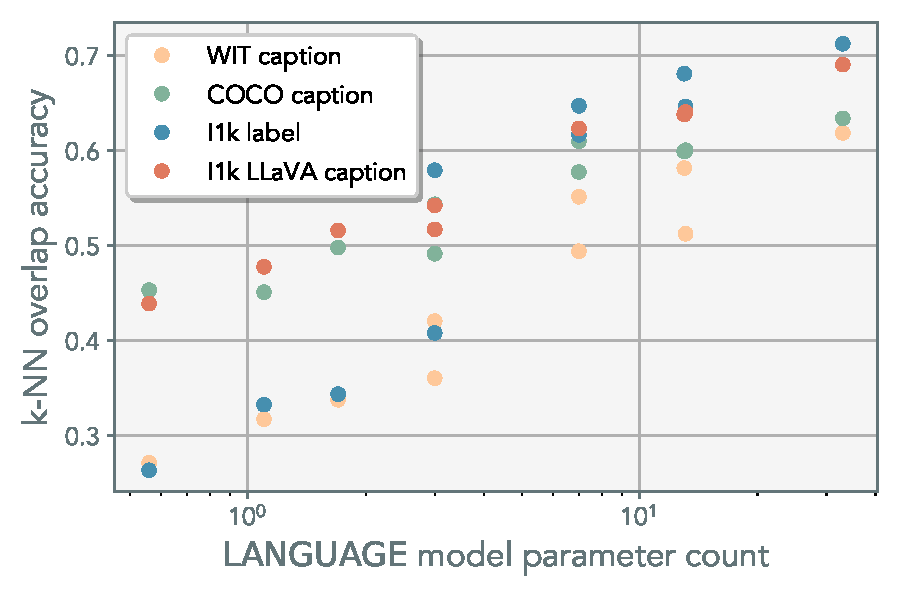
\includegraphics[width=1.\linewidth]{figures/llm_alignment.pdf}
%     \caption{(Rough-draft) Alignment of llm to llama65b. Right everything as alignment.}
%     \label{fig:}
% \end{figure}


% \begin{figure}
%     \centering
%     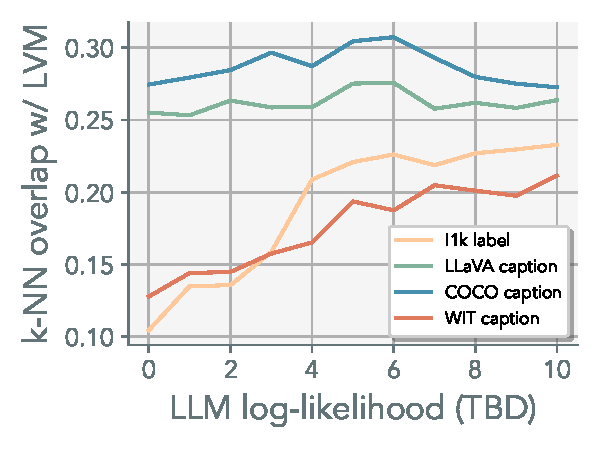
\includegraphics[width=0.75\linewidth]{figures/llm_dataset_overlap.pdf}
%     \caption{(Rough-draft) Alignment of LLM across datasets. *Some datasets don't improve with large LLMs. Investigate why simple LLMs are aligning.}
%     \label{fig:}
% \end{figure}

% \begin{figure}
%     \centering
%     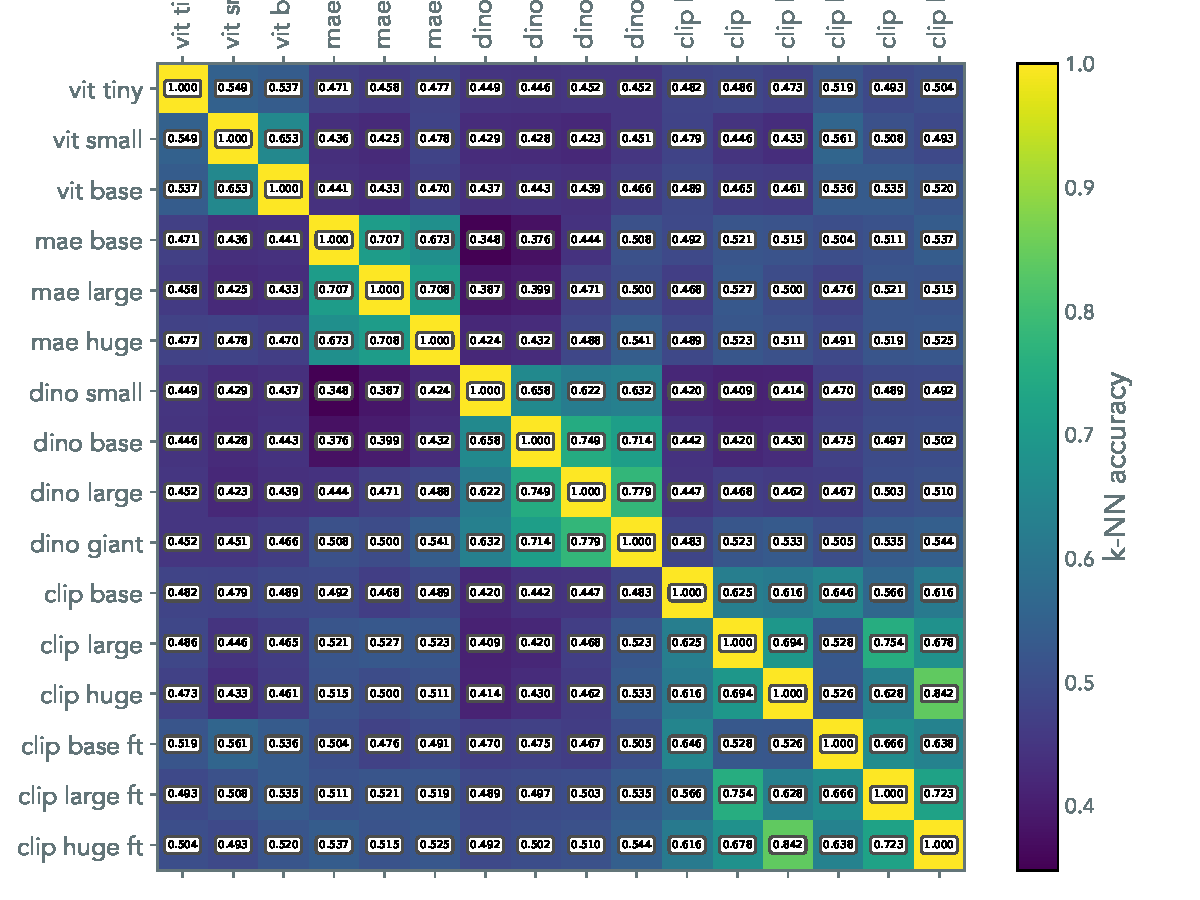
\includegraphics[width=1.\linewidth]{figures/lvm_wit_alignment_matrix.pdf}
%     \caption{(Rough-draft) Alignment of vision to vision}
%     \label{fig:}
% \end{figure}


% \begin{figure}
%     \centering
%     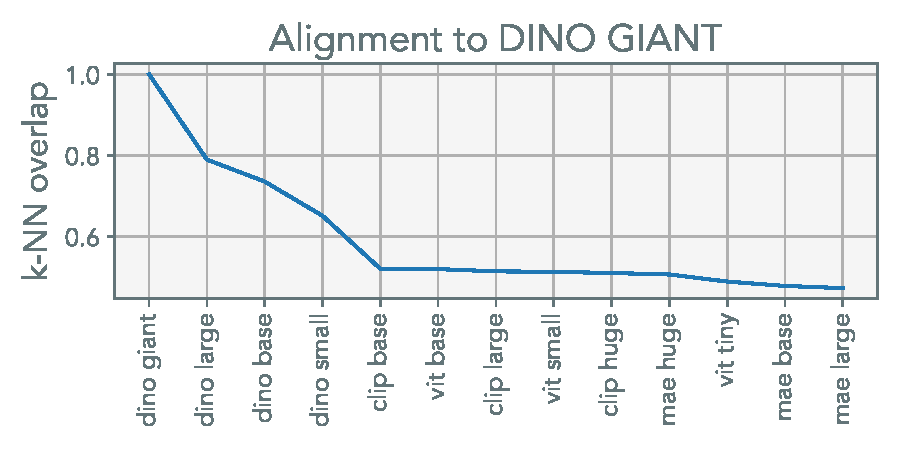
\includegraphics[width=0.75\linewidth]{figures/lvm_dino_giant_alignment.pdf}
%     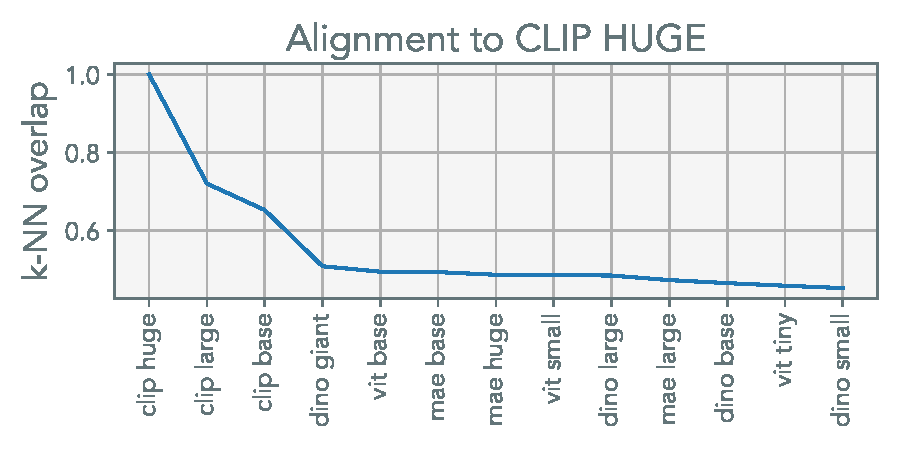
\includegraphics[width=0.75\linewidth]{figures/lvm_clip_huge_alignment.pdf}
%     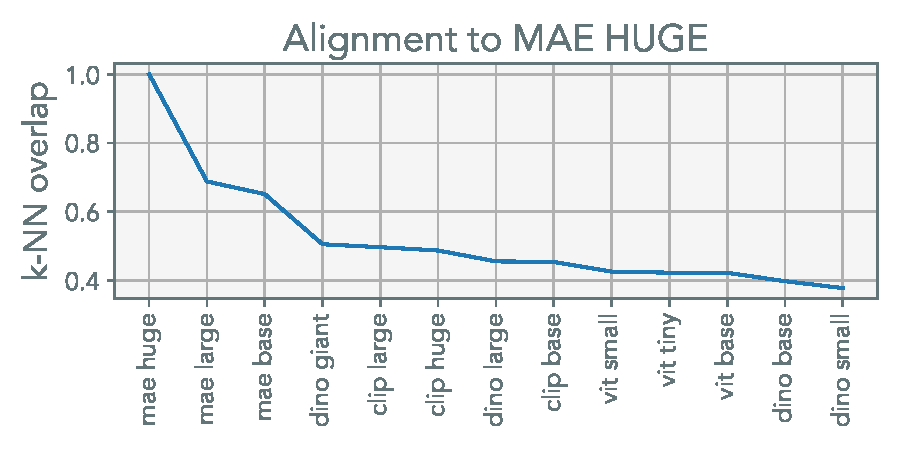
\includegraphics[width=0.75\linewidth]{figures/lvm_mae_huge_alignment.pdf}
%     \caption{(Rough-draft) Alignment of vision to vision}
%     \label{fig:}
% \end{figure}

% \section{Impact Statement}
% Our work has implications on the expectation of how AI will evolve in the future and our argument is that they will undergo a convergent process. If the convergent trend continues as we predict, it will have implications for the alignment of these models to human intelligence and beyond. This will impact the scope of methods to reduce the harmfulness of these systems as well as scope of vulnerabilities present among current systems.

\section*{Acknowledgements}

We thank \citeauthor{lindsey2014color} for sharing their data for our experiments shown in \Cref{fig:color_pAB}. We thank the anonymous reviewers for helpful feedback, and for providing the counterexample on how to visually convey ``I believe in the freedom of speech.'' Thanks for Yonglong Tian, Dilip Krishnan, Anna Decker, Yoon Kim, Jyo Pari, Ani Nrusimha, Dave Epstein, Victor Butoi, and Seungwook Han for helpful discussions and suggestions. We thank Mingzhong Sun for catching a typo. This work was supported by a Packard Fellowship and a Sloan Research Fellowship to P.I., by the MIT-IBM Watson AI Lab, by ONR MURI grant N00014-22-1-2740, by the Center for Brains, Minds, and Machines, the MIT Quest for Intelligence, NSF STC award CCF-1231216, the DARPA Knowledge Management at Scale and Speed (KMASS) program, and the DARPA Machine Common Sense (MCS) program.

% This paper presents work whose goal is to advance the field of Machine Learning. There are many potential societal consequences of our work, none which we feel must be specifically highlighted here.

% \section{To do}

% \jh{Todo: Anna Karenina -> Intelligence bottleneck, give full credit to Boaz Barak.}
% \jh{Add experiments: meta-plot in the alignment of methods to the human brain. Jim's work.}
% \jh{Add data from Dreamsim: larger models are closerly aligned with humans.}
% \jh{BAPPS, DREAMSIM, BRAINSCORE, THINGS}
% \jh{Alignment of models to models}
% \jh{MS-COCO brainscores like dataset?}
% \jh{Alignment of vision to LLMs: can we just annotate vision scores}
% \jh{Figure 1/2 illustrates there is 1 universal: Phillip}
% \jh{Figure 3: VISION (JACOB)}
% \jh{Figure 4: LLM (BRIAN)}
% \jh{FIgure 5: Generalization bounds.}
% \jh{UCE style for cross model convergence}
% \jh{to cite  and all read: https://www.biorxiv.org/content/10.1101/2022.03.28.485868v2.full.pdf}


{
\bibliographystyle{icml2024}
\bibliography{citations}
}
\clearpage

\newpage
\appendix
\onecolumn
% \section*{Appendix}
\appendix

% \section{Claimed Emergent Abilities}
% \label{app:claimed_emergent_abilities}

% We compile the models, tasks and metrics that different papers have claimed reveal emergent abilities of large language models. This list may be incomplete or inaccurate, but represents a good faith attempt to compile this information. Note: quantifying model scale when an ability emerges is complicated by the fact that different papers report model scale differently, either as (a) number of parameters \cite{brown2020language, ganguli2022predictability}, (b) effective number of parameters \cite{srivastava2022beyond} or (c) training FLOPs \cite{wei2022emergent}.

% \begin{table}[h!]
%     \centering
%     \begin{tabular}{|l|c|c|c|}
%     \hline
%         Task & Model Families & Metric & Model Scale at Emergence \\
%         \hline
%         2-Digit Addition \cite{brown2020language} & GPT-3 & Accuracy & 13B Parameters\\
%         2-Digit Subtraction \cite{brown2020language} & GPT-3 & Accuracy & 13B Parameters\\
%         3-Digit Addition \cite{brown2020language, ganguli2022predictability} & GPT-3 & Accuracy & 175B Parameters\\
%         3-Digit Subtraction \cite{brown2020language} & GPT-3 & Accuracy & 175B Parameters\\
%         MMLU \cite{ganguli2022predictability} & GPT-3, Gopher & Accuracy & 200B, 300B Parameters\\
%         Program Synthesis \cite{ganguli2022predictability} & Google Internal & \% Samples Solving Task & 200B Parameters\\
%         Figure of Speech Detection \cite{srivastava2022beyond} & ? & ? & $\sim 10^{11}$ Effective Parameters \\
%         IPA Transliterate \cite{srivastava2022beyond, wei2022emergent} & LaMDA, GPT-3 & BLEU & $\sim 10^{23}, \sim 10^{23}$ Training FLOPs\\
%         Periodic Elements \cite{srivastava2022beyond} & ? & ? & ?\\
%         Modified Arithmetic \cite{srivastava2022beyond, wei2022emergent} & GPT-3, LaMDA & Accuracy & $\sim 10^{23}, \sim 10^{24}$ Training FLOPs\\
%         Repeat Copy Logic \cite{srivastava2022beyond} & ? & ? & $10^{11}$ Effective Parameters\\
%         Word Unscrambling \cite{srivastava2022beyond, wei2022emergent} & LaMDA & Exact Match & $\sim 10^{24}$ Training FLOPs\\
%         Persian QA \cite{wei2022emergent} & PaLM & Exact Match & $\sim 10^{24}$ Training FLOPs\\
%         Truthful QA \cite{wei2022emergent} & Gopher & Accuracy & $\sim 10^{23}$ Training FLOPs\\
%         Grounded Mappings \cite{wei2022emergent} & ? & ? & ?\\
%         Multi-task NLU \cite{wei2022emergent} & ? & ? & ?\\
%         Word in context \cite{wei2022emergent} & ? & ? & $\sim 10^{24}$ Training FLOPs\\
%         \hline
%     \end{tabular}
%     \newline
%     \caption{\textbf{Tasks, model families, metrics and number of parameters for emergent abilities.}}
%     \label{tab:my_label}
% \end{table}


% \section{Exponentiated Negative Cross Entropy Lower Bounds Accuracy}
% \label{app:acc_bound}

% Consider batch size $B$ with length $L$. During training i.e. with teacher-forcing, the per-token accuracy (averaged over batch index $b$ and sequence index $l$) is defined as:
% %
% \begin{align}
%     \text{Acc} &\defeq \frac{1}{B} \sum_b \frac{1}{L} \sum_l p(t_{bl}^* | t_{b, <l}^*)\\
%     &= \frac{1}{BL} \sum_{b, l} p(t_{bl}^* | t_{b, <l}^*)
% \end{align}

% The cross entropy (commonly averaged over the batch) is defined as:
% %
% \begin{align}
%     \mathcal{L}_{CE} &\defeq -\frac{1}{B} \sum_b \log p(t_{b 1}^*, ..., t_{b L}^*)\\
%     &= -\frac{1}{B} \sum_b \log \prod_l p(t_{b l}^*| t_{b, <l}^*)\\
%     &= -\frac{1}{B} \sum_{b, l} \log p(t_{bl}^* | t_{b, <l}^*)
% \end{align}

% To make the comparison between accuracy and cross entropy a little easier, let's normalize the cross entropy by the sequence length:
% %
% \begin{align}
%     \mathcal{L}_{CE/L} &\defeq \frac{1}{L}\mathcal{L}_{CE}\\
%     &=  -\frac{1}{BL} \sum_{b, l} \log p(t_{bl}^* | t_{b, <l}^*)
% \end{align}

% Recall that Jensen's inequality tells us that for any random variable $X$, $\log \mathbb{E}[X] \geq \mathbb{E}[\log X]$. The relationship between sequence-length-normalized cross entropy and accuracy is thus:
% %
% \begin{align}
%     -\mathcal{L}_{CE/L} = \frac{1}{BL} \sum_{b, l} \log p(t_{bl}^* | t_{b <l}^*) &\leq \log \frac{1}{BL} \sum_{b, l}  p(t_{bl}^* | t_{b <l}^*) = \log \text{Acc}\\
%     \exp(- \mathcal{L}_{CE/L}) &\leq \text{Acc}
% \end{align}

% Consequently, we see that driving the cross entropy loss to $0$ necessarily drives the accuracy to $1$.

% TODO: Can we use the second moment method to derive bounds on how (un)likely a subset of tokens are to deviate from the mean?


\section{Approximate Behavior of Metrics on Sequential Data}
\label{app:metric_scaling}

How do different metrics behave when used to measure autoregressive model outputs? Precisely answering this question is tricky and possibly analytically unsolvable, so we provide an approximate answer here.

Notationally, we consider $N$ test data of length $L$ (here, length is measured in tokens) with targets denoted $t_n \defeq (t_{n1}, t_{n2}, ... t_{nL})$, the autoregressive model has a true-but-unknown per-token error probability of $\epsilon \in [0, 1]$ and the model outputs prediction $\hat{t}_n \defeq (\hat{t}_{n1}, \hat{t}_{n2}, ... \hat{t}_{nL})$. This assumes that the model's per-token error probability is constant, which is empirically false, but modeling the complex dependencies of errors is beyond our scope.

\subsection{Per-Token Error Probability is Resolution-Limited}
\label{app:metric_scaling:resolution_limited}

Note that because we have $N$ test data, each of length $L$, our resolution for viewing the per-token error probability $\epsilon$ is limited by $1/NL$. 
Here, resolution refers to ``the smallest interval measurable by a scientific instrument; the resolving power."
To explain what resolution means via an example, suppose one wants to measure a coin's probability of yielding heads.
After a single coin flip, only two outcomes are possible (H, T), so the resolution-limited probability of heads is either $0$ or $1$.
After two coin flips, four outcomes are possible (HH, HT, TH, TT), so the resolution-limited probability of heads is now one of $0, 0.5, 1$.
After $F$ coin flips, we can only resolve the coin's probability of yielding heads up to $1/F$.
Consequently, we introduce a resolution-limited notation:
%
\begin{equation}
    \nint{a}_b \defeq \text{$a$ rounded to the nearest integer multiple of $1/b$}
\end{equation}

\subsection{Token Edit Distance}
\label{app:metric_scaling:token_edit_distance}

We first consider an adaptation of the Levenshtein (string edit) distance for models that function on tokens rather than characters, an adaptation we term the \textit{token edit distance}. The token edit distance between two token sequences $t_n, \hat{t_n}$ is defined as the integer number of additions, deletions or substitutions necessary to transform $t_n$ into $\hat{t}_n$ (or vice versa).

\begin{align}
    \text{Token Edit Distance}(t_n, \hat{t}_n)  &\defeq \text{Num Substitutions} + \text{Num. Additions} + \text{Num. Deletions}\\
    &= \sum_{\ell =1}^L \mathbb{I}[t_{n\ell} \neq \hat{t}_{n\ell}] + \text{Num. Additions} + \text{Num. Deletions}\\
    &\geq \sum_{\ell =1}^L \mathbb{I}[t_{n\ell} \neq \hat{t}_{n\ell}]
\end{align}

The expected token edit distance is therefore:

\begin{align}
    \mathbb{E}[\text{Token Edit Distance}(t_n, \hat{t}_n)] &\geq \mathbb{E}[\sum_{\ell =1}^L \mathbb{I}[t_{n\ell} \neq \hat{t}_{n\ell}]]\\
    &= \sum_{\ell =1}^L p(t_{n\ell} \neq \hat{t}_{n\ell})\\
    &\approx L (1 - \epsilon)
\end{align}

The resolution-limited expected token edit distance is therefore:

\begin{equation}
    \nint{\mathbb{E}[\text{Token Edit Distance}(t_n, \hat{t}_n)]}_{NL} \geq L \Big(1 - \nint{\epsilon}_{NL} \Big)
\end{equation}

From this, we see that the expected token edit distance scales approximately linearly with the resolution-limited per-token probability. The real rate is slightly higher than linear because additions and deletions contribute an additional non-negative cost, but modeling this requires a model of how likely the model is to overproduce or underproduce tokens, which is something we do not currently possess.

\subsection{Accuracy}
\label{app:metric_scaling:accuracy}

\begin{align}
    \text{Accuracy}(t_n, \hat{t}_n) &\defeq \mathbb{I}[\text{No additions}] \, \mathbb{I}[\text{No deletions}] \, \prod_{l=1}^L \mathbb{I}[t_{nl} = \hat{t}_{nl}]\\
    &\approx \prod_{l=1}^L \mathbb{I}[t_{nl} = \hat{t}_{nl}]
\end{align}

As with the Token Edit Distance (App. \ref{app:metric_scaling:accuracy}), we ignore how likely the language model is to overproduce or underproduce tokens because we do not have a good model of this process. Continuing along,

\begin{align}
    \mathbb{E}[\log \text{Accuracy}] &= \sum_l \mathbb{E}[\log \mathbb{I}[t_{nl} = \hat{t}_{nl}]]\\
    &\leq \sum_l \log \mathbb{E}[\mathbb{I}[t_{nl} = \hat{t}_{nl}]]\\
    &\approx L \log (1- \epsilon)
    % \exp(\mathbb{E}[\log \text{Accuracy}]) &= \exp (\sum_l \mathbb{E}[\log \mathbb{I}(t_{nl}, \hat{t}_{nl})])\\
    % &=
\end{align}

Taking an approximation that would make most mathematicians cry:

\begin{align}
    \mathbb{E}[\text{Accuracy}] &\approx \exp(\mathbb{E}[\log \text{Accuracy}])\\
    &= (1 - \epsilon)^L\\
\end{align}

This reveals that accuracy \textbf{approximately} falls geometrically with target token length. The resolution-limited expected accuracy is therefore:

\begin{equation}
    \nint{\mathbb{E}[\text{Accuracy}]}_{NL} = \nint{(1 - \epsilon)^L}_{NL}
\end{equation}

From this we can see that choosing a nonlinear metric like Accuracy is affected significantly more by limited resolution because Accuracy forces one to distinguish quantities that decay rapidly.

\subsection{ROUGE-L-Sum}
\label{app:metric_scaling:rougeLsum}

\begin{figure}
    \centering
    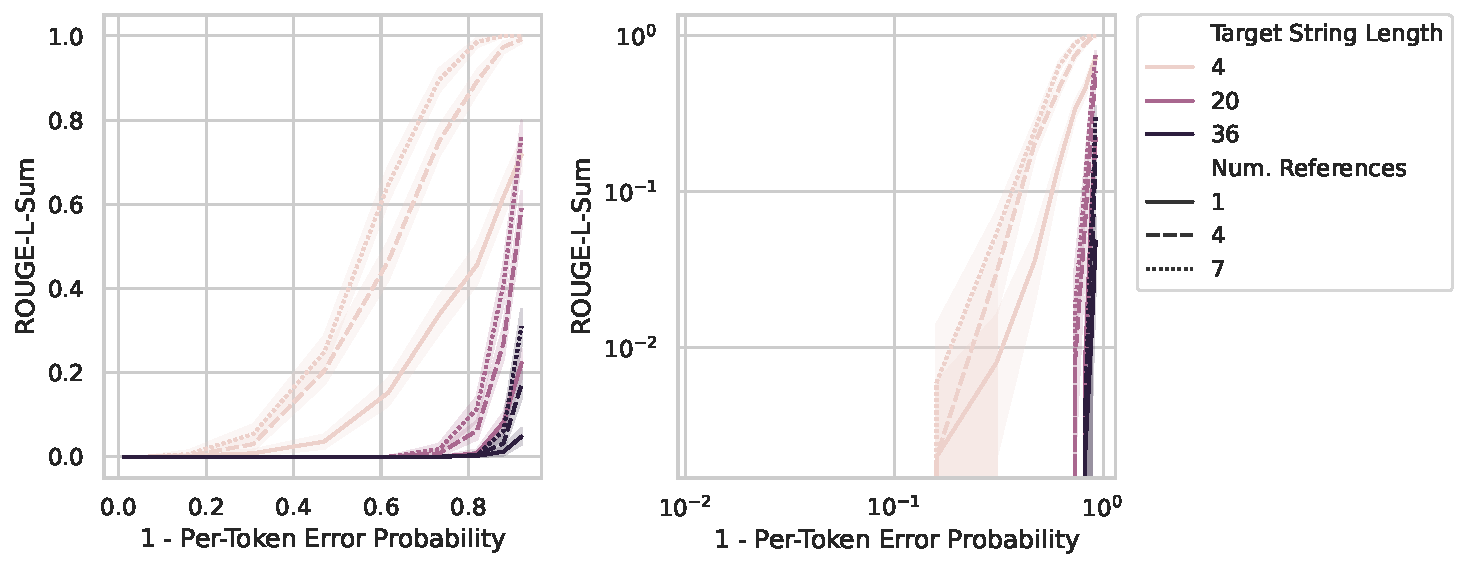
\includegraphics[width=0.95\textwidth]{figures/rouge_understanding/rougeLsum_vs_token_error_prob_scaling_simulation.pdf}
    \caption{\textbf{ROUGE-L-Sum is a sharp metric.} Simulations show that as the per-token error probability slightly increase (e.g. from 0.05 to 0.1), the ROUGE-L-Sum metric sharply falls.}
    \label{fig:app:metric_scaling:rougeLsum}
\end{figure}


Another BIG-Bench metric \cite{srivastava2022beyond} is ROUGE-L-Sum \cite{lin2004rouge}, a metric based on the longest common subsequence (LCS) between two sequences. Section 3.2 of \cite{lin2004rouge} gives the exact definition, but the key property is that ROUGE-L-Sum measures the ``union" LCS, which means ``stitching" together LCSs across the candidate and multiple references. As explained in the original paper: if the candidate sequence is $c = w_1 w_2 w_3 w_4 w_5$, and if there are two reference sequences $r_1 = w_1 w_2 w_6 w_7 w_8$ and $r_2 = w_1 w_3 w_8 w_9 w_5$, then $LCS(r_1, c) = w_1 w_2$ and $LCS(r_2, c) =w_1 w_3 w_5$, then the \textit{union} 
-LCS of $c, r_1, r_2$ is $w_1 w_2 w_3 w_5$, with length 4. Intuitively, this disproportionately benefits models with smaller error rates because their mistakes can be ``stitched" across multiple references; this is confirmed in simulation (Fig. \ref{fig:app:metric_scaling:rougeLsum}).


% \subsection{BLEU}
% \label{app:metric_scaling:bleu}


% \subsection{Emergence does not require on scaling laws: decreasing cross-entropy loss and stricter exact match is all you need }

% The goal of this section is to show that scaling laws are not necessary to create emergence and that many functional forms of the loss are valid as long as the form decreases as some other variable decreases -- say the number of parameters in the model.
% This typically holds in modern machine learning. 
% We do this by considering different functional forms of the cross entropy $CE(N)$, as a function of the number of parameters $N$, and show emergence, i.e. sharpness and unpredictability.
% We illustrate this by showing the programmer can exaggerate the sharpness (and therefore emergence) by implying increasing the exact number of tokens required to get correct in the accuracy, i.e. increasing $L$ in our notation.

% \subsubsection{Argument}

% Recall from section \ref{sec:alt_explanation} the accuracy requiring all $L$ tokens to be correct for a model of size $N$ as a function of cross-entropy $CE(N)$:

% \begin{equation*}
%     \text{Accuracy}(N) \approx p_N(\text{single token correct})^{\text{num. of tokens}} = \exp \Big(- CE(N) \Big)^L
% \end{equation*}

% We plot this equation using three functional forms for a decreasing cross-entropy loss in figure \ref{fig:decreasing_loss_leads_to_emergence_as_L_increases} for increasing values of $L$.
% These increasing values of $L$ induce a sharper -- therefore, seemingly more emergent curve when plotting the accuracy. 
% This means that if the programmer simply requires a stricter accuracy, he can make a perfectly smooth and predictable cross-entropy loss suddenly become sharp and unpredictable, i.e. ``emergent". 
% We show numerically it is independent of the functional form and instead that it only requires the cross-entropy to be decreasing and the accuracy metric to have some non-linear transformation that makes it sharper. 
% Therefore, if one had only tracked the cross-entropy loss instead, one could have had a smooth predictable curve for the models.
% This implies small-scale experimentation is still relevant, and we wish to highly that GPT-4 \cite{gpt4} small-scale experiment in conjunction with scaling loss. 
% We'd like to emphasize that changing the evaluation metric can suddenly induce emergence, and it is not an intrinsic property of the model. 

% %The goal will be to show that if $CE(N)$ decreases with different functional forms that $acc$ is emergent (either sharp or unpredictable).
% % TODO: sharp due to L
% % TODO: unpredictable due to constant and L

% \begin{figure}[htbp]
%   \centering
%   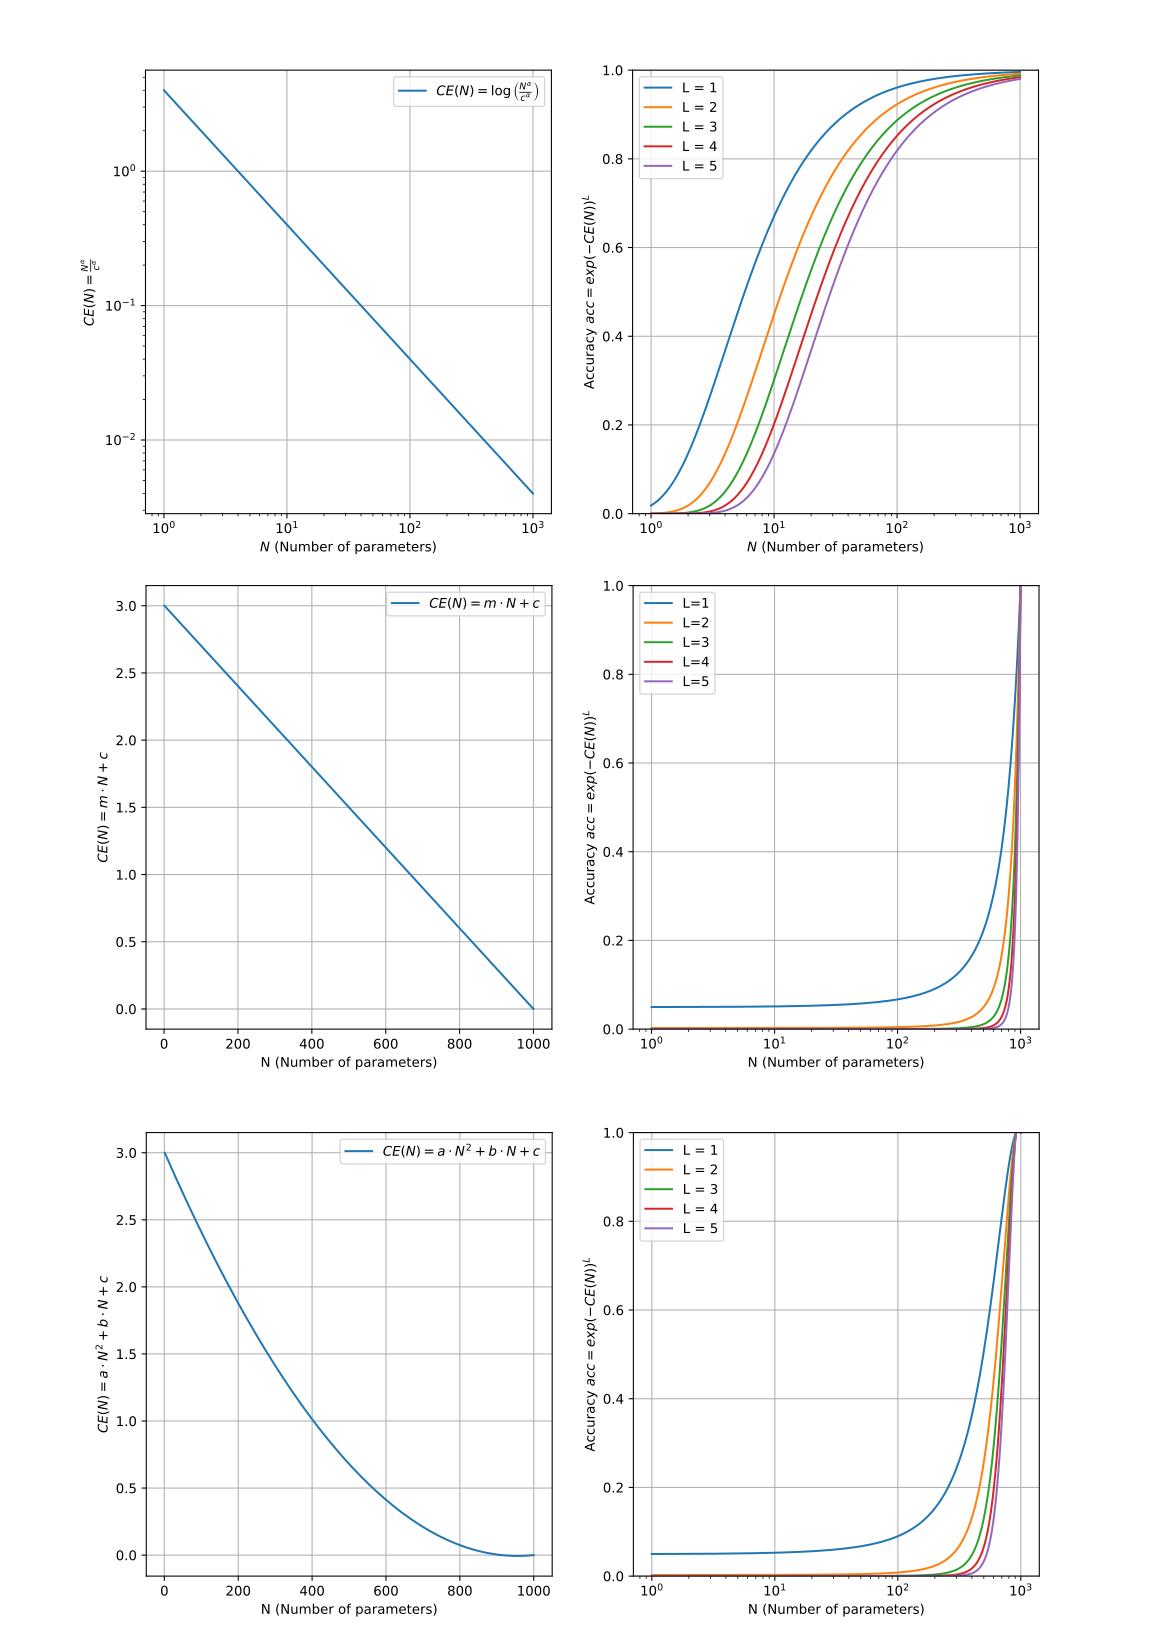
\includegraphics[width=0.8\textwidth]{figures/loss_decreasing_leads_to_emergence/decreasing_loss_leads_to_emergence_as_L_increases.png}
%   \caption{
%   \textbf{Emergence does not depend on scaling laws: any decreasing cross-entropy loss induces apparent emergence as L increases as you require more tokens to be exactly correct, i.e. L increases.}
%   The first row shows the same argument as in the main section, where a decreasing cross-entropy loss as a scaling law induces emergence as $L$ increases.
%   The second row shows the that apparent emergence is induced even when the cross-entropy loss decreases linearly.
%   The third row shows that the apparent emergence is induced when the cross-entropy loss decreases quadratically.
%   Emergence is amplified in this case especially by the increase in sharpness as more tokens are required to be correct. 
%   This means that simply changing the evaluation metric can suddenly induce emergence, and it is not an intrinsic property of the model. 
%   }
%   \label{fig:decreasing_loss_leads_to_emergence_as_L_increases}
% \end{figure}


\section{Inducing Emergent Abilities in Networks on Vision Tasks}
\label{app:sec:inducing_emergence_vision}

\subsection{Emergent Classification of MNIST Handwritten Digits by Convolutional Networks}

\begin{figure}
    \centering
    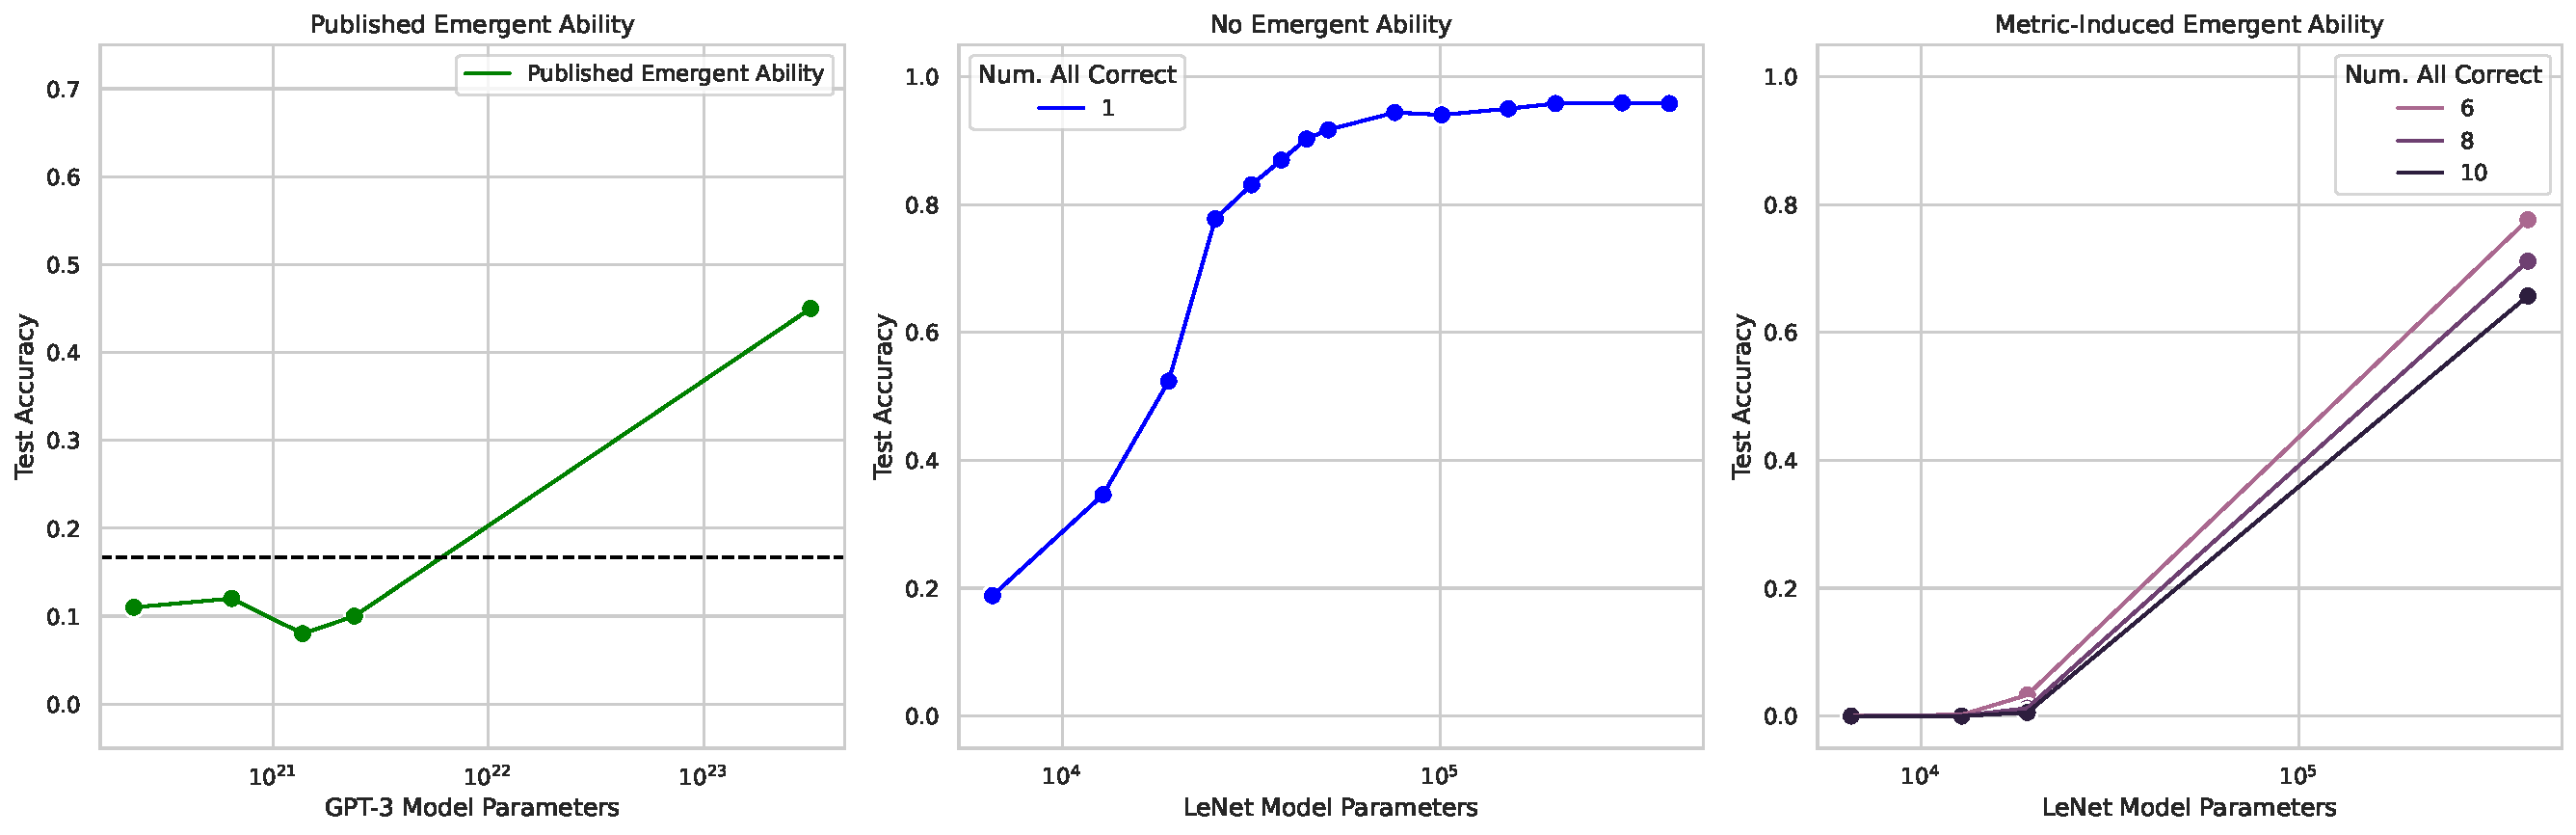
\includegraphics[width=\textwidth]{figures/vision/no_emergence_and_emergence_dataset=mnist.pdf}
    \caption{\textbf{Induced emergent MNIST classification ability in convolutional networks.} (A) A published emergent ability from the BIG-Bench Grounded Mappings task \cite{wei2022emergent}. (B) LeNet trained on MNIST \cite{lecun1998mnist} displays a predictable, commonplace sigmoidal increase in test accuracy as model parameters increase. (C) When accuracy is redefined as correctly classifying $K$ out of $K$ independent test data, this newly defined metric induces a seemingly unpredictable change.}
    \label{fig:vision_mnist}
\end{figure}

We begin by inducing an emergent classification ability in a LeNet convolutional neural network family \cite{lecun1998gradient}, trained on the MNIST handwritten digits dataset \cite{lecun1998mnist}.
This family displays smoothly increasing test accuracy as the number of parameters increase (Fig. \ref{fig:vision_mnist}B).
To emulate the accuracy metric used by emergence papers \cite{ganguli2022predictability, wei2022emergent, srivastava2022beyond}, we use \textit{subset accuracy}: 1 if the network classifies $K$ out of $K$ (independent) test data correctly, 0 otherwise.
Under this definition of accuracy, the model family displays an ``emergent" ability to correctly classify sets of MNIST digits as $K$ increases from $1$ to $5$, especially when combined with sparse sampling of model sizes (Fig. \ref{fig:vision_mnist}C).
This convolutional family's emergent classification ability qualitatively matches published emergent abilities, e.g., at the BIG-Bench Grounded Mappings task \cite{wei2022emergent} (Fig. \ref{fig:vision_mnist}A).



\end{document}
